\chapter{Search for top-quark pair associated Higgs production}
\label{sec:tth}
In this chapter, we describe the search for~\ttHbb\xspace using the matrix element method at the CMS experiment (MEM) in Run 2 of the LHC. This is based on preliminary results from CMS~\cite{CMS:2016qwm,CMS:2016zbb} and ongoing work. We concentrate on the semileptonic (SL) and dileptonic (DL) decay channels of the top quark pair and the application of the MEM in this search, where the primary background arises from QCD production of \ttbar+jets. We are showing results with the 2016 dataset of CMS data, the use of which for this thesis has been endorsed by the CMS Higgs group.

\begin{figure}
\begin{centering}
\subfloat{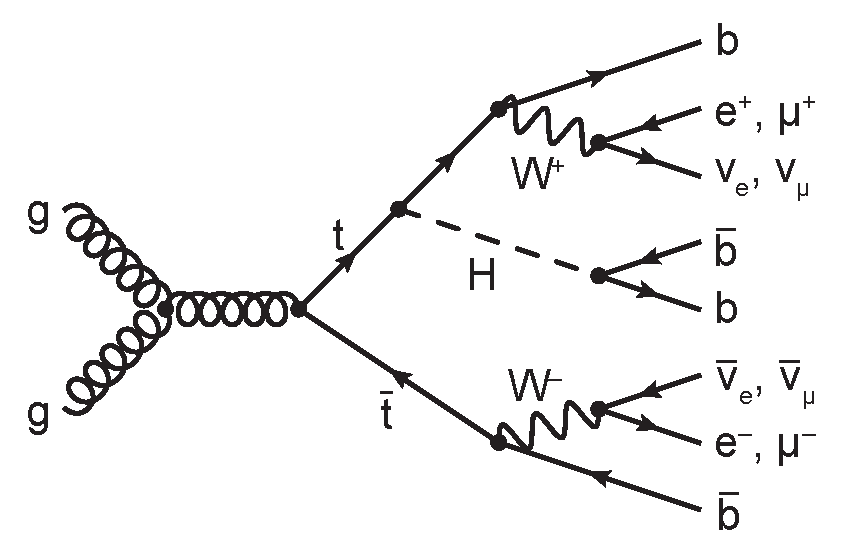
\includegraphics[width=0.3\textwidth]{figures/tth/tth_dl_feyn.pdf}}
\subfloat{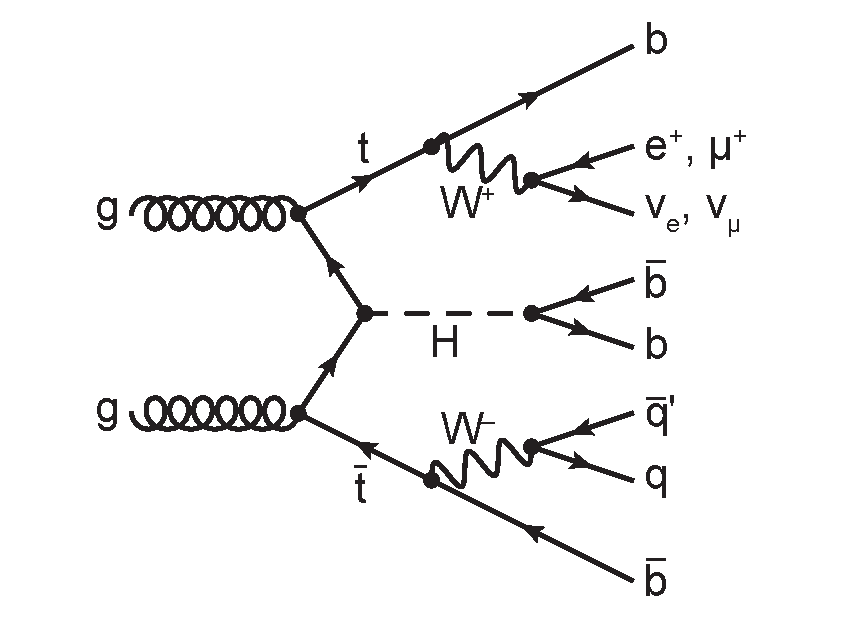
\includegraphics[width=0.3\textwidth]{figures/tth/tth_sl_feyn.pdf}} \\
\caption[Representative leading-order Feynman diagrams for the \ttHbb\xspace process]{Representative leading-order Feynman diagrams for the \ttHbb\xspace process in the gluon-fusion production channel. On the left, we show the dileptonic (DL) decay of the top quark pair, whereas on the left, we show the semileptonic (SL) decay channel.}
\label{fig:tth_diagrams}
\end{centering}
\end{figure}

Briefly, the analysis proceeds as follows. Throughout the analysis, we use the MC simulation and data samples described in~\cref{sec:data_mc}. The detailed identification criteria for the physics objects (jets and leptons) are motivated by established top quark analyses and are described in~\cref{sec:object_id}. The selection is motivated by the semileptonic and dileptonic decays of the top quark pair, which results in a final state containing several jets, charged leptons and \MET. We select events with at least one (two) charged lepton(s) in the semileptonic (dileptonic) channel and at least four jets, out of which three must be b~tagged.

The statistical analysis is described in~\cref{sec:analysis}. We further divide the events into independent categories based on the jet and b~tag multiplicity, as described in~\cref{sec:event_selection}. These categories are introduced in order to constrain the various sub-processes of~\ttbar+jets, described further in~\cref{sec:ttbar_subprocesses}, together with the \ttH~signal cross-section. In order to extract the signal strength modifier~$\mu = \sigma/\sigma_{\mathrm{SM}}$ for the \ttH~process, we perform a combined template fit in all the categories, relying on the discriminating power provided by the MEM in categories with a high signal-to-background ratio and on other multivariate techniques in background-enhanced control regions. The fit is described in~\cref{sec:statistical_method}.

An important component in the fit is the handling of systematic uncertainties, which drives the determination of the confidence interval of the estimated signal strength and is described in~\cref{sec:systematic_unc}. We study the fit model with respect to the systematic uncertainties in~\cref{sec:model_analysis} before determining the compatibility of the model with data. Finally, we present the results of the analysis in~\cref{sec:tth_results}, followed by a discussion in ~\cref{sec:tth_discussion} and a summary and outlook in~\cref{sec:tth_summary}.

\section{Data and simulation}
\label{sec:data_mc}

We use proton-proton collision data collected by the CMS experiment at a center-of-mass energy of~$\sqrt{s} = 13~\mathrm{TeV}$, corresponding to a total integrated luminosity of~$35.9~\ifb$~in the semileptonic (SL) and dileptonic (DL) channels. We have used the complete dataset of 2016 as an update over the analysis finalised in the middle of 2016, which used roughly $12.9~\ifb$ of data~\cite{CMS:2016zbb}.

We use MC simulation to model the signal and background processes, interfaced to a parton shower and hadronisation as appropriate. In order to model the detector effects, we use a detailed simulation of the detector based on \geant~\cite{Agostinelli:2002hh}. For the~\ttH~signal, \ttbar+jets and single-top backgrounds, we use the NLO generator \powheg~\cite{Frixione:2007vw,Re:2010bp}. The use of an NLO model for the signal and the primary background processes is a significant advancement over Run I \ttH~analyses at the LHC, where only a LO model was available. Besides~\ttbar+jets, we need to model the production of W or Z/$\gamma^*$~bosons with additional jets (denoted W/Z+jets or commonly V+jets), which is simulated using \madgraphatnlo (v. 2.2.2)~\cite{Hirschi:2011pa} and diboson production (WW, WZ, ZZ), simulated using \pythia~\cite{Sjostrand:2007gs}. Throughout, we assume the value of the top quark mass to be~$m_t \simeq 172.5\GeV/c^2$~and of the Higgs boson to be~$m_H \simeq 125\GeV/c^2$. In order to describe the substructure of the protons via the parton density functions, we use the PDF parametrisation provided by NNPDF3.0 and~\pythia~for showering and hadronisation.

In order to model the production of hadrons, the parameters in the~\pythia~model have been tuned to Tevatron, LEP and LHC data~\cite{CMS-PAS-GEN-14-001,Skands:2014pea}. It has been observed that the default tune in~\pythia~does not reproduce the observed number of jets in data in the~\ttbar+jets dominated region~\cite{CMS:2016kle}. Therefore, CMS has created a custom tune where the~$\alpha_{\mathrm{ISR}}$ parameter, which controls the amount of initial-state radiation, and~$h_{\mathrm{damp}}$ parameter, which suppresses real emissions in~\powheg, have been adapted to reproduce the spectrum of the number of jets observed at CMS~\cite{CMS-PAS-TOP-16-021}. This MC tuning has been carried out on~$\sqrt{s} = 8~\TeV$~data and significantly improves the modelling of the jet multiplicity.

\begin{table}[h!]
\begin{center}
\begin{tabular}{cccc}
\hline
sample & generator & events & cross-section \\
\hline
\ttHbb\xspace & \powheg & 3~845~992 & 0.293~pb~\cite{deFlorian:2016spz} \\
\ttHnonbb & \powheg & 3~981~250 & 0.215~pb~\cite{deFlorian:2016spz} \\
\hline
\ttbar+jets (SL) & \powheg & 152~720~952 & 365.45~pb~\cite{Czakon:2011xx} \\
\ttbar+jets (DL) & \powheg & 79~092~400 & 88.34~pb~\cite{Czakon:2011xx} \\
\hline
\ttbar+W($\rightarrow \mathrm{\ell \nu}$) & \madgraphatnlo & 5~280~565 & 0.2043~pb~\cite{Alwall:2014hca} \\
\ttbar+W($\rightarrow \mathrm{qq'}$) & \madgraphatnlo & 833~298 & 0.4062~pb~\cite{Alwall:2014hca} \\
\ttbar+Z($\rightarrow \mathrm{\ell\ell, \nu\nu}$) & \madgraphatnlo & 13~908~701 & 0.2529~pb~\cite{Alwall:2014hca} \\
\ttbar+Z($\rightarrow \mathrm{qq'}$) & \madgraphatnlo & 749~400 & 0.5297~pb~\cite{Alwall:2014hca} \\
\hline
WW & \pythia & 7~981~136 & 118.7~pb~\cite{Gehrmann:2014fva} \\
WZ & \pythia & 1~988~098 & 47.13~pb~\cite{Campbell:2011bn} \\
ZZ & \pythia & 3~995~828 & 16.523~pb~\cite{Campbell:2011bn} \\
\hline
single top (tW) & \powheg, 4FS & 992~024 & 35.85~pb~\cite{Kidonakis:2010ux} \\
single (anti)top (tW) & \powheg, 4FS & 998~276 & 35.85~pb~\cite{Kant:2014oha} \\
single top (t) & \powheg, 5FS & 5~993~676 & 136.02~pb~\cite{Kant:2014oha} \\
single (anti)top (t) & \powheg, 5FS & 3~928~063 & 80.95~pb~\cite{Kant:2014oha} \\
single top (s), $(\mathrm{W\rightarrow \ell\nu})$ & \madgraphatnlo, 4FS & 3~928~063 & 3.70~pb~\cite{Kant:2014oha} \\
\hline
W+jets $(\mathrm{W\rightarrow \ell\nu})$ & \madgraphatnlo & 29~705~748 & 61526.7~pb~\cite{Gavin:2012sy} \\
$\mathrm{Z \rightarrow \ell \ell+jets}, m_{\ell\ell} < 50$~GeV & \madgraphatnlo & 35~291~566 & 18610~pb~\cite{Melnikov:2006kv} \\
$\mathrm{Z \rightarrow \ell \ell+jets}, m_{\ell\ell} \geq 50$~GeV & \madgraphatnlo & 145~803~217 & 5765.4~pb~\cite{Melnikov:2006kv} \\
\hline
\hline
\end{tabular}
\caption[The MC samples used in the~\ttHbb\xspace analysis]{The MC samples used in the~\ttHbb\xspace analysis. For the simulation of the parton shower and subsequent hadronisation, \pythia\xspace is used for all samples, whereas \powheg\xspace or \madgraphatnlo\xspace are used for the hard process. The single top tW-channel process is simulated in the four flavour scheme (4FS), whereas other processes use the five flavour scheme (5FS) with a massless b~quark being present in the proton.}
\label{tab:mc_samples}
\end{center}
\end{table}

\begin{table}[h!]
\begin{center}
\begin{tabular}{c|cccc}
\hline
dataset & trigger threshold & data taking period & integrated luminosity \\
\hline
single muon & 24 GeV & Run B-H, 2016 &~$35.9~\ifb$~\\
single electron & 27 GeV & Run B-H, 2016 &~$35.9~\ifb$~\\
dimuon & 17 (8) GeV & Run B-H, 2016 &~$35.9~\ifb$~\\
dielectron & 23 (12) GeV & Run B-H, 2016 &~$35.9~\ifb$~\\
muon, electron & $23_\mu~(12_e)$, $23_e~(8_\mu)$ GeV & Run B-H, 2016 &~$35.9~\ifb$~\\
\hline
\hline
\end{tabular}
\caption[The data samples used in the~\ttHbb\xspace  analysis]{The data samples used in this analysis. We list the transverse momentum thresholds in the trigger for the leading (subleading) charged leptons.}
\label{tab:data_samples}
\end{center}
\end{table}

We list the details of the MC samples in~\cref{tab:mc_samples} and of data in~\cref{tab:data_samples}. In order to compare simulation to data, the simulated events are weighted according to the integrated luminosity and the predicted cross sections, which are taken from the best available inclusive calculations. In particular, the~\ttH~cross section is known at NLO accuracy~\cite{Dittmaier:1318996,Beenakker:2001rj,Beenakker:2002nc,Dawson:2002tg,Dawson:2003zu}. The Higgs boson branching fraction for~\Hbb~is affected by radiative corrections that are known up to N4LO (QCD) and NLO (electroweak), resulting in an uncertainty of about 1-2\%~\cite{Djouadi:1997yw,Butterworth:2010ym,deFlorian:2016spz}.
The inclusive cross section for~\ttbar production is known at NNLO accuracy and includes soft gluon resummation to next-to-next leading log (NNLL)~\cite{Czakon:2011xx}. The cross-sections of the minor backgrounds are known to at least NLO, as summarised in~\cref{tab:mc_samples}.

In addition to the hard interaction and the subsequent showering and hadronisation, events from additional pp interactions within the same bunch crossing (pileup) are superimposed on the simulated event for all processes. The multiplicity distribution of these additional pileup events is reweighted to match the observed number of interactions in data. Furthermore, we correct the MC simulation with additional data-driven correction factors for b~tagging and lepton efficiencies as described in~\cref{sec:systematic_unc}.

%\fixme: PU plot

\subsection{Modelling of \ttbar+jets}
\label{sec:ttbar_subprocesses}
The main background in the \ttHbb~search is the QCD production of~\ttbar+jets, for which we are using an NLO model based on \powheg. This process is affected by considerable scale uncertainties at the level of 70-80\% at LO and reduced to about 20-30\% at NLO~\cite{deFlorian:2016spz}. Furthermore, there are multiple scales present in the \ttbb~process, with a large hierarchy between the scale set by the top quark mass and the mass of the bottom quark pair. Despite the available NLO QCD corrections, at high jet multiplicities, the differential distributions are modelled only at LO or parton shower accuracy, depending on the momenta and multiplicity of jets. Therefore, the residual uncertainties in~\ttbar+heavy flavour production are significant in terms of the differential distributions, with the differences of up to 100\% between the \powheg\ and \madgraphatnlo\ MC models in variables sensitive to parton shower and quark mass effects~\cite{deFlorian:2016spz}. In general, to have an effective treatment of high-multiplicity events in a precise~\ttHbb\xspace measurement, an improved theoretical understanding of the underlying QCD process for $\mathrm{pp} \rightarrow \mathrm{t\bar{t}b\bar{b}}$, along with possible interference effects with the signal process is necessary~\cite{Denner:2014wka}.

In the absence of an experimentally verified model that accurately describes these high-multiplicity and heavy flavour processes, we account for these modelling uncertainties by assigning conservative uncertainties on the theoretical modelling. We subdivide the~\ttbar+jets sample based on the generator-level flavour of additional jets, as the underlying processes that give rise to these different flavour categories are different. In particular, it has been shown that \ttbb~can be significantly affected by the modelling of gluon splitting to collinear bottom quarks~\cite{Cascioli:2013era}. We distinguish between the following \ttbar+jets sub-processes:
\begin{itemize}
\item \ttbb, where two additional bottom jets are created from one or more b hadrons,
\item \ttb, with only one additional bottom jet, which can arise from a process with two b hadrons, with one b hadron being out of acceptance,
\item \tttwob, where jets from two b hadrons merge to produce one resolved bottom jet, which can arise from collinear gluon splitting,
\item \ttcc, if there are no additional bottom jets but at least one charm flavoured jet,
\item \ttlf (light flavour), in case there are no bottom or charm flavoured jets.
\end{itemize}
The jet flavour is assigned using so-called \textit{ghost clustering}, where simple geometrical matching between partons and jets is superseded by clustering the generator-level partons and hadrons along with the detector-level jet constituents using standard jet algorithms. Information from the generator-level decay chain is used to assign the flavour of the jet according to the parton that gave rise to that jet~\cite{Bartosik:2047049}, such that only hadrons that did not arise from the decay chain of a top quark are used in this categorisation. The aim of this splitting is to have experimental constraints on the uncertainties of the various~\ttbar~sub-processes separately, effectively relaxing some of the modelling assumptions. We illustrate the differences in the modelling of these processes in~\cref{fig:tth_ttjets_subprocesses} by comparing the distributions of leading jet transverse momentum ($p_T$) and the mass of the geometrically closest b jet pair $m_{\mathrm{b\bar{b}}}$, with significant differences between distributions visible for these processes.

\begin{figure}
\begin{centering}
\subfloat[Leading jet $p_T$]{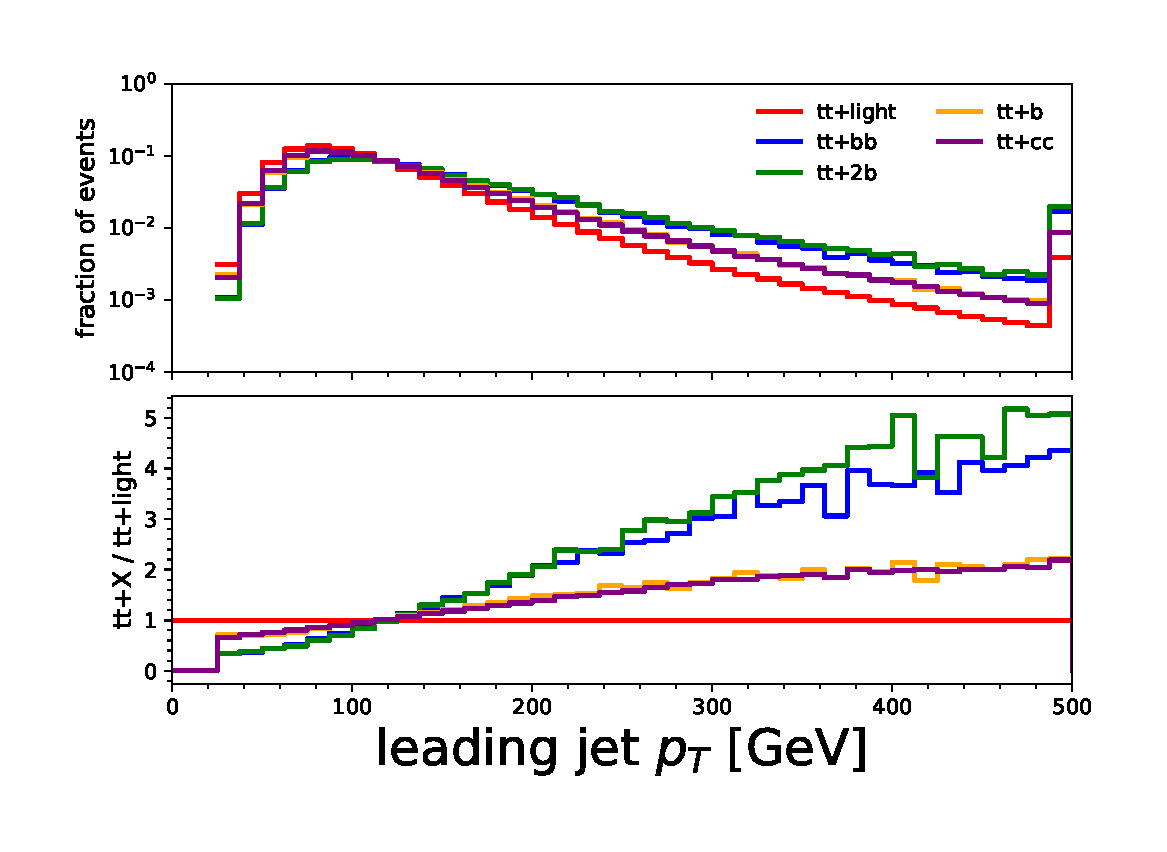
\includegraphics[width=0.5\textwidth]{figures/tth/ttx_jet_pt.pdf}}
\subfloat[The invariant mass of the closest b jet pair]{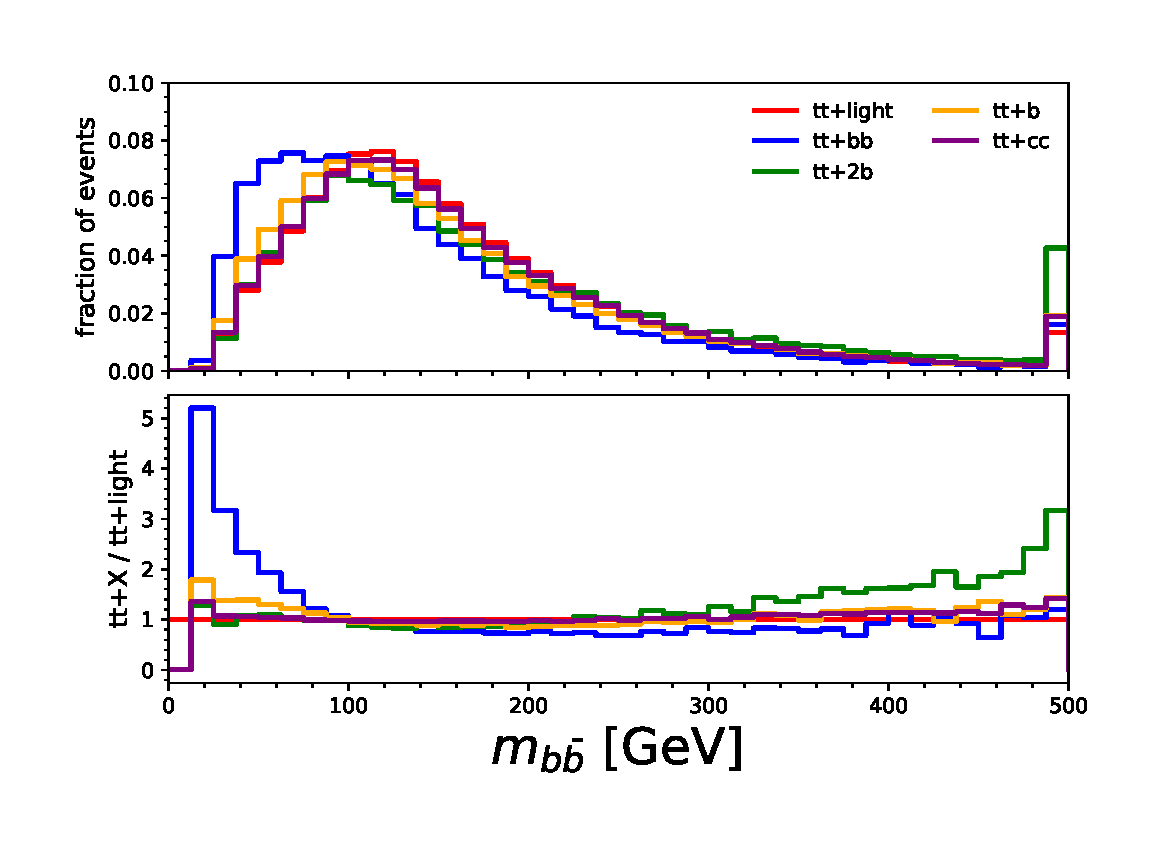
\includegraphics[width=0.5\textwidth]{figures/tth/ttx_mbb.pdf}} \\
\caption[Modelling of the \ttbar+X sub-processes]{The modelling of the leading jet transverse momentum (\textbf{a}) and the invariant mass of the closest b jet pair (\textbf{b}) for the various \ttbar+jets sub-processes based on the \ttbar+jets POWHEG simulation from events with at least two jets with $p_T > 30$~GeV, $|\eta| < 2.5$.}
\label{fig:tth_ttjets_subprocesses}
\end{centering}
\end{figure}

\section{Event reconstruction and object identification}
\label{sec:object_id}
We use particle flow to reconstruct events from particle candidates based on signals from all sub-detectors, as described in~\cref{sec:particleflow}. This allows us to perform the analysis at the level of physics objects, namely, jets, charged leptons and \MET~from neutrinos, which arise from the decay of the top quark pair. A top quark decays almost exclusively through $\mathrm{t} \rightarrow \mathrm{W}^+ \mathrm{b}$, such that the leptonic or hadronic decay of the W-boson, which happen with a branching ratio of 33\% or 67\% respectively, determines the final state. In the case of the semileptonic decay, which happens with a total branching ratio of 44\%, we expect one charged lepton ($\mathrm{e}^\pm, \mathrm{\mu}^\pm$), \MET~from the corresponding neutrino, at least six jets, out of which four arise from bottom quarks and two from light quarks from the W-boson decay. In the dileptonic decay of the top quark pair, which happens with a branching ratio of $\simeq11\%$, we expect two charged leptons of opposite sign, \MET~from neutrinos and at least four jets, all of which arise from bottom quarks. The fully hadronic decay of the top quark pair is treated in a separate analysis at CMS, as the background processes and required triggers are significantly different between the leptonic and hadronic channels. The hadronic analysis~\cite{CMS:2017_tthfh} makes use of a discriminator based on matrix elements between the \ttH~signal and the multi-jet background that is similar to the method developed for the leptonic channel. The possible final state configurations are shown in~\cref{fig:tth_finalstate}.


\begin{figure}
\begin{centering}
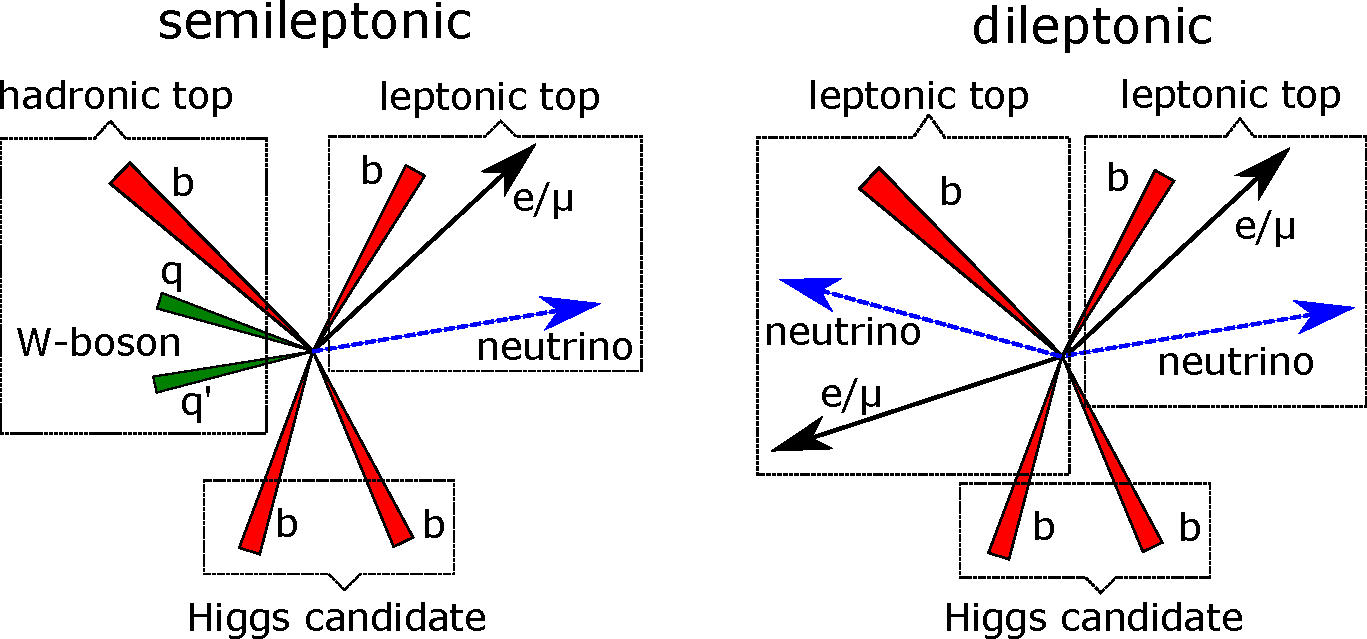
\includegraphics[width=0.8\textwidth]{figures/tth/finalstate.pdf}
\caption[\ttHbb~leptonic final states]{The semileptonic (left) and dileptonic (right) final states of \ttHbb.}
\label{fig:tth_finalstate}
\end{centering}
\end{figure}


\subsection{Charged leptons}
\label{sec:object_id_lep}

The leptonic decay of at least one of the W-bosons from top decay is required in order to trigger the event at the HLT. In order to suppress leptons from the multi-jet QCD background, the charged leptons are required to be sufficiently isolated from hadronic activity using an isolation variable, which is computed within a cone of radius~$\Delta R$~around the lepton direction (defined by the track) from the primary vertex as shown in~\cref{eq:iso_mu} for muons and~\cref{eq:iso_el} for electrons. In order to compute the isolation, we sum over the transverse momenta of all particle candidates ($p_T^{c.h.}$~for charged hadrons,~$E_T^{n.h.}$~for neutral hadrons,~$E_T^{\gamma}$~for photons) excluding the lepton itself and subtracting the neutral component from pileup events based on either the average pile-up energy ($\rho$) and effective area ($A$) for electrons or pile-up associated charged hadrons for muons~\cite{Cacciari:2007fd}. The pre-factor~$1/2$~for the pile-up component for muons is used to account for the approximate charged-to-neutral fraction in the hadronisation of pile-up interactions~\cite{CMS:2012}.

Furthermore, in order to suppress leptons from non-prompt decays, we apply identification (ID) criteria based on various reconstruction parameters for the leptons. For muons, we apply the \textit{tight ID}, which is a cut-based selection that suppresses decays in flight and is based on properties of the global track fit, number of hits in the pixel detector, tracker and muon chambers and sufficient proximity to the primary vertex~\cite{Chatrchyan:2012xi,CMS:2017_muon_pog}. For electrons, the ID is based on a multivariate discriminator combining track-to-cluster matching observables, super cluster structure and cluster shapes~\cite{Khachatryan:2015hwa,CMS:2017_egamma_pog}.

We summarise the lepton selection criteria in all the considered channels in~\cref{tab:lepton_selection} and describe the event selection in terms of leptons further in~\cref{sec:event_selection}.

\begin{equation}
\label{eq:iso_mu}
\mathrm{Iso}_{\mathrm{\mu}} = \sum_{\Delta R < 0.4} p_T^{c.h.} + \mathrm{max}\biggl(0, \sum_{\Delta R < 0.4} [E_T^{n.h.} + E_T^{\gamma} - \frac{1}{2} p_T^{\mathrm{PU}}] \biggr)
\end{equation}

\begin{equation}
\label{eq:iso_el}
\mathrm{Iso}_{\mathrm{e}} = \sum_{\Delta R < 0.3} p_T^{c.h.} + \mathrm{max}\biggl(0, \sum_{\Delta R < 0.3} [E_T^{n.h.} + E_T^{\gamma} - \rho A(\eta)] \biggr)
\end{equation}

\begin{table}[h!]
\begin{center}
\label{tab:lepton_selection}
\begin{tabular}{c|ccccc}
\hline
channel & trigger & offline~$p_T$~&~$|\eta|$~& isolation \\
\hline
$\mathrm{\mu}^\pm$~&~$p_T > 24\GeV$~&~$p_T > 25\GeV$~&~$|\eta| < 2.1$~& ~$\mathrm{Iso}/p_T < 0.15$~\\

$\mathrm{e}^\pm$~&~$p_T > 27\GeV$~&~$p_T > 30\GeV$~&~$|\eta| < 2.1$~&~$\mathrm{Iso}/p_T < 0.15$\\

$\mathrm{e}^\pm\mathrm{e}^\mp$~&~$p_T > 23 (12)\GeV$~&~$p_T > 25 (15)\GeV$~&~$|\eta| < 2.1$~&~$\mathrm{Iso}/p_T < 0.15$\\

$\mathrm{e}^\pm\mathrm{\mu}^\mp$~&~$p_{T} > 23_{\mathrm{e}} (8_{\mathrm{\mu}})\GeV$~&~$p_T > 25 (15)\GeV$~&~$|\eta| < 2.4$~&~$\mathrm{Iso}/p_T < 0.25_{\mathrm{\mu}} (0.15_{\mathrm{e}})$~\\

$\mathrm{\mu}^\pm\mathrm{e}^\mp$~&~$p_{T,} > 23_{\mathrm{\mu}} (12_{\mathrm{e}})\GeV$~&~$p_T > 25 (15)\GeV$~&~$|\eta| < 2.4$~&~$\mathrm{Iso}/p_T < 0.25_{\mathrm{\mu}} (0.15_{\mathrm{e}})$~\\

$\mathrm{\mu}^\pm\mathrm{\mu}^\mp$~&~$p_T > 17 (8)\GeV$~&~$p_T > 25 (15)\GeV$~&~$|\eta| < 2.4$~&~$\mathrm{Iso}/p_T < 0.25$~\\

\hline
\hline
\end{tabular}
\caption{The selection and ID criteria for the charged leptons.}
\end{center}
\end{table}

\subsection{Jets}
\label{sec:object_id_jets}
As the signal process is expected to produce between four to six jets in the leading order description and additional jets due to QCD radiation and pileup, an accurate reconstruction of jets is critical for this analysis. We use the anti-$k_T$~clustering algorithm~\cite{Cacciari:2008gp} in the \texttt{FASTJET} implementation~\cite{Cacciari:2011ma} with a distance parameter $\Delta R=0.4$ to reconstruct jets from particle flow candidates~\cite{CMS:2010xta,CMS:2009nxa,CMS:2010byl} and use the CMS particle flow (PF) jet ID algorithm, described in~\cref{sec:particleflow}, to reject reconstruction failures and noise. The noise rejection works on the basis of cuts on jet energy fractions from various types of PF candidates, namely muons, electrons, photons, charged hadron and neutral hadron candidates and has a noise rejection of around 99\%~\cite{CMS:2017wyc}.

\subsubsection{Charged hadron subtraction}
Charged particles from pileup interactions are removed from clustering via the process of charged hadron subtraction (CHS). As CHS relies on the reconstruction of tracks and the association of charged hadrons to tracks, the procedure is applied within the tracker volume ($|\eta| < 2.5$). We choose the leading primary vertex (PV) as the one that has the highest magnitude of total track transverse momentum squared ($\sum |p_T^{\mathrm{track}}|^2$), with the rest of the PVs passing certain quality criteria as subleading PVs. Charged hadrons that are associated to tracks that are compatible with subleading PVs are removed. The subtraction procedure reduces the amount of jets arising from pileup from about 20\% to 5\% in the tracker region and also improves the momentum resolution and angular resolution ($\Delta R \simeq 0.01$) of jets~\cite{CMS:2014ata}.

\subsubsection{Jet energy scale calibration}
\label{sec:jes_calibration}
The experimentally measured energies of the jets have to be calibrated in terms of jet energy scale (JES) and resolution (JER) in both data and simulation. This is done using jet energy corrections (JEC), which correct for offset energy from pileup, the detector response based on simulation, the residual differences between data and simulation based on well-understood channels such as di-jet production, and the detector response to jet flavour. 

The presence of pileup interactions generates a diffuse energy component that results in an energy offset in the jets. This offset correction is estimated using simulation by comparing jets in a MC sample without pileup events to the same simulation overlayed with pileup, geometrically matching them to the same underlying jet on the generator level~\cite{cms_jec_2017}. An additional scale factor between data and simulation is extracted from zero-bias data using the random cone method~\cite{Chatrchyan:2011ds}.  

The detector response is defined as the ratio between the reconstructed jet and a geometrically matched particle-level jet, averaged over a sample of jets:~$R = \langle p_T \rangle / \langle p_{T,\mathrm{particle}} \rangle$. It is estimated using a detailed model of the detector geometry, alignment and calibration, implemented in \texttt{GEANT4} and evaluated in bins of particle-level jet momentum and reconstructed jet~$\eta$. The corrections bring the response to a deviation of approximately 1\% from unity based on simulations. A residual data to simulation correction scale factor is applied on data based on transverse momentum balance from dijet,~$\mathrm{Z}/\gamma^*$+jets and multi-jet events, with the momentum projection fraction (MPF) with respect to the missing transverse momentum being used as an alternative derivation for the corrections. These relative corrections rely on comparing the jet under calibration (probe) to a reference object (tag) and are of the order of a few percent in the central region considered in this analysis~\cite{Chatrchyan:2011ds,cms_jec_2017}.

The jet flavour response is estimated using simulation by taking the difference between the jet response for quark and gluon jets as predicted by ~\pythia~and~\herwig. The magnitude of the flavour response is generally within a few percent, with differences between the flavours arising from fragmentation, where gluons fragment the most into soft particles that may remain unreconstructed and thus have the lowest response, and particle composition, with the neutral hadronic component having the largest effect. The flavour corrections are validated in Z+b~jet data and the residual correction between data and simulation is found to be consistent with unity~\cite{Chatrchyan:2011ds}.

\subsubsection{Jet energy resolution}
In contrast to jet energy scale, which is known with a total uncertainty better than~$3\%$~over the relevant phase space, the jet energy resolution is known to around~$10-20\%$. The resolution can be determined using~$p_T$~balance as for JES, but measuring the width instead of the mean of the response distribution. Both~$\mathrm{Z}/\gamma^*$+jet and dijet events are used to determine the JER response~\cite{Chatrchyan:2011ds}. In the implementation of the MEM, we also use approximate jet resolution functions derived from simulation in order to account for detector effects in the phase space integral as explained in~\cref{sec:transfer_functions}.

\subsection{B~tagging}
\label{sec:object_id_btag}

Since the \ttHbb\xspace signal is characterised by the presence of four bottom quarks in the final state, with two arising from the top quarks and two from the Higgs boson decay, an accurate identification of b~jets arising is important in this analysis. We rely on the combined secondary vertex algorithm (CSVv2)~\cite{Chatrchyan:2012jua} to identify b jets. The CSVv2 algorithm uses secondary vertex properties such as the impact parameter along with track-based lifetime information to create a robust combined discriminator~$\xi$~optimised to distinguish between jets arising from bottom quarks and light quarks using supervised learning. In Run 2 of the LHC, the CSVv2 algorithm has been improved with a new vertex reconstruction algorithm, as well as using artificial neural networks instead of a likelihood method to combine the input variables, such that correlations between the inputs are taken into account, as described in~\cref{sec:btagging}.

The threshold value of the b~tagging discriminant, above which a jet is considered to be b~tagged is chosen such that the efficiency of misidentifying jets arising from light quarks (u,d,s) or gluons as b~jets would be around $\simeq1\%$. This corresponds to an efficiency of $\simeq70\%$~of correctly identifying bottom quarks and of around~$\simeq20\%$ for mis-identifying charm quarks. This threshold value is denoted the CSVv2 medium working point (CSVM) and an event where $N$ jets pass this threshold contains $N$ b~tags.

\subsubsection{B~tagging likelihood}
We further use the values of the per-jet b~tagging discriminants~$\vec{\xi} = [\xi_1, \xi_2, \dots, \xi_{N_j}]$ with $N_j$ being the number of jets to construct a per-event likelihood discriminator $\mathcal{BLR}(\vec{\xi})$ between the hypotheses that the event contained four bottom quarks (``$4\mathrm{b}$'') or two bottom quarks (``$2\mathrm{b}$'').

First, we use the probability density that the~$k$-th jet has a discriminator value~$\xi_k$~assuming that it originated from a bottom quark (light quark), $f(\xi_k | \mathrm{b})$~[$f(\xi_k | \mathrm{l})$], to define a likelihood for the given observed discriminator values $\vec{\xi}$ to result from $M$ bottom quarks~$\mathcal{BL}(\vec{\xi} | M\mathrm{b})$, as shown in~\cref{eq:blr}.

\begin{equation}
\label{eq:blr}
\mathcal{BL}(\vec{\xi} | M\mathrm{b}) = \sum_{i \in C_{M,N}} \biggl[ \prod_{k \in \mathrm{b}_i} f(\xi_k | \mathrm{b}) \prod_{k \in \mathrm{l}_i} f(\xi_k | \mathrm{l}) \biggr]
\end{equation}

The sum in~\cref{eq:blr} is performed over all the combinations $C_{M,N}$ of associating~$M$~jets out of~$N$~to bottom quarks and the rest to light quarks, such that~$\mathrm{b}_i$~($\mathrm{l}_i$) refers to the~$M$~($N-M$) jets associated to bottom quarks (light quarks) in the~$i$-th combination. There are $\frac{N!}{(N-M)!M!}$ unique combinations to choose $M$ jets to be b~tagged out of $N$ jets. For example, for $M=4$ and $N=6$, the combinations $C_{M,N}$ are formed by dividing up the jet indices $k=1\dots6$ between the b~quark and light quark hypotheses, with one combination out of 15 being $b_i = \{1,2,3,4\}$, $l_i = \{5,6\}$.

The likelihoods for hypotheses with a particular number of bottom quarks are then used to construct a likelihood ratio discriminator~$\mathcal{BLR}(\vec{\xi})$~(\cref{eq:blr_ratio}) that is optimised to suppress the~\ttlf~background with two bottom quarks in favour of the~\ttHbb\xspace signal with four bottom quarks.

\begin{equation}
\label{eq:blr_ratio}
\mathcal{BLR}(\vec{\xi}) = \frac{\mathcal{BL}(\vec{\xi} | 4\mathrm{b})}{\mathcal{BL}(\vec{\xi} | 4\mathrm{b}) + \mathcal{BL}(\vec{\xi} | 2\mathrm{b})}
\end{equation}

We assess the performance of this discriminator in terms of \ttHbb\ vs.~\ttlf~discrimination using simulation. In~\cref{fig:blr_discrimination}, we see that the~$\mathcal{BLR}$~discriminant improves over a fixed cut of~$\ge4$~jets passing the CSVv2 medium working point ($N_{\mathrm{CSVM}} \ge 4$) by about 50\% ($\epsilon_{\ttlf} = 0.04\% \rightarrow 0.022\%$) in terms of background rejection at the same signal efficiency ($\epsilon_{\ttHbb} \simeq 7\%$).

Furthermore, we have studied the efficiency of the $\mathcal{BLR}$~in correctly reducing the number of permutations in the MEM by assigning jets to be b~tagged or untagged. For this, we evaluated the fraction of events where the final jets can be correctly matched to quarks from the hard interaction as a function of~$\mathcal{BLR}$. We see in~\cref{fig:blr_matching} that the likelihood discriminator is positively correlated with the probability that all the quarks have been matched to jets, where around~$50\%$~of bottom quarks from top decay, $40\%$~of bottom quarks from Higgs decay and around~$20\%$~of the light quarks from the W boson decay have been reconstructed as jets at~$\mathcal{BLR} \simeq 0.8$. Furthermore, we see a positive correlation between the likelihood discriminator and the probability that the highest-probability permutation in the sum in~\cref{eq:blr} with the~$4$~bottom quark hypothesis corresponds to the bottom quarks from top or Higgs decay. In other words, the likelihood discriminator successfully tags the bottom quarks on an event-by-event basis.

\begin{figure}
\begin{centering}
\subfloat[Simulated shape of the discriminant.]{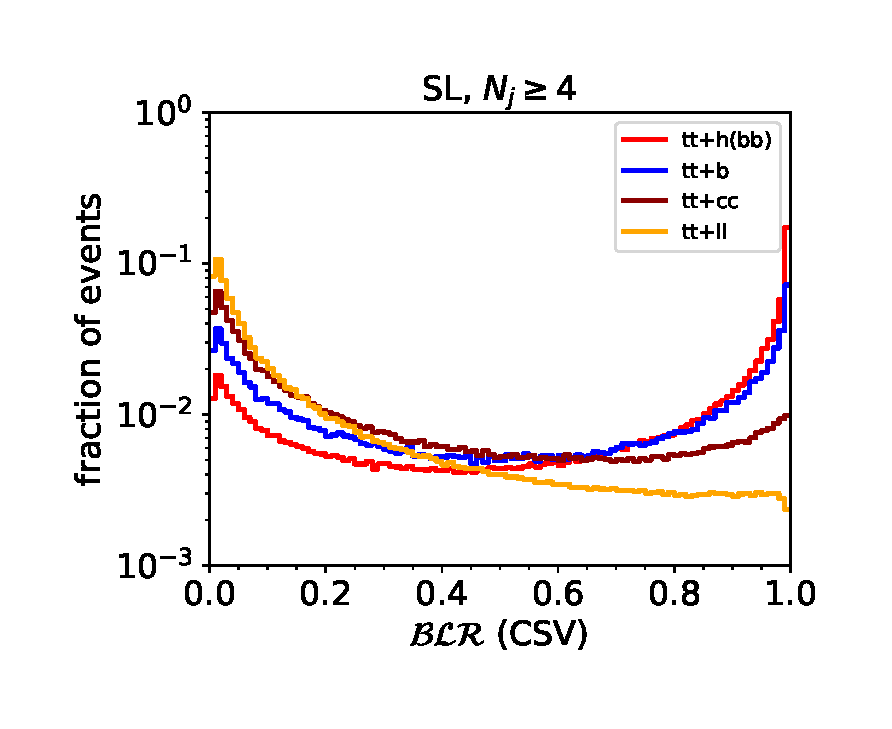
\includegraphics[width=0.5\textwidth]{figures/blr_shape_btagCSV.pdf}} 
\subfloat[Expected performance of the discriminant.]{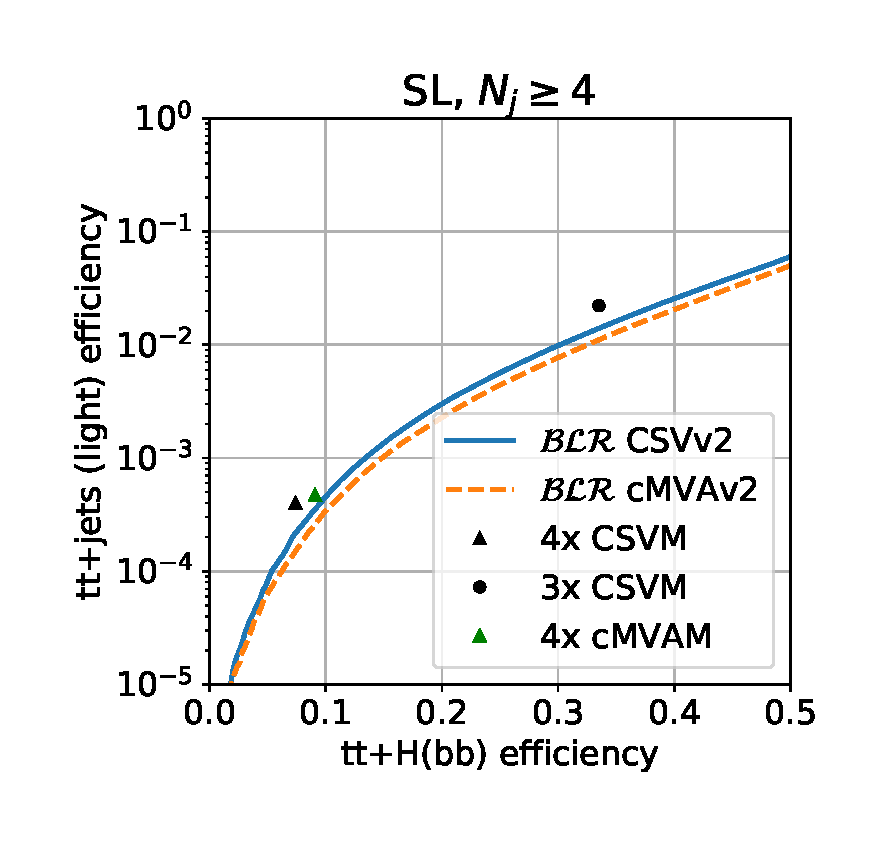
\includegraphics[width=0.5\textwidth]{figures/blr_roc.pdf}}\\
\caption[Expected performance of the b~tag likelihood ratio discriminant.]{Simulated distribution and expected performance of~$\mathcal{BLR}$~discriminant in the SL channel, requiring at least four good jets. On~(\textbf{a}), we show the simulated shapes of the discriminant for signal~(\ttHbb) and the various \ttbar+jets backgrounds. On~(\textbf{b}), we compare the efficiency to select~\ttHbb\xspace and~\ttlf~events. We see that the~$\mathcal{BLR}$~discriminant compares favourably to a fixed cut on number of b~tags. The~$\mathcal{BLR}$~ discriminator defined with the cMVAv2 b~tagger algorithm further improves the performance over the full range.}
\label{fig:blr_discrimination}
\end{centering}
\end{figure}


\begin{figure}
\begin{centering}
\subfloat[Fraction of events with correct matching.]{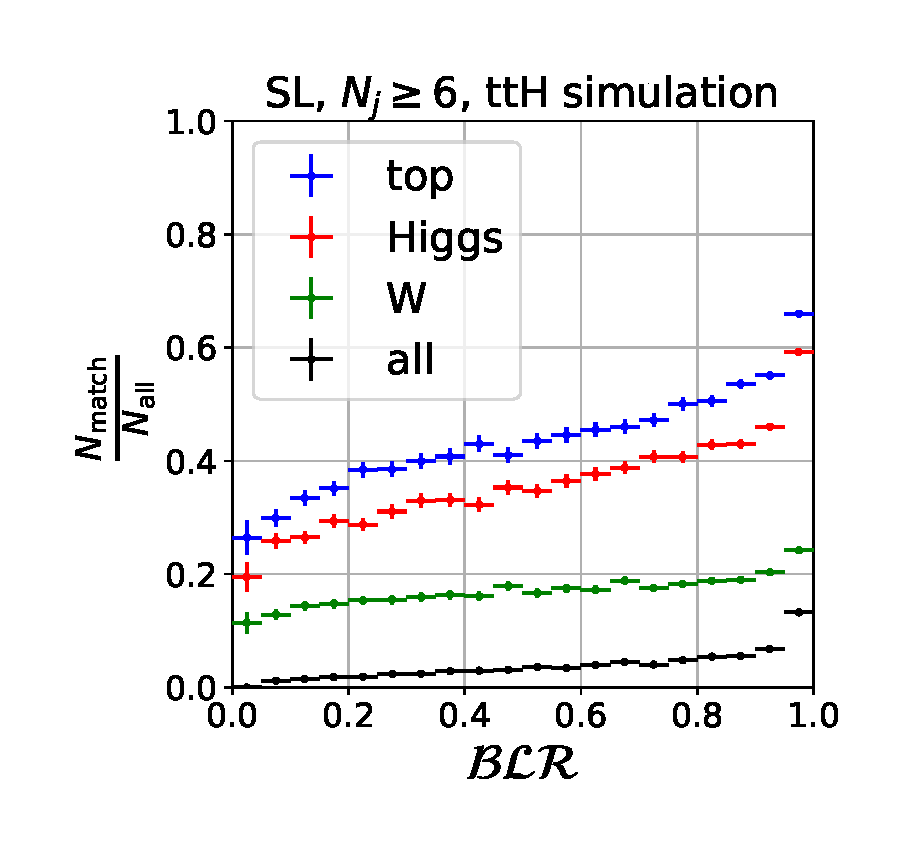
\includegraphics[width=0.5\textwidth]{figures/blr_matching.pdf}} 
\subfloat[Fraction of matched events with correct tagging.]{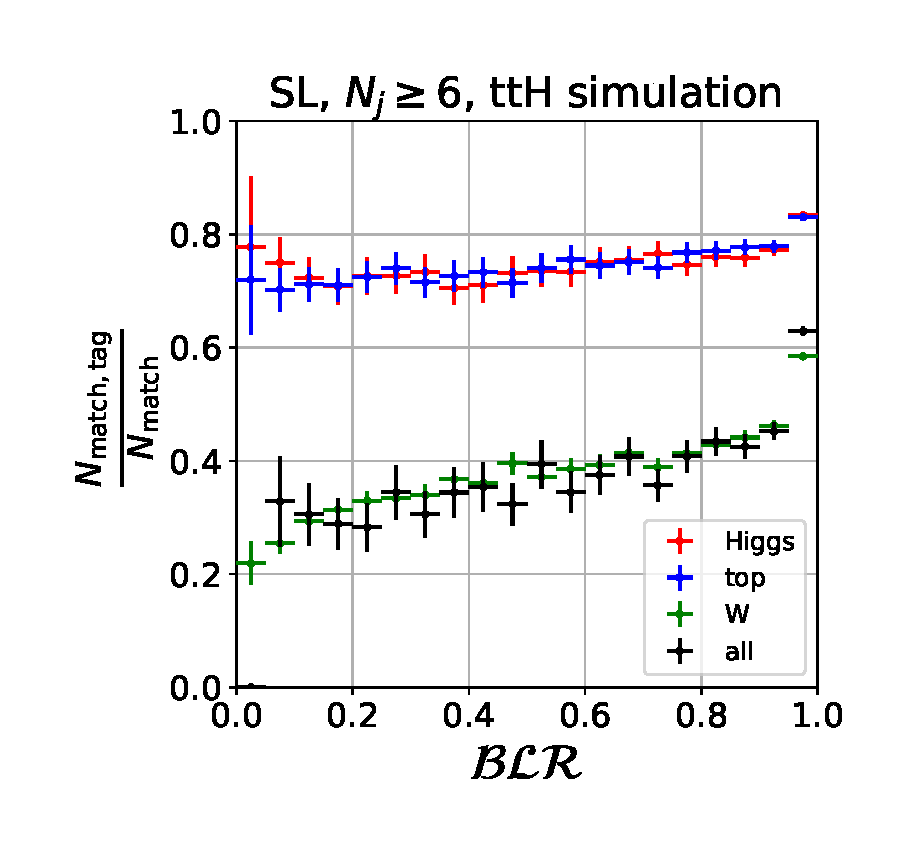
\includegraphics[width=0.5\textwidth]{figures/blr_matching_tag.pdf}}\\
\caption[Fraction of events with correct matching to the hard process]{Estimation of the fraction of events where the bottom quarks from the top quark, the Higgs boson and the light quarks from the W boson are reconstructed as jets in the final state on (\textbf{a}). We study the event-level b~tagging efficiency on (\textbf{b}), where we plot the fraction of events where the highest-likelihood permutation correctly assigned the bottom quarks to jets with respect to all events where the quarks were reconstructed as jets without considering tagging.}
\label{fig:blr_matching}
\end{centering}
\end{figure}
 
The likelihood ratio as defined here ignores the differences in~$f(\xi_k | \mathrm{b})$~and~$f(\xi_k | \mathrm{c})$, meaning that in the case of~$\mathrm{W} \rightarrow \mathrm{c}\bar{\mathrm{s}} (\bar{\mathrm{d}})$~decays, the discriminator is suboptimal. We have investigated extending this likelihood to also account for the possibility of such decays by a straightforward extension to $\mathcal{BL}(\vec{\xi} | M\mathrm{b}~1\mathrm{c})$. However, we have found that the additional combinatorial complexity suppresses any increased discrimination power and further progress would likely require methods that are better able to deal with the combinatorial problem using additional information, for example jet kinematics. We use this b~tagging likelihood ratio as a discriminator between the various~\ttbar+jets sub-processes, as well as to select the bottom quark candidates in the application of the MEM, as described in~\cref{sec:mem_application}. We have additionally studied whether switching to the new combined multivariate b~tagging algorithm (cMVAv2) introduced in~\cref{sec:btagging} would improve the analysis. Since the irreducible \ttbb\xspace background contains the same number of b~jets as the \ttHbb\xspace signal, improved b~tagging can only reduce contribution from the background components with light or charm quarks, which are inherently less problematic than \ttbb. We find that although there is a small increase in the signal rate by switching the b~discriminator, it is not sufficient to motivate a re-optimisation of the analysis at this stage. 

\subsubsection{B~discriminator shape calibration}
As we have used the detailed b~discriminator shape information in constructing the b~tagging likelihood ratio, we must experimentally calibrate the full range of this observable using data. This is accomplished by deriving a reweighting factor between data and simulation that depends on the jet b~discriminator value, jet kinematics and flavour using a tag-and-probe method. In this approach, the tag jet is required to pass the medium operating point that has been described earlier and the discriminator distribution of the probe jet is corrected by reweighting the MC simulation. In order to extract the weight for the b jets, the procedure relies on dilepton~\ttbar+jets events with the contribution from light jets and backgrounds subtracted using simulation, whereas for the scale factor for light jets, Z+jets events are used. The procedure is iterative, as the scale factor for light jets is required for the extraction of the b jet scale factor and vice versa~\cite{CMS:2013sea,CMS-PAS-BTV-15-001}. The systematic uncertainties from this reweighting method are described in~\cref{sec:systematic_unc}.

\subsubsection{Missing transverse energy}
The leptonic decays of the W boson produce neutrinos, which are only partially reconstructed by the detector as \MET, defined as the negative sum of all the momenta of the reconstructed particles in the transverse plane. In the SL channel, we can directly associate the~\MET~with the transverse momentum of the neutrino through the modelling of the recoil as described in~\cref{sec:transfer_functions} whereas in the DL channel, only the total momentum of both neutrinos is constrained by the \MET.

\section{Analysis}
\label{sec:analysis}
\subsection{Event selection and categorisation}
\label{sec:event_selection}

First, the large multi-jet QCD background is reduced to negligible levels by requiring that at least one of the top quarks in the~\ttHbb\xspace process decays leptonically. We divide events into two exclusive lepton categories: SL and DL, based on the multiplicity of the reconstructed charged leptons passing the quality cuts described in~\cref{sec:object_id_lep}. This is achieved by vetoing events with any additional leptons passing loosened quality criteria. We further suppress the $\gamma^*$ background by requiring~$m_{\ell\ell} > 20\GeV$~and Z+jets in the DL categories and reject events around the resonant Z boson peak with~$76\GeV < m_{\ell\ell} < 106\GeV$, where $m_{\ell\ell}$~is the invariant mass of the dilepton system. Furthermore, the leptons are required to have opposite charge. In the DL same-flavour categories, we require~$\MET > 40\GeV$. We do not explicitly distinguish between cases where the top quark decays to~$\mathrm{\tau}$~leptons, although these events can still pass the selection in case the~$\mathrm{\tau}$~lepton decays leptonically and are considered as signal.

Events from \ttHbb\xspace have a large number of jets and b~tags compared to the V+jets backgrounds. Therefore, we require the presence of at least four jets passing the quality criteria (\cref{sec:object_id_jets}), out of which at least three must be b~tagged according to the medium working point (\cref{sec:object_id_btag}). This brings us to the~\ttbar~dominated region, where we further distinguish between six categories in the SL channel
\begin{itemize}
\item~$\geq$6 jets, $\geq$4 b~tags;\ 5 jets,\ $\geq$4 b~tags and 4 jets, 4 b~tags, that are the most signal-enriched categories,
\item~$\geq$6 jets, 3 b~tags;\ 5 jets, 3 b~tags and 4 jets, 3 b~tags, that contain a significant amount of \ttcc~and \ttbb,
\end{itemize}
and two categories in the DL channel
\begin{itemize}
\item~$\geq$ 4 jets, $\geq$ 4 b~tags,
\item~$\geq$ 4 jets, 3 b~tags,
\end{itemize}
resulting in a total of eight exclusive categories, as shown in~\cref{fig:tth_pies}.

\begin{figure}
\begin{centering}
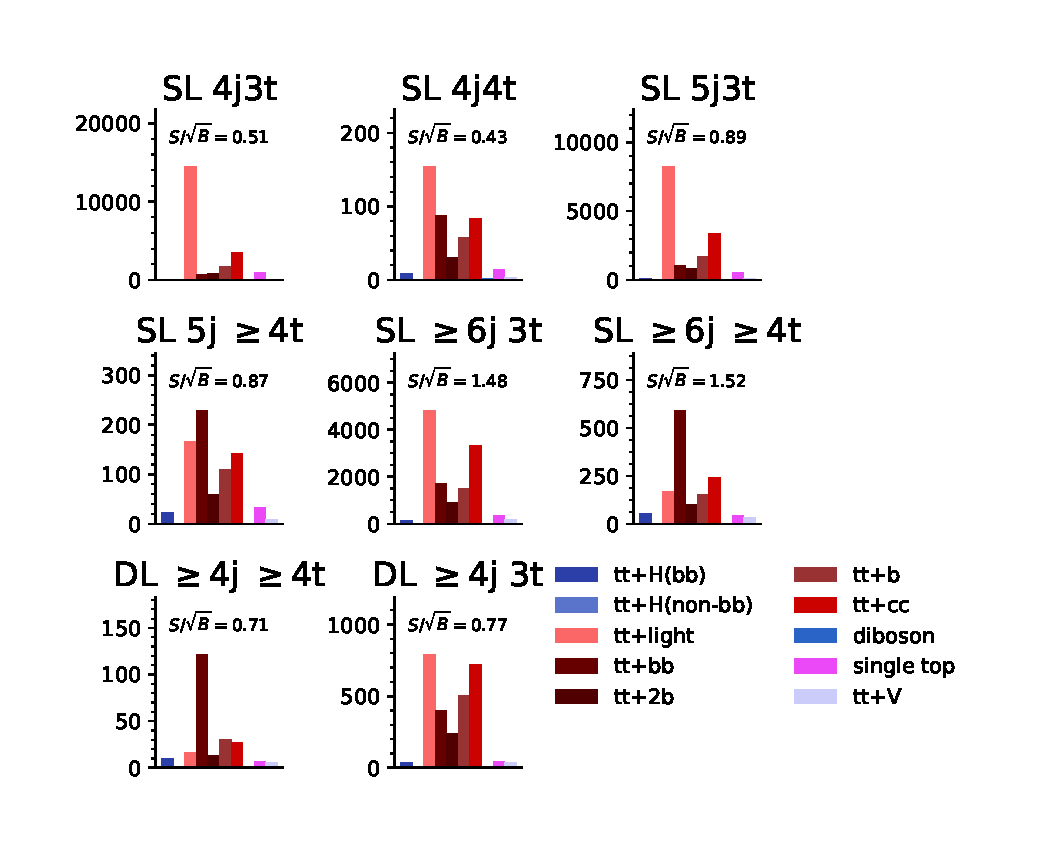
\includegraphics[width = 1.0\textwidth]{figures/tth/pies.pdf}
\caption[The expected signal and background yields in the analysis categories]{The expected signal and background yields in the semileptonic (SL) and dileptonic (DL) analysis categories. We also show the expected signal over background ratio $S / \sqrt{B}$. As can be seen, the expected signal yield is quite low compared to the predicted background, even in the most high-purity categories of SL $\geq6$~jets (j), $\geq4$~b~tags (t) and DL $\geq4$~jets, $\geq4$~b~tags.}
\label{fig:tth_pies}
\end{centering}
\end{figure}

We use the MEM as a \ttHbb\xspace to~\ttbb~discriminator in the categories with~$\ge 4$~b~tags as these categories are enhanced in the signal fraction and have been shown to have an excellent discriminator performance for the MEM. The categories with three b~tags are retained as control regions where we determine the \ttbar+jets background rates by fitting the b~tagging likelihood discriminator. We now turn to the description of the signal extraction using a template fit. 

\subsection{Signal extraction}
\label{sec:mem_application}
The likelihood discriminant based on b~tagging enhances the~\ttbar+heavy flavour component, but the cross-section of~\ttbb~is still an order of magnitude larger than that of \ttHbb. Furthermore, we cannot directly reconstruct the resonant peak of the \Hbb~decay as a natural discriminant between the signal and non-resonant background. Even though the width of the SM Higgs boson is relatively small compared to detector resolution ($\Gamma_{\mathrm{SM}} = 4.07 \times 10^{-3}\GeV$), the presence of multiple additional bottom quarks due to top decay in the final state creates a combinatorial self-background in the form of an ambiguity in choosing the candidate jets for the \Hbb~decay.

An estimator for the Higgs candidate invariant mass, built from randomly selected jet pairs, results in a much broader distribution compared to experimental resolution, whereas choosing the pair of jets that would give a mass closest to~$m_H$~would cause also the background to exhibit a signal-like peak.

Therefore, we use the MEM discriminant, introduced in~\cref{sec:mem}, to compute theory-motivated weights~$P_{\ttHbb}$~and~$P_{\ttbb}$~for each candidate event. We construct a signal-to-background discriminant~$P_{\mathrm{s/b}}$~based on the likelihood ratio of these weights, as described in~\cref{sec:mem_performace}, which based on the Neyman-Pearson lemma, described in~\cref{sec:test_statistic}, is the optimal test statistic between the signal and background hypotheses.

As an improvement over the search for~\ttHbb\xspace performed by the CMS experiment in Run I~\cite{Khachatryan:2015ila}, we use the MEM discriminant also in categories which are not fully reconstructed, but still contain a large amount of signal, namely five-jet and four-jet categories in the SL channel. The details of the additional MEM hypotheses are described in~\cref{sec:event_interpretation}. We list the discriminants that have been used in the different categories in~\cref{tab:cat_discriminant}. 


\begin{table}[h!]
\begin{center}
\caption[The analysis categories for the~\ttHbb\xspace analysis.]{The analysis categories and the discriminators used in those categories.}
\label{tab:cat_discriminant}
\begin{tabular}{c|c}
\hline
category & discriminant \\
\hline
SL~$\geq6$~jets,~$\geq4$~tags & MEM SL~$2_{\mathrm{W}} 2_{\mathrm{h}} 2_{\mathrm{t}}$~\\
SL~$\geq6$~jets,~$3$~tags & The b~tagging likelihood ratio \\
\hline
SL~$5$~jets,~$\geq4$~tags & MEM SL~$1_{\mathrm{W}} 2_{\mathrm{h}} 2_{\mathrm{t}}$~\\
SL~$5$~jets,~$3$~tags & The b~tagging likelihood ratio \\
\hline
SL~$4$~jets,~$\geq4$~tags & MEM SL~$0_{\mathrm{W}} 2_{\mathrm{h}} 2_{\mathrm{t}}$~\\
SL~$4$~jets,~$3$~tags & The b~tagging likelihood ratio \\
\hline
DL~$4$~jets,~$\ge4$~tags & MEM DL~$2_{\mathrm{h}} 2_{\mathrm{t}}$~\\
DL~$4$~jets,~$3$~tags & The b~tagging likelihood ratio\\
\hline
\hline
\end{tabular}
\end{center}
\end{table}

We use the~\ttbb~matrix element as a representative background diagram in all categories. This gives the best separation in the most signal-rich categories against~\ttbb~and is further motivated by simulation, where we see that using this process as background still achieves a high rate of separation in categories enriched in other \ttbar+jets sub-processes. As an optimisation, considering additional background hypotheses in different categories in the future is expected to improve the signal-to-background discrimination at the cost of computational complexity.

As the b~tagging likelihood ratio method is optimised to identify the set of jets that are most compatible with arising from four bottom quarks, we further augment the MEM by assuming that the bottom quarks need to be considered only among those four jets, as explained in~\cref{sec:event_interpretation}. This means that we have exactly four candidates for the bottom quarks from \Hbb~and~$\mathrm{t} \rightarrow \mathrm{W} \mathrm{b}$~decay, whereas the remaining jets are assumed to arise from~$\mathrm{W} \rightarrow \mathrm{q} \mathrm{q}'$~or from unspecified sources. 

Both of these discriminators are complex multivariate functions based on quantities which have significant modelling uncertainties affecting the shapes of the distributions. Therefore, a realistic description and propagation of the systematic uncertainties is crucial in the interpretation of data.

\subsection{Systematic uncertainties}
\label{sec:systematic_unc}
Among the experimental uncertainties, the dominant ones are uncertainties on the jet energy scale and resolution corrections (\cref{sec:jec_unc}) and the reweighting of the b~tagging discriminant (\cref{sec:btag_unc}). Both of these can affect the predicted yields of all the processes, since they change the selection efficiency, as well as the shapes of the final discriminants. In case the source of an uncertainty is the same across several categories, the nuisance parameters associated with the uncertainties are treated as fully correlated, otherwise, the uncertainties are treated as uncorrelated in the fit.

Concerning theory systematics, the uncertainties on the modelling of the \ttbar+jets background are the ones with the largest impact on the measurement. As introduced in~\cref{sec:ttbar_subprocesses}, the~\ttbar+jets \texttt{POWHEG} model we currently use in the analysis treats the~\ttbb~process only at leading order accuracy, where the~$\mathrm{b}\bar{\mathrm{b}}$~pair is generated from gluon splittings using a parton shower, such that we have considerable additional theoretical uncertainties on the modelling of \ttbb, as will be described in~\cref{sec:theory_unc}.

We give a detailed overview of the most important experimental and theoretical uncertainties along with their estimation in the next sections. The full list of systematic uncertainties along with the assumed priors is shown in~\cref{tab:systematic_uncertainties_prior}.

\begin{table}[h!]
\begin{center}
\begin{tabular}{c|cccc}
\hline
uncertainty & normalisation & shape & processes & prior \\
\hline
JES (26 sources) & yes & yes & all & Gaussian, $<5\%$ \\
JER & yes & yes & all & Gaussian, $<1\%$ \\
b~tagging (9 sources) & yes & yes & all & Gaussian, $0-20\%$ \\
pileup & yes & yes & all & Gaussian, $0-5\%$ \\
lepton ID & yes & yes & all & Gaussian, $\simeq1\%$ \\
lepton isolation & yes & yes & all & Gaussian, $\simeq1\%$ \\
luminosity & yes & no & all & log-normal, $2.4\%$ \\
limited MC statistics & no & yes & all & bin-by-bin Poisson \\
\hline
\ttbar+jets ISR, FSR & yes & partly & \ttbar+jets & log-normal, 0-15\% \\
\ttbar+jets tune, $h_{\mathrm{damp}}$ & yes & partly & \ttbar+jets & log-normal, 0-15\% \\
\ttbb~norm. & yes & no & \ttbar+jets & log-normal, 50\% \\
\ttb~norm. & yes & no & \ttbar+jets & log-normal, 50\% \\
\tttwob~norm. & yes & no & \ttbar+jets & log-normal, 50\% \\
\ttcc~norm. & yes & no & \ttbar+jets & log-normal, 50\% \\
PDF~(gg) & yes & no & \ttH, \ttbar+jets & log-normal, 4\% \\
PDF~(qq') & yes & no & W+jets & log-normal, 2\% \\
PDF~(qg) & yes & no & single top & log-normal, 3\% \\
$\mu_R$, $\mu_F$ scale & yes & yes & \ttbar+jets & Gaussian \\
scale uncertainties in norm. & yes & no & primarily \ttH & log-normal \\
\hline
\hline
\end{tabular}
\caption[Systematic uncertainties in the~\ttHbb\xspace analysis.]{Systematic uncertainties in the~\ttHbb\xspace analysis. We list whether a particular source of uncertainty changes the predicted normalisation of processes and whether it has an effect on the discriminator distributions, i.e. the shapes. For each uncertainty, we also show for illustrative purposes the size of the prior uncertainty in a relevant variable, e.g. jet momentum spectrum for JES, and the distributions used to model the nuisance parameters associated to each uncertainty. We further distinguish between experimental uncertainties, which affect all processes, and theoretical uncertainties that are specific to particular processes. Although the \ttbar+jets ISR, FSR, MC tune and $h_{\mathrm{damp}}$ modelling uncertainties affect also the discriminator distributions, due to limited MC simulation statistics, we only account for the normalisation effect as a function of jet multiplicity, as further described in~\cref{sec:theory_unc}, therefore these uncertainties are listed as having a partial effect on the shape.}
\label{tab:systematic_uncertainties_prior}
\end{center}
\end{table}

\subsection{Jet energy correction uncertainties}
\label{sec:jec_unc}
We apply jet energy scale (JES) and resolution (JER) corrections between data and simulation, as described in~\cref{sec:jes_calibration}. Thus, we need to understand the effect of the uncertainties on these corrections. In Run 2, we consider various uncorrelated sources of jet energy scale correction uncertainties with their corresponding correlations, as opposed to a single bulk JES uncertainty as was done for this analysis in Run I. This significant advancement has resulted from an improved modelling of the detector performance and better calibration techniques developed with more data. By treating the various sources of JES uncertainties independently, the assumptions that allow the profile likelihood fit to constrain the combined JES uncertainty significantly in Run I are thus relaxed and the final uncertainty is a more realistic estimate of the true uncertainty.

The magnitude and correlation of the uncertainties on JES and JER are determined in a dedicated CMS analysis and are provided as a vector of per-jet corrections with~$p_T$~and~$\eta$~dependent correlations~\cite{cms_jec_2017}. The most important groups of correction uncertainties are the following:

\begin{itemize}
\item Pileup offset, which results from extra energy deposited in jets from additional pp interactions within the same bunch crossing (in-time pileup) or due to the finite signal decay time in the calorimeters (out-of-time pileup). The uncertainty for this source results from the~$\eta$-dependent scale factor used to correct the offset distribution measured in simulation.
\item Relative~$\eta$-dependent corrections, which calibrate the forward regions of the detector with respect to the central region. Uncertainties of this type arise from jet energy resolution and from the modelling of initial and final state radiation (ISR+FSR).
\item Uncertainties on the absolute energy scale, which are derived using Z/$\gamma$+jet and multijet data. The energy scale uncertainties are driven by the muon momentum scale and the single pion response in the HCAL. Furthermore, the uncertainties in fragmentation are assessed in a comparison of the \texttt{PYTHIA} and \texttt{HERWIG++} MC models.
\item Uncertainties in the modelling of the detector response for jet flavour, which are assessed using simulation and are largest for gluon jets.
\item Finally, due to radiation damage, there is a residual time-dependent uncertainty in the scale corrections, which is estimated using dijet events in different run periods.
\end{itemize}

These five broad groups factorise into approximately 26 independent sources. In order to account for the JES scale uncertainties in the analysis, we propagate the uncertainties in jet energy scale and resolution corrections to the jet momenta and all the event-level observables that are derived from them, such as the jet and b~tag multiplicities, by changing the jet energy scales and resolutions by one standard deviation up and down from the nominal values. This is done separately for all the sources so that we can fully account for the correlations between the various sources. Thus, we are able to account for both the changes in efficiency (normalisation) and discriminator shape in the final analysis categories. We find that the normalisation effects are of the order of 0-4\% for all JES and JER sources for the SL channel and around 0-1\% in the DL channel, with the largest variations resulting from the jet flavour response modelling.

In order to propagate the uncertainty to high-level multivariate observables such as the MEM discriminator, they need to be recomputed using the varied jets. We use the approximate MEM vector integration technique for this as described in~\cref{sec:mem_uncertainties}. In addition to uncertainties in the jet energy scale corrections, we also consider uncertainties on the jet energy resolution corrections. In the tracker acceptance region, the relative JER uncertainty is around 2-4\%, depending on the jet pseudorapidity $|\eta|$. The JER uncertainty is propagated by shifting the JER scale factor up and down by one standard deviation corresponding to the uncertainty, thus it is fully deterministic. The overall effect of the JES and JER uncertainties on the leading jet transverse momentum distribution is shown in~\cref{fig:jec_pt_effect}. These uncertainties will mostly affect the predicted yields in our final analysis categories.

\begin{figure}
\begin{centering}
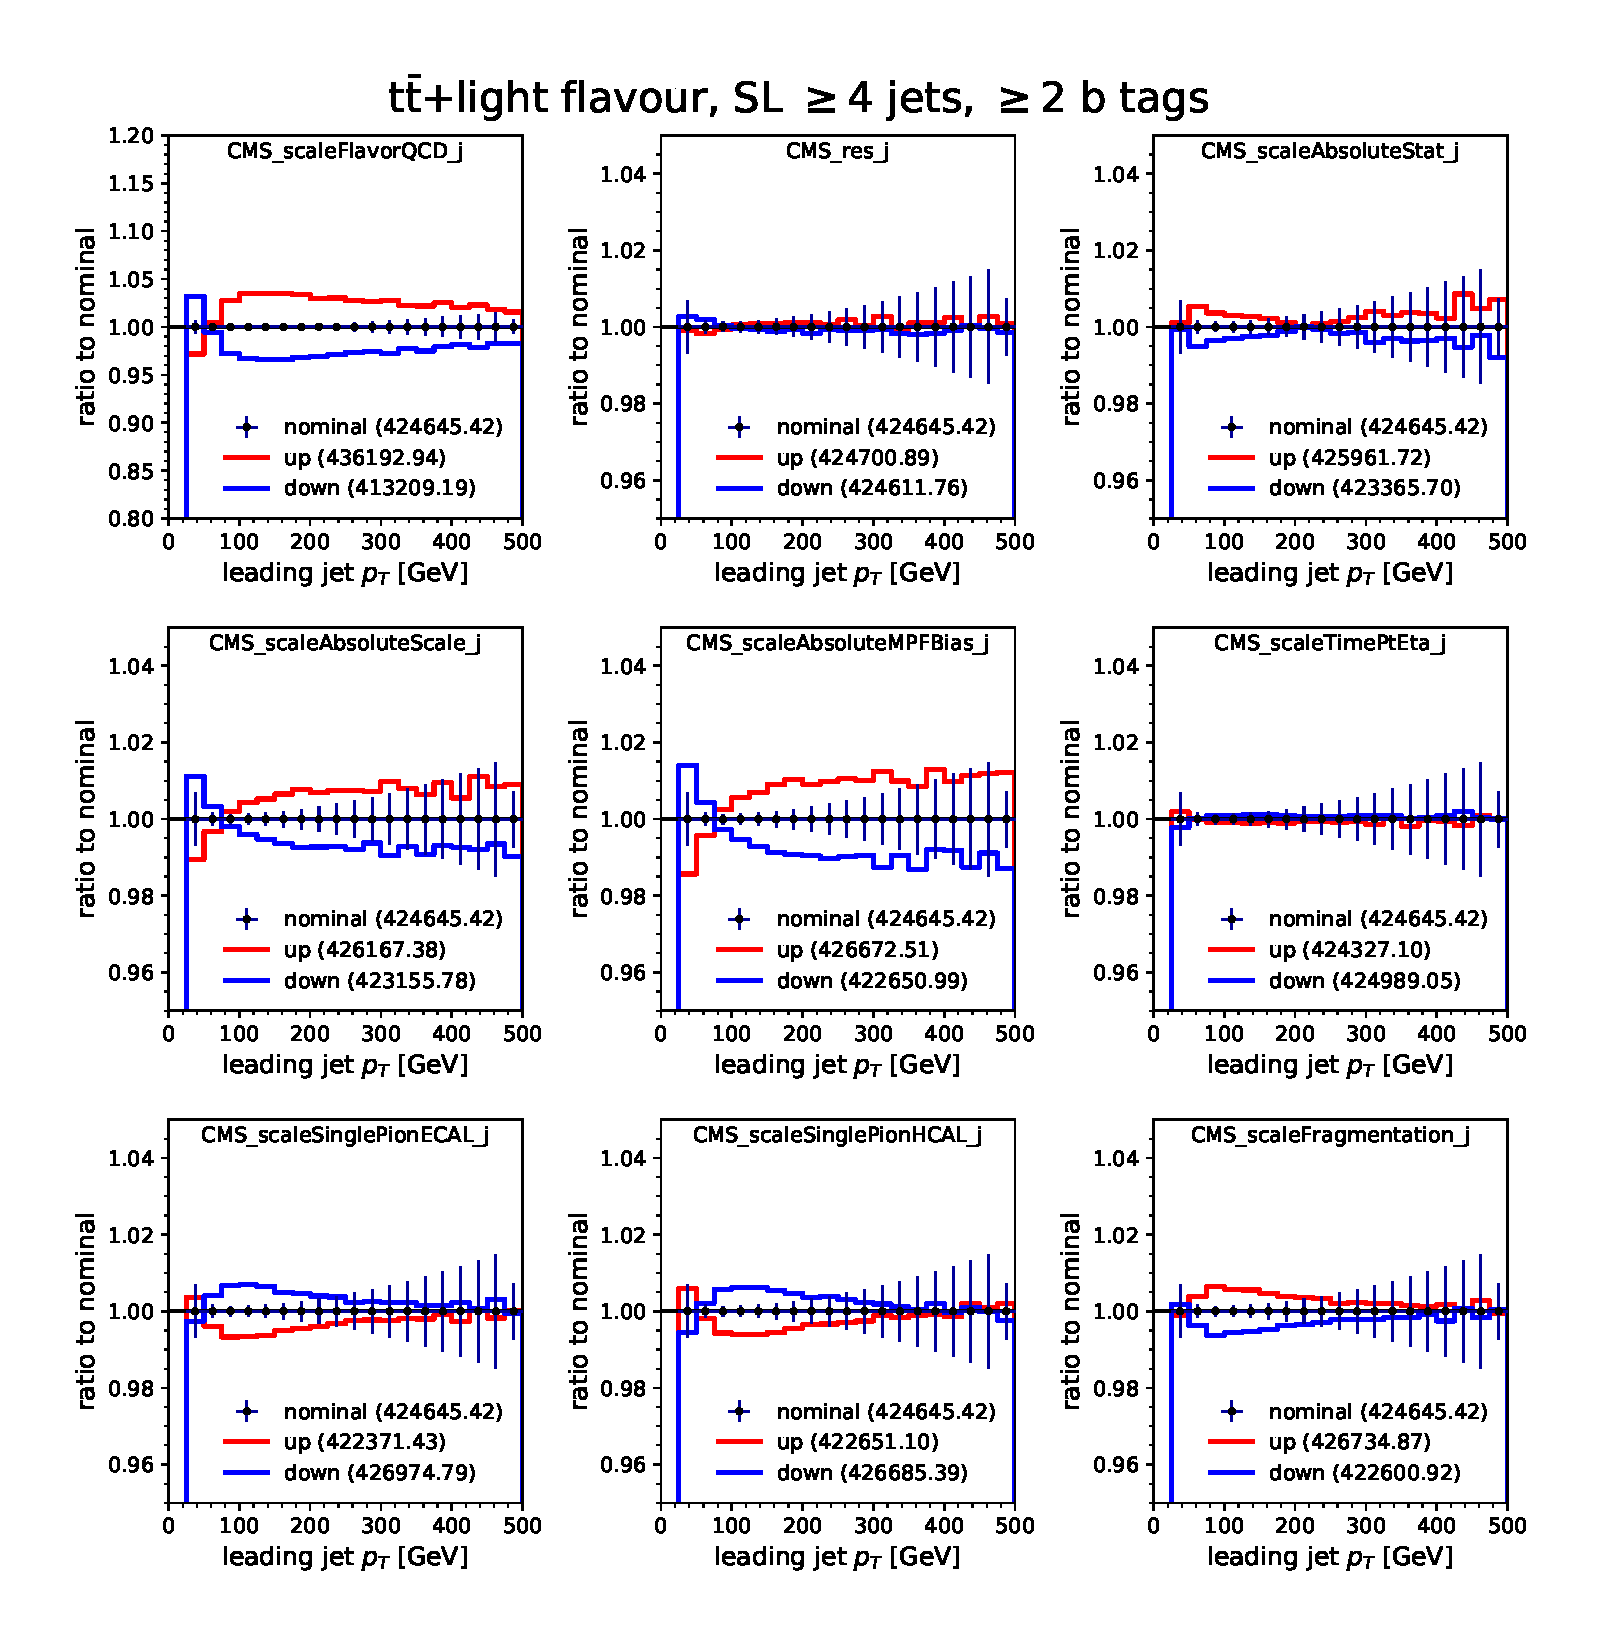
\includegraphics[width=1.0\textwidth]{figures/tth/sl_jge4_tge2_jec_unc.pdf}
\caption[Effect of jet energy corrections.]{The effect of jet energy corrections on the leading jet transverse momentum distribution. In the top row, we show the distribution under variations of the flavour composition (left), jet energy resolution (middle) and the statistical uncertainties in the absolute scale determination (right). In the middle row, we show the overall uncertainty from the absolute scale variation (left), the uncertainty arising from the corrections derived using the missing momentum projection fraction (MPF, middle) and the time-dependent momentum scale variation (right). On the bottom row, we show the uncertainties in the single pion response in the ECAL (left), HCAL (middle) and the fragmentation model (right). In general, we see that the variations are within a few percent of the nominal, with the largest effect from the uncertainties on the flavour response (top left).}
\label{fig:jec_pt_effect}
\end{centering}
\end{figure}

\subsection{b~tagging systematic uncertainties}
\label{sec:btag_unc}
Due to the high expected number ($\geq4$ in the signal regions) of b~tagged jets in the~\ttHbb\xspace final state, this analysis is sensitive to uncertainties in b~tagging, which arise from the MC modelling of the input variables used in the construction of the multivariate b~tagging discriminator. As we have described in~\cref{sec:object_id_btag}, we correct for mis-modelling in the b~tagging discriminator shape using a tag and probe method, such that the detailed b~discriminator shape can be used in further template fitting. The effect of this shape correction is shown in~\cref{fig:tth_btag_rew}, where we see that the correction improves the description by the MC, with the corrected distribution agreeing with data within the systematic uncertainties.

\begin{figure}
\begin{centering}
\subfloat{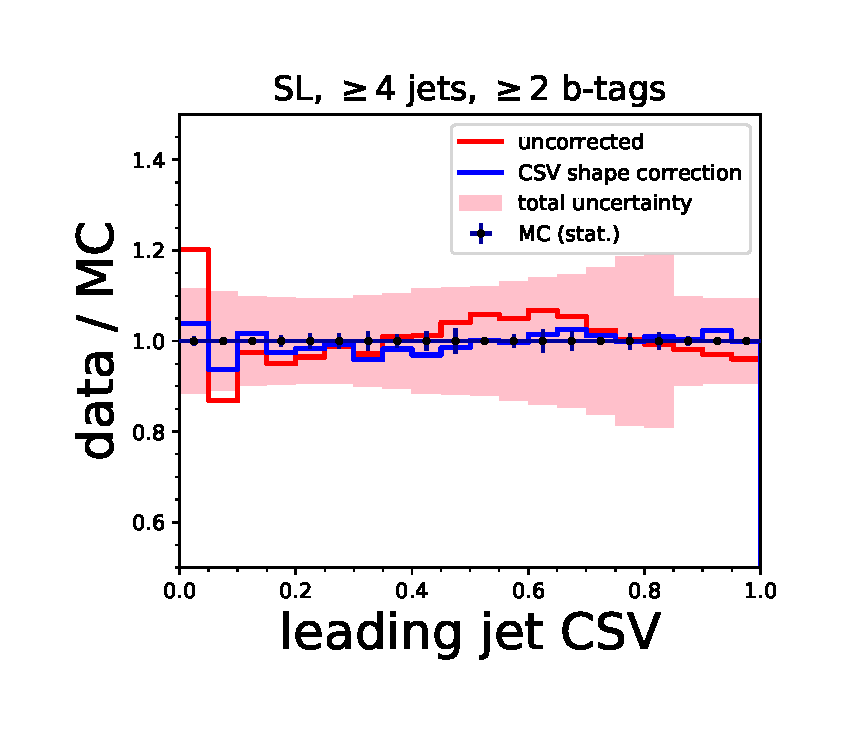
\includegraphics[width = 0.5\textwidth]{figures/tth/sl_jge4_tge2_csv.pdf}}
\subfloat{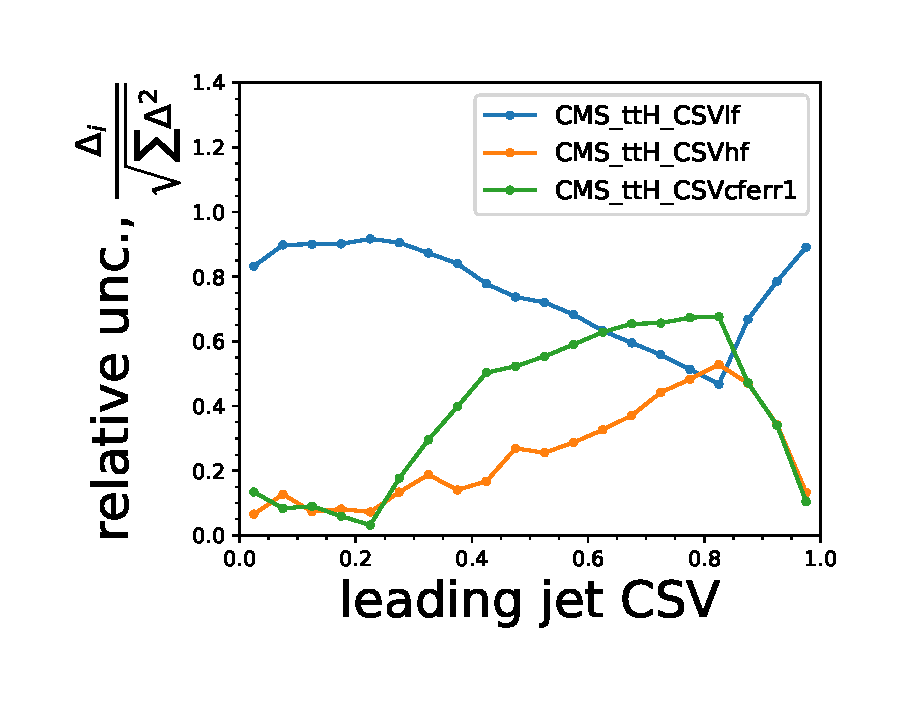
\includegraphics[width = 0.5\textwidth]{figures/tth/sl_jge4_tge2_csv_rel.pdf}}
\caption[b~tagging reweighting and uncertainty]{The effect of the b~tag reweighting on the MC modelling (left). We see that the b~tag reweighting technique improves the modelling from the nominal case (red) to the corrected case (blue), with the total uncertainties (pink) over-covering the difference. On the right plot, we see that the overall uncertainty band consists mainly of the light flavour (blue), charm flavour (green) and heavy flavour (orange) uncertainty components.}
\label{fig:tth_btag_rew}
\end{centering}
\end{figure}

The uncertainties of this correction include the propagation of jet energy scale uncertainty, which affects the determination of the correction through changes in efficiency and the discriminator value. Furthermore, simulation is used to subtract the non-relevant jet flavour components in determining the scale factor for bottom (light) jets. For the scale factor for light jets, the fraction of bottom (charm) jets is varied within 20\% of the MC prediction in the Z+jets simulation used to determine the scale factors. Similarly, for the extraction of the b jet scale factor, the light flavour component in the \ttbar+jets dileptonic sample arises from additional radiation and is estimated to be $\simeq20\%$~\cite{CMS-PAS-BTV-15-001}.

As the b discriminator scale factor is determined in bins of the discriminator value, statistical fluctuations in bins with a low number of data and simulated events introduce an uncertainty on the final scale factor. This uncertainty is only significant in case the size of the fluctuations varies systematically over the b discriminant range. Since the discriminator has a roughly monotonous increasing (decreasing) shape for b jets (light jets), this condition is fulfilled. The statistical uncertainties are accounted for by a sum of polynomials of first and second order, where the nuisance parameter is the overall scale of the distortion.

There is currently no dedicated b discriminator scale factor for charm jets, therefore, the uncertainties on the charm flavour scale factor are assumed to be twice as large as for the b jet scale factor, with the  scale factor being unity. We propagate the uncertainties from b~tagging in the form of a set of per-event weights, which are determined from the individual per-jet weights that are used to correct the jet b discriminator distributions. The uncertainties on the b~discriminator scale factor result in both normalisation effects due to acceptance changes, which can be up to 20\% in some cases, and shape effects on the templates. An example of the effect of b~discriminator uncertainties is shown in~\cref{fig:tth_btag_unc}. 


\begin{figure}
\begin{centering}
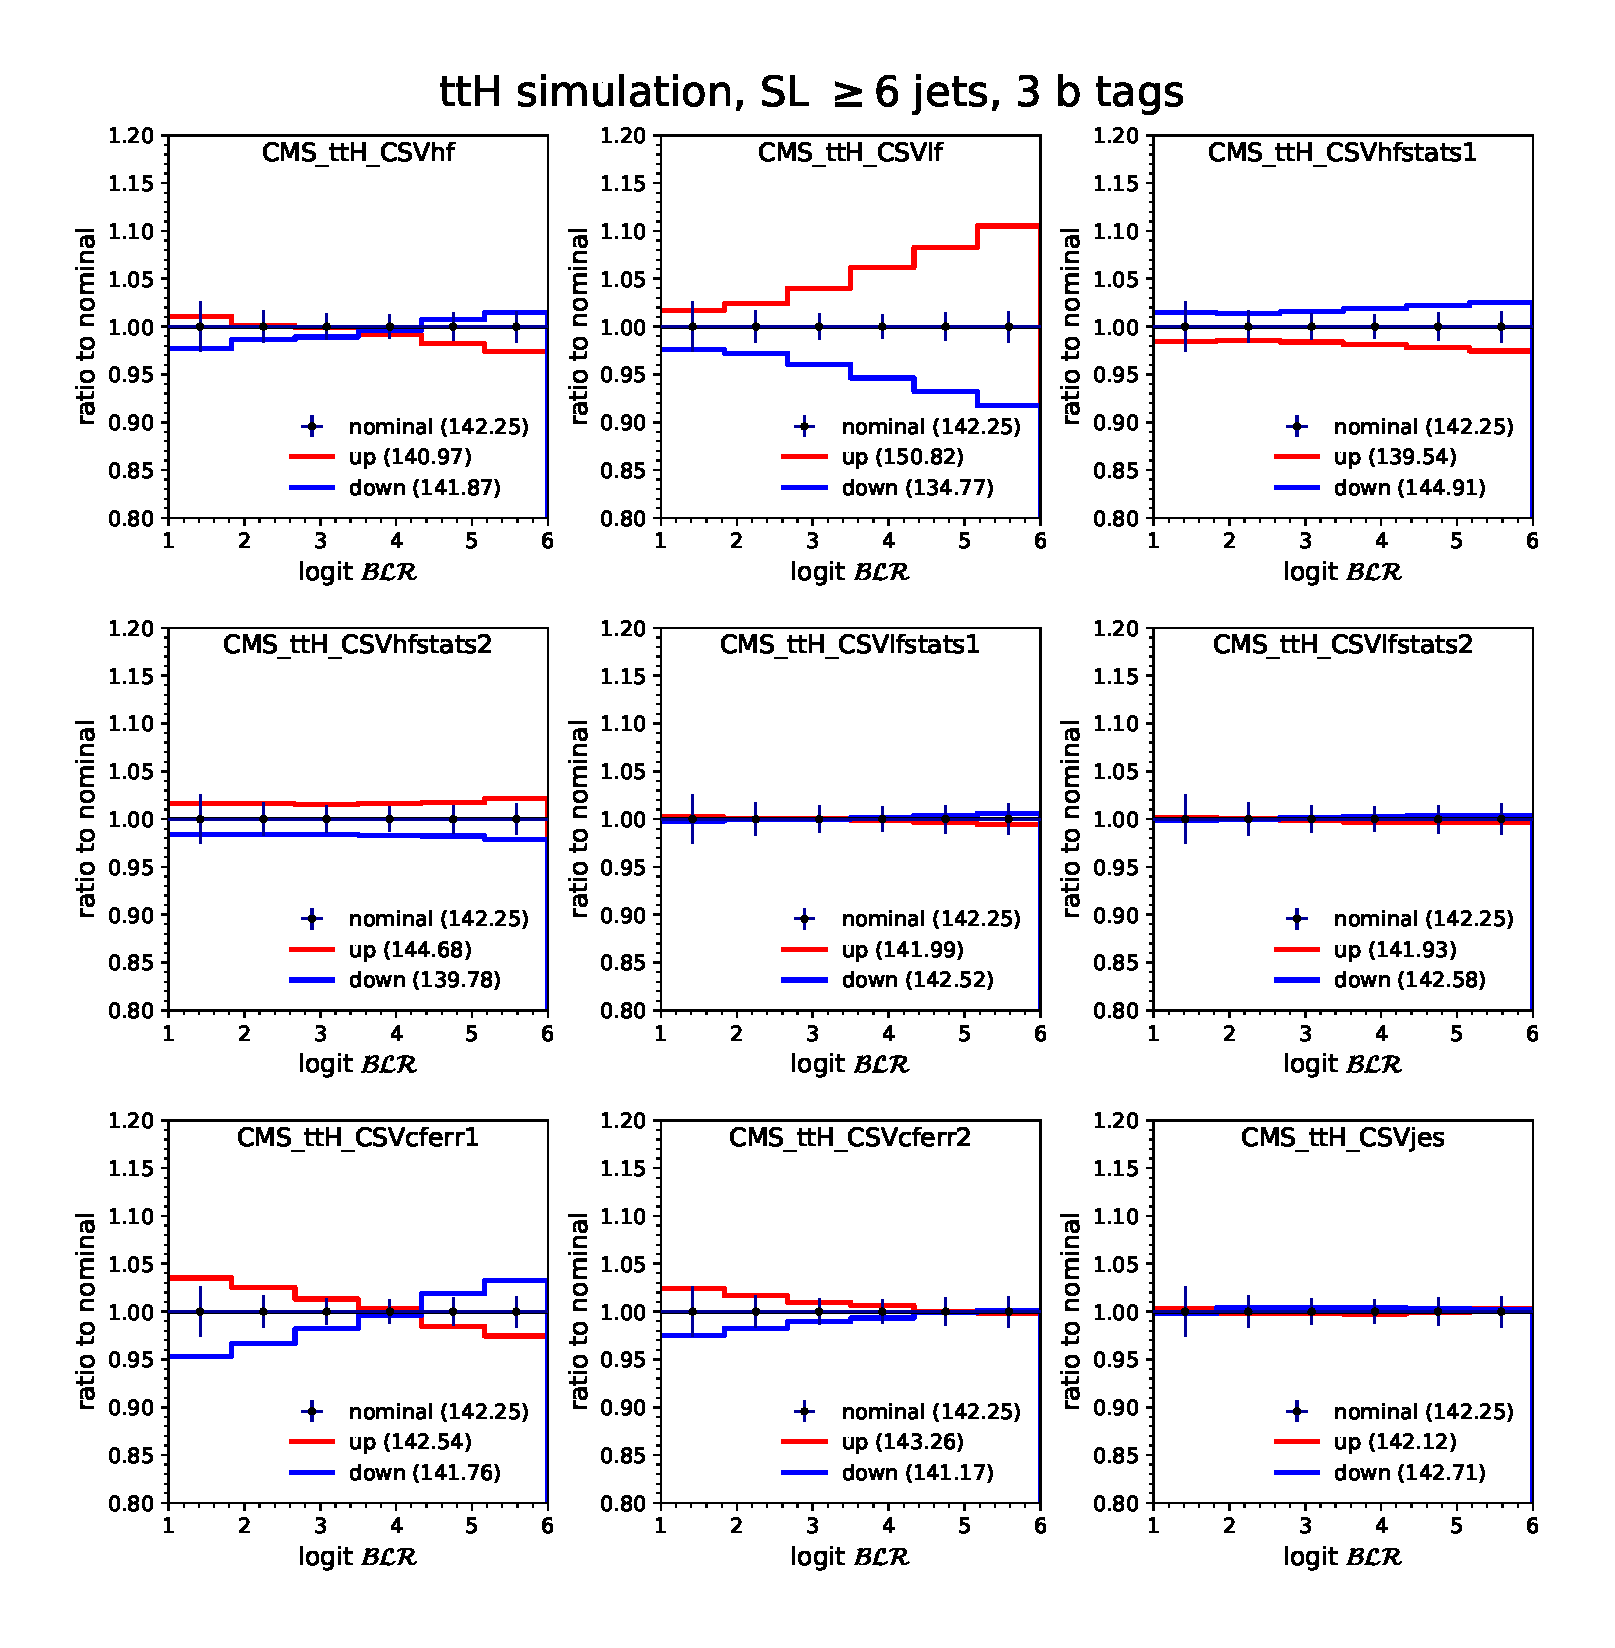
\includegraphics[width = 1.0\textwidth]{figures/tth/sl_jge6_t3_blr_unc.pdf}
\caption[The effect of b~tagging uncertainties on the b~tagging likelihood ratio.]{The effect of b~tagging uncertainties on the b~tagging likelihood ratio distribution for the~\ttHbb~sample. In the top row, we show the effect of the heavy flavour (left), light flavor (center) and the linear heavy flavour distortion from statistical uncertainties (right). In the middle row, we show the effect of the quadratic distortion on the heavy flavour scale factor from statistical uncertainties (left) and the linear and quadratic uncertainties on the light flavour scale factor (middle, right). In the bottom row, we show the uncertainties for the charm flavour jets (left, middle) and the uncertainty on the scale factor arising from the propagation of JES uncertainties. These templates are derived in the SL $\geq6$ jet, three b~tag category on \ttH~simulation.}
\label{fig:tth_btag_unc}
\end{centering}
\end{figure}

\subsection{Other experimental systematic uncertainties}
We also assess the effect of uncertainties in the lepton identification, isolation and trigger selection, which may have different efficiencies in data and simulation and are thus corrected using scale factors. For muons, we assign a~$1\%$~normalisation uncertainty for the lepton ID,~$1\%$~for isolation and~$0.5\%$~for the effect of highly-ionising particles, on top of the statistical uncertainties on the muon scale factor~\cite{CMS:2017_mu_sf}. For electrons, we use~$p_T$~and ECAL supercluster~$\eta$-dependent scale factor uncertainties derived using a tag-and-probe method, which are generally below~$1\%$~\cite{CMS:2017_ele_sf}.

As the pileup profile in simulation is corrected to data using a pileup-dependent scale factor, we estimate the uncertainty in the pileup correction by varying the minimum bias cross section from~$\sigma = 69.2$~mb by~$4.6\%$, corresponding to the uncertainty in the number of interactions in minimum bias events from luminosity and cross section\cite{CMS:2017_pu_weight_twiki}. This results in both a normalisation and shape effect in the predicted templates.

Furthermore, the uncertainty on the total integrated luminosity is estimated to be~$2.4\%$~using cluster counting in the pixel detector and affects the normalisation of all processes in a correlated way~\cite{CMS:2017sdi,CMS:2017_lumi}.

\subsection{Theoretical uncertainties}
\label{sec:theory_unc}
The most important theoretical uncertainties arise from the modelling of the \ttbar+heavy flavour processes, namely \ttbb, \tttwob, \ttb~and \ttcc. Currently, it is not possible to isolate a pure~\ttbb~control region which would not contain a significant amount of~\ttHbb\xspace and thus this background cannot be determined directly from data. Although inclusive measurements of the~\ttbb~cross-section have been carried out in CMS~\cite{Sirunyan:2017snr} with $\sigma_{\ttbb}$ determined with a $\simeq 35\%$ relative accuracy, these analyses treat \ttHbb\xspace as an irreducible background and thus cannot directly be used to set the prior uncertainties in our analysis. On the other hand, NLO estimates for the inclusive cross-section of $\sigma_{\ttbb}$ have residual theoretical uncertainties at the level of $\simeq 20\%$~\cite{Bredenstein:2010rs}, with important differences between alternative models in the differential predictions. Therefore, we assign a conservative 50\% normalisation uncertainty on all the \ttbar+heavy flavour processes, which is assumed to be uncorrelated across the aforementioned sub-processes. Correlating these uncertainties would reduce their overall impact. Effectively, this allows us to use the data in the control regions to determine the best fit values of the cross-sections for the \ttbar+heavy flavour processes in a consistent way with the extraction of the signal strength modifier. We do not use additional extrapolation uncertainties for the \ttbar+jets processes between the control and signal regions, as the combined fit provides a consistent framework for determining the best-fit estimates given the data.

The inclusive cross sections of all involved signal and background processes are known to at least NLO accuracy, with a 4\%~renormalisation and factorisation scale uncertainty and a 4\% PDF uncertainty on the gluon-gluon dominated production of~\ttbar~+jets. Shape uncertainties from PDF variations are found to be negligible and thus not considered further in the analysis. We use MC simulation to estimate the shape effect of the renormalisation and factorisation scale ($\mu_R$ and $\mu_F$) on the final discriminant shape by changing the nominal values of $\mu_R$ and $\mu_F$ by 0.5 (2.0) for the down (up) variation. This is achieved using the embedded matrix-element dependent weights in the MC simulation. The effect of these variations is illustrated in~\cref{fig:tth_scaleme} and is generally small on the final observables, but has a significant effect on the jet multiplicity and transverse momentum distributions.

\begin{figure}
\begin{centering}
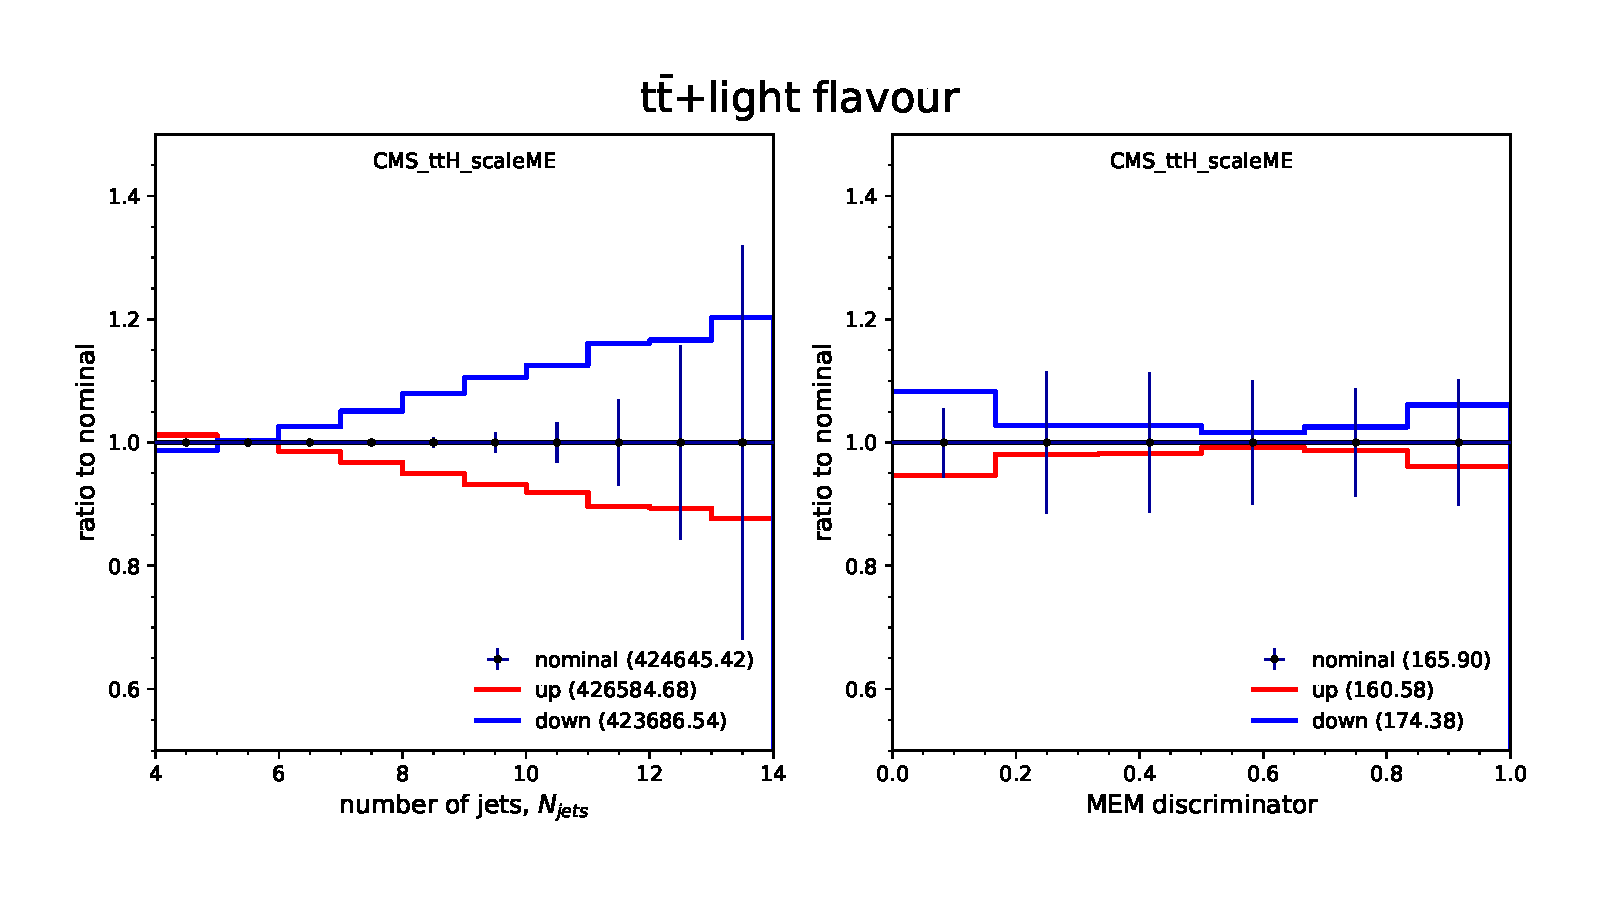
\includegraphics[width=0.8\textwidth]{figures/tth/scaleME_unc.pdf}
\caption[The effect of $\mu_r$ and $\mu_f$ variations.]{The effect of the renormalisation and factorisation scale variations ($\mu_r$ and $\mu_f$) on the modelling of the jet multiplicity (left) in the SL $\geq4$jet, $\geq2$~b~tag inclusive region and the MEM discriminator (right) in the SL $\geq6$jet, $\geq4$~b~tag signal region. While the effect of the scale changes is normalised to be shape-changing in the inclusive region, it can introduce migrations between jet-tag bins among the final categories. These distributions are derived using \ttlf~simulation.}
\label{fig:tth_scaleme}
\end{centering}
\end{figure}

For the parton shower uncertainties, in particular the effects of ISR and FSR, we have limited MC simulation samples that can only be used to determine the overall effect on normalisation, whereas the shape distortions on the distributions are generally consistent with no change. These background modelling uncertainties primarily affect jet kinematics and thus the number of reconstructed jets in the final state. Therefore, we model these uncertainties through per-subprocess normalisation factors that depends on the jet multiplicity, with the magnitude of the uncertainties generally between 5-15\%, as seen in~\cref{fig:tth_ttjets_modelling}. The overall normalisation and shape effect of the most important shape changing uncertainties is shown in~\cref{fig:tth_uncertainties_effect}.

\begin{figure}
\begin{centering}
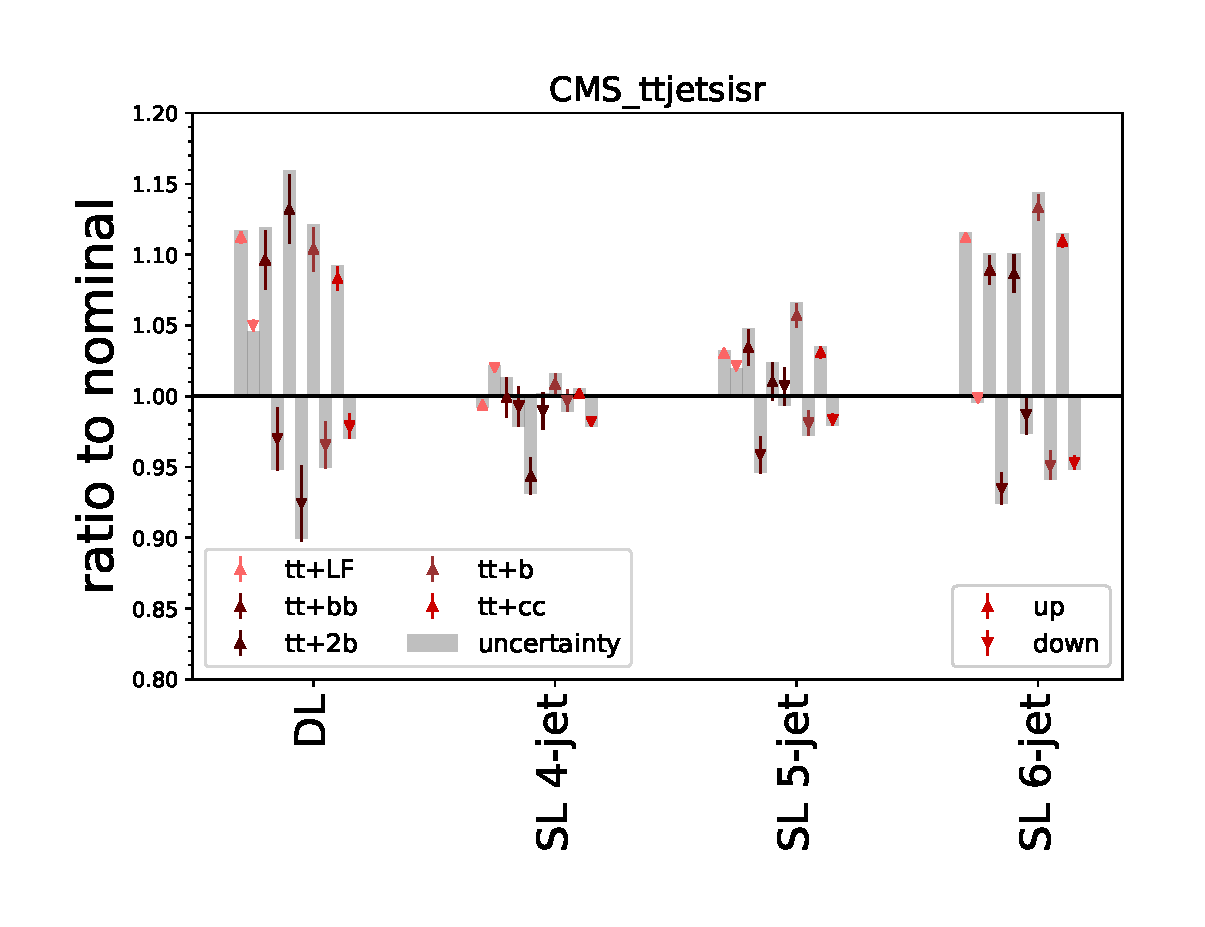
\includegraphics[width=1.0\textwidth]{figures/tth/CMS_ttjetsisr.pdf}
\caption[The \ttbar+jets ISR modelling uncertainties]{The \ttbar+jets ISR modelling uncertainties in terms of a scale factor that depends on jet multiplicity. We extract this scale factor by comparing the yield predicted by the MC simulation with varied parameter values to the nominal, adding the statistical uncertainty on this prediction. Generally, these scale factors are symmetric around the nominal and change the yield by $<15\%$, with the most significant effects on the \ttlf~process.}
\label{fig:tth_ttjets_modelling}
\end{centering}
\end{figure}

\begin{figure}
\begin{centering}
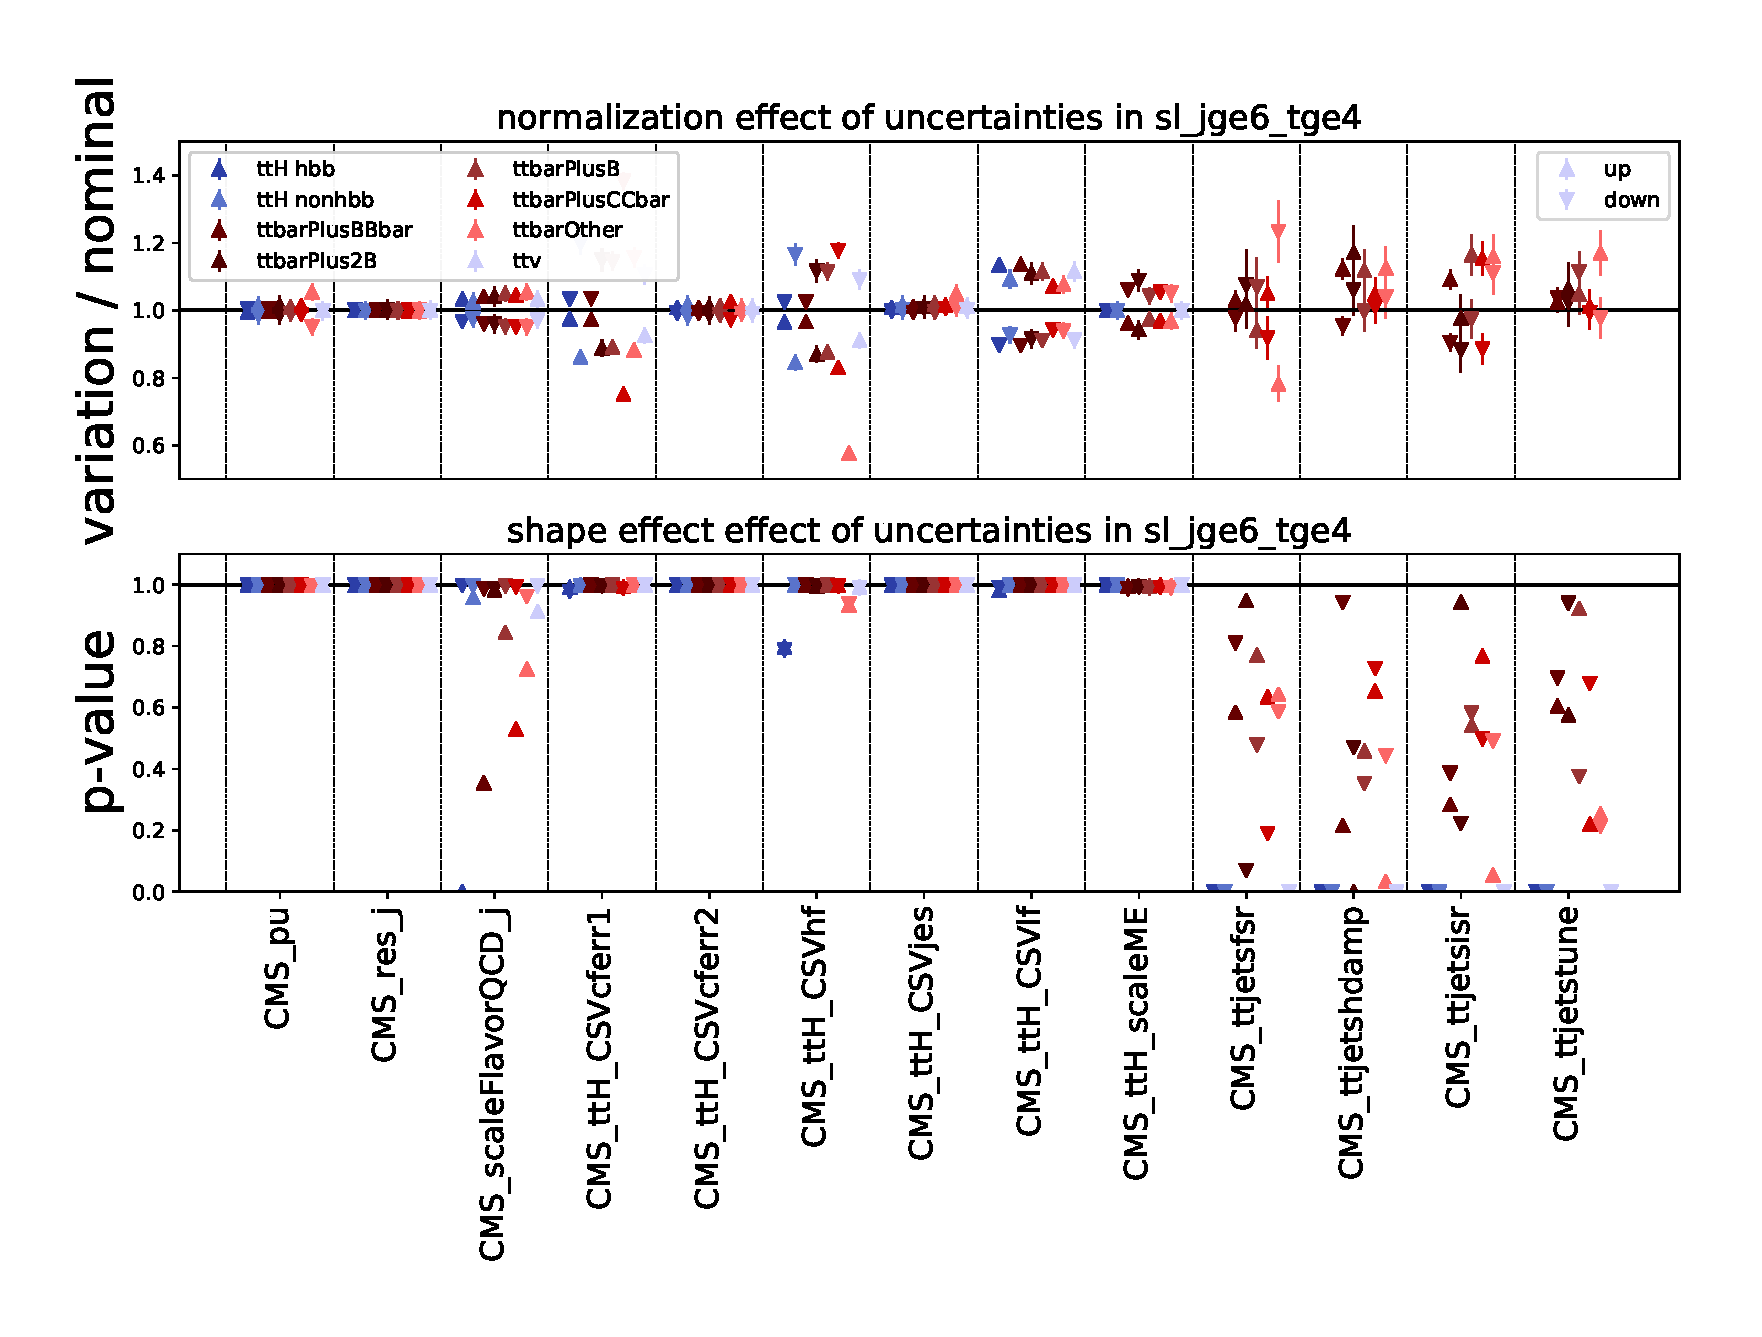
\includegraphics[width=1.0\textwidth]{figures/tth/uncs_sl_jge6_tge4.pdf}
\caption[The normalisation and shape effect of uncertainties]{The normalisation and shape effect of the most important shape-changing uncertainties. In the top figure, we show the effect on the normalisation in terms of the ratio between the varied and nominal predictions. In the figure in the bottom, we show the estimated effect on the shape of the template by computing the p-value from the $\chi^2$ test between the two histograms. We see that generally the effect of shape variations is symmetric, with a yield change that is under 20\%. Most shape changes are consistent with no change, apart from the JES flavour uncertainty and the b~tagging heavy flavour uncertainty. The ISR, FSR, $h_{\mathrm{damp}}$ and MC tune uncertainties do not have enough simulation statistics to determine the presence of shape changes. These uncertainties are verified using MC simulation in the semileptonic category with at least six jets, out of which four must be b~tagged.}
\label{fig:tth_uncertainties_effect}
\end{centering}
\end{figure}

\subsection{Control regions}
We validate the MC simulation in the inclusive semileptonic and dileptonic control regions with at least four jets, out of which at least two must be b~tagged by comparing the simulated distributions of jet and lepton kinematic variables to data. The distributions in the semileptonic control region can be seen in~\cref{fig:tth_sl_control} and for the dileptonic in~\cref{fig:tth_dl_control}. In general, we see that both the inclusive yields and differential distributions for the kinematic variables are well-described within the systematic uncertainties. We observe a residual mismodeling in the jet multiplicity distribution, which we attribute to uncertainties in the modelling of the parton shower and the \ttbar+jets MC tuning.

\begin{figure}
\begin{centering}
\subfloat{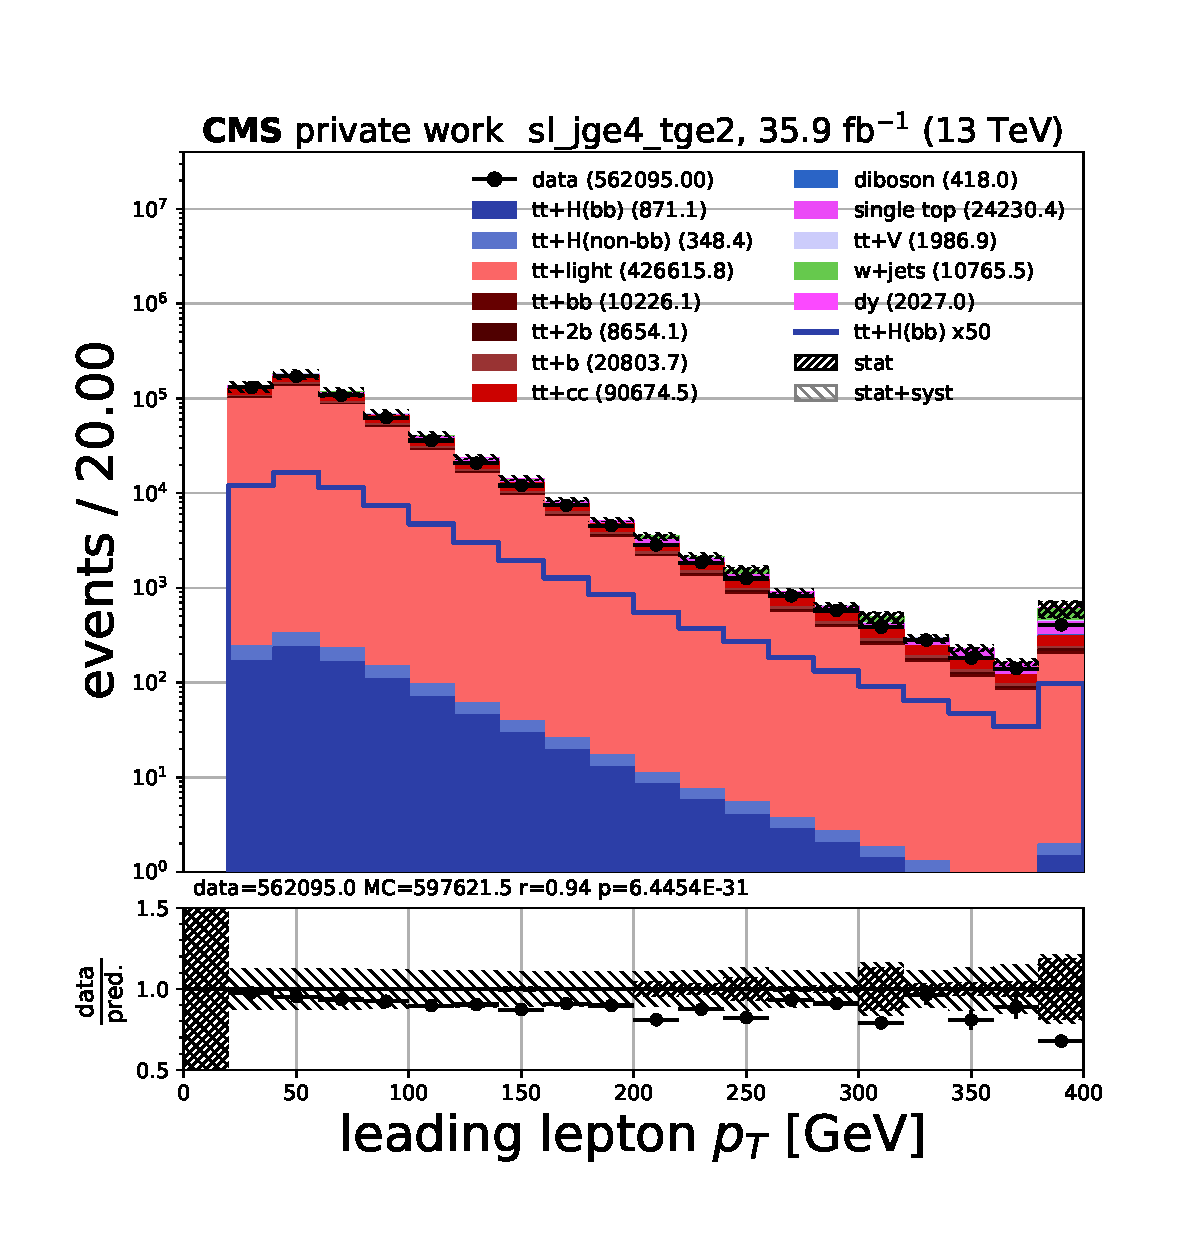
\includegraphics[width=0.45\textwidth]{figures/tth/sl_jge4_tge2/leps_0_pt.pdf}}
\subfloat{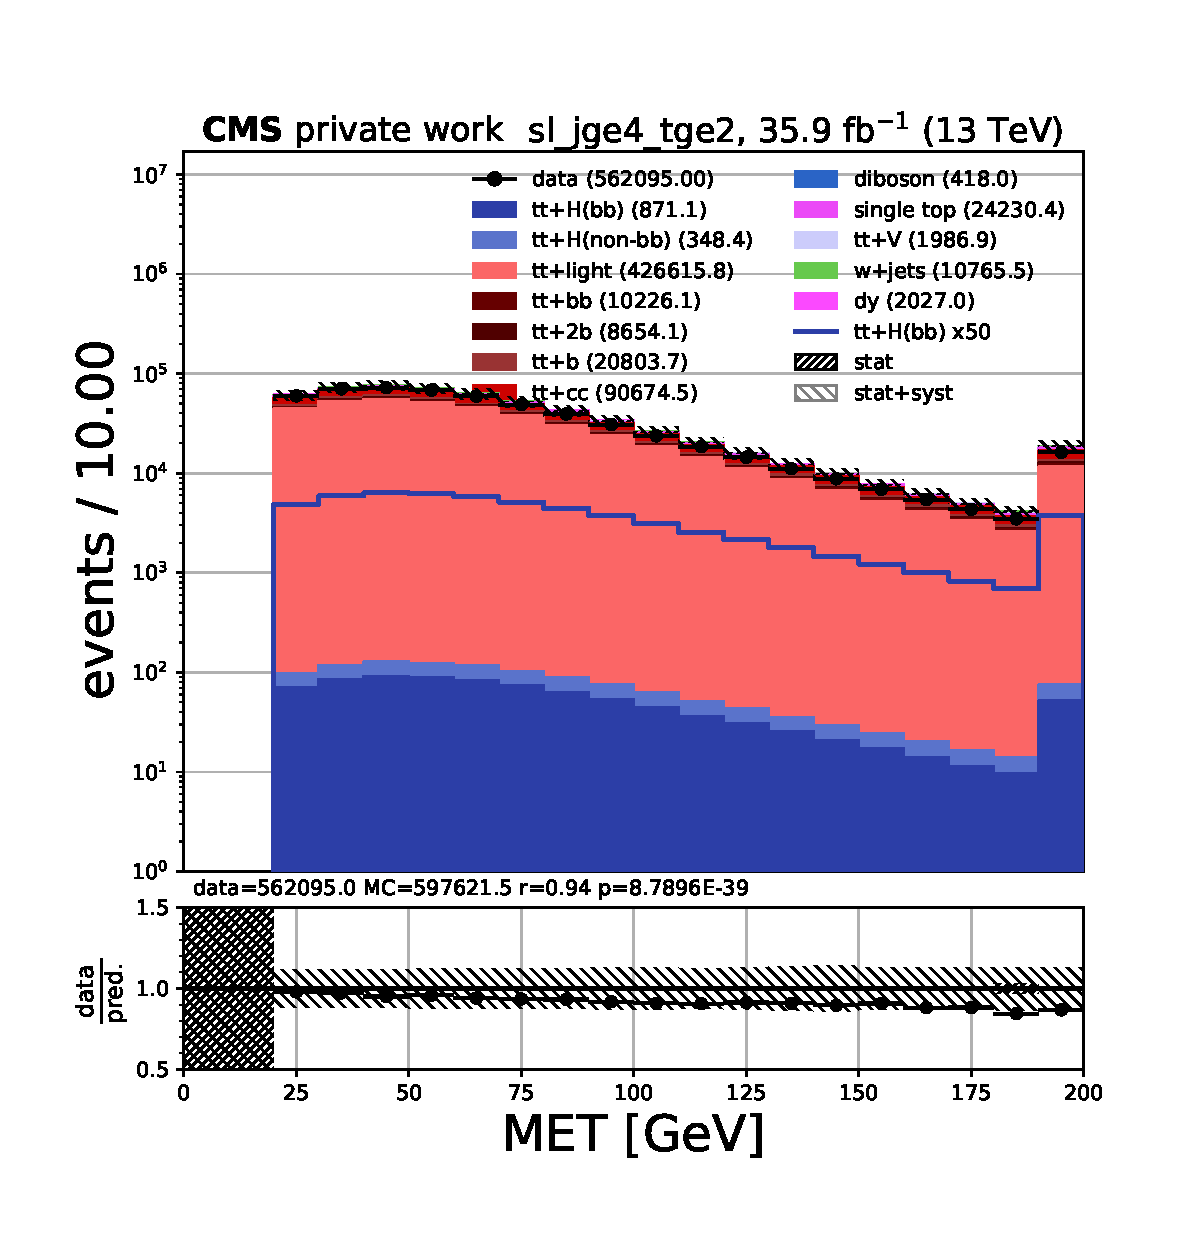
\includegraphics[width=0.45\textwidth]{figures/tth/sl_jge4_tge2/met_pt.pdf}} \\

\subfloat{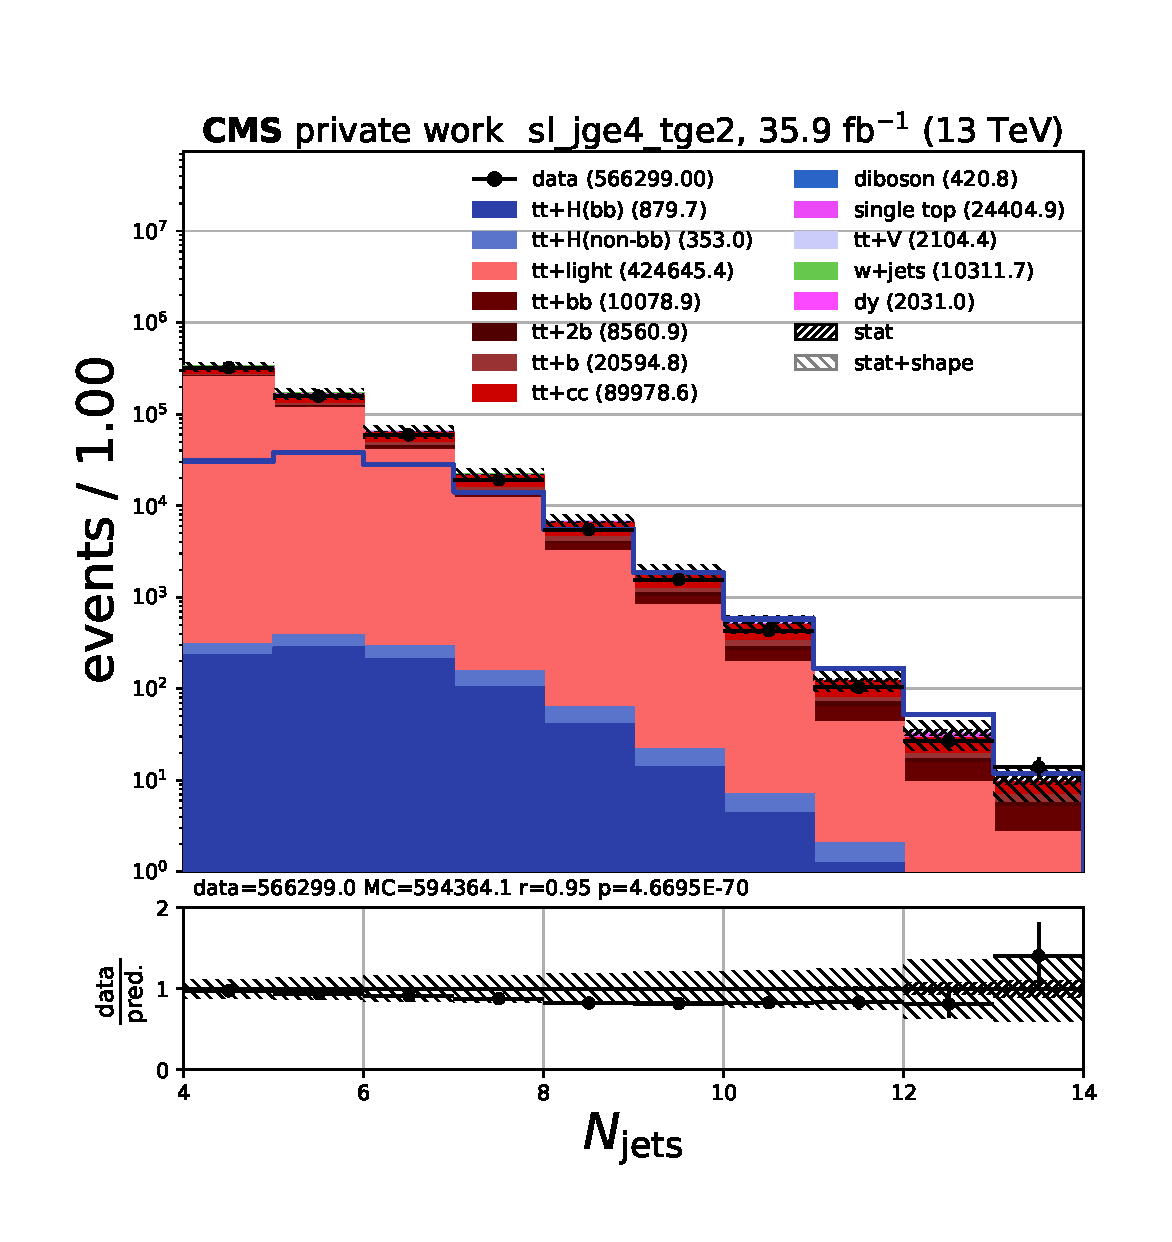
\includegraphics[width=0.45\textwidth]{figures/tth/sl_jge4_tge2/numJets.pdf}}
\subfloat{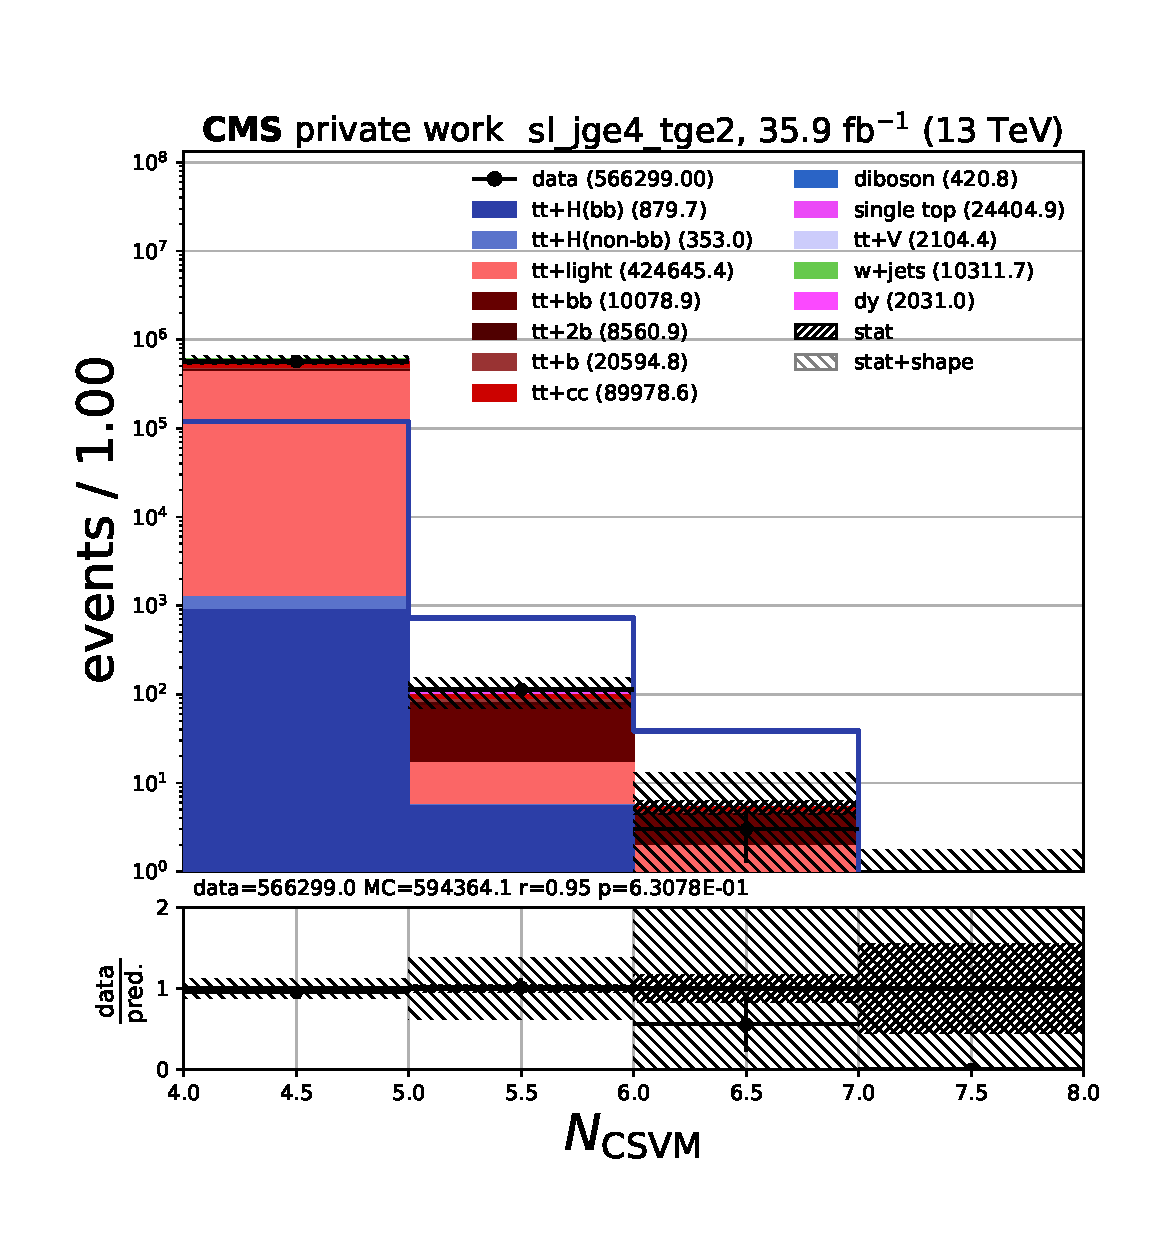
\includegraphics[width=0.45\textwidth]{figures/tth/sl_jge4_tge2/nBCSVM.pdf}} \\

\subfloat{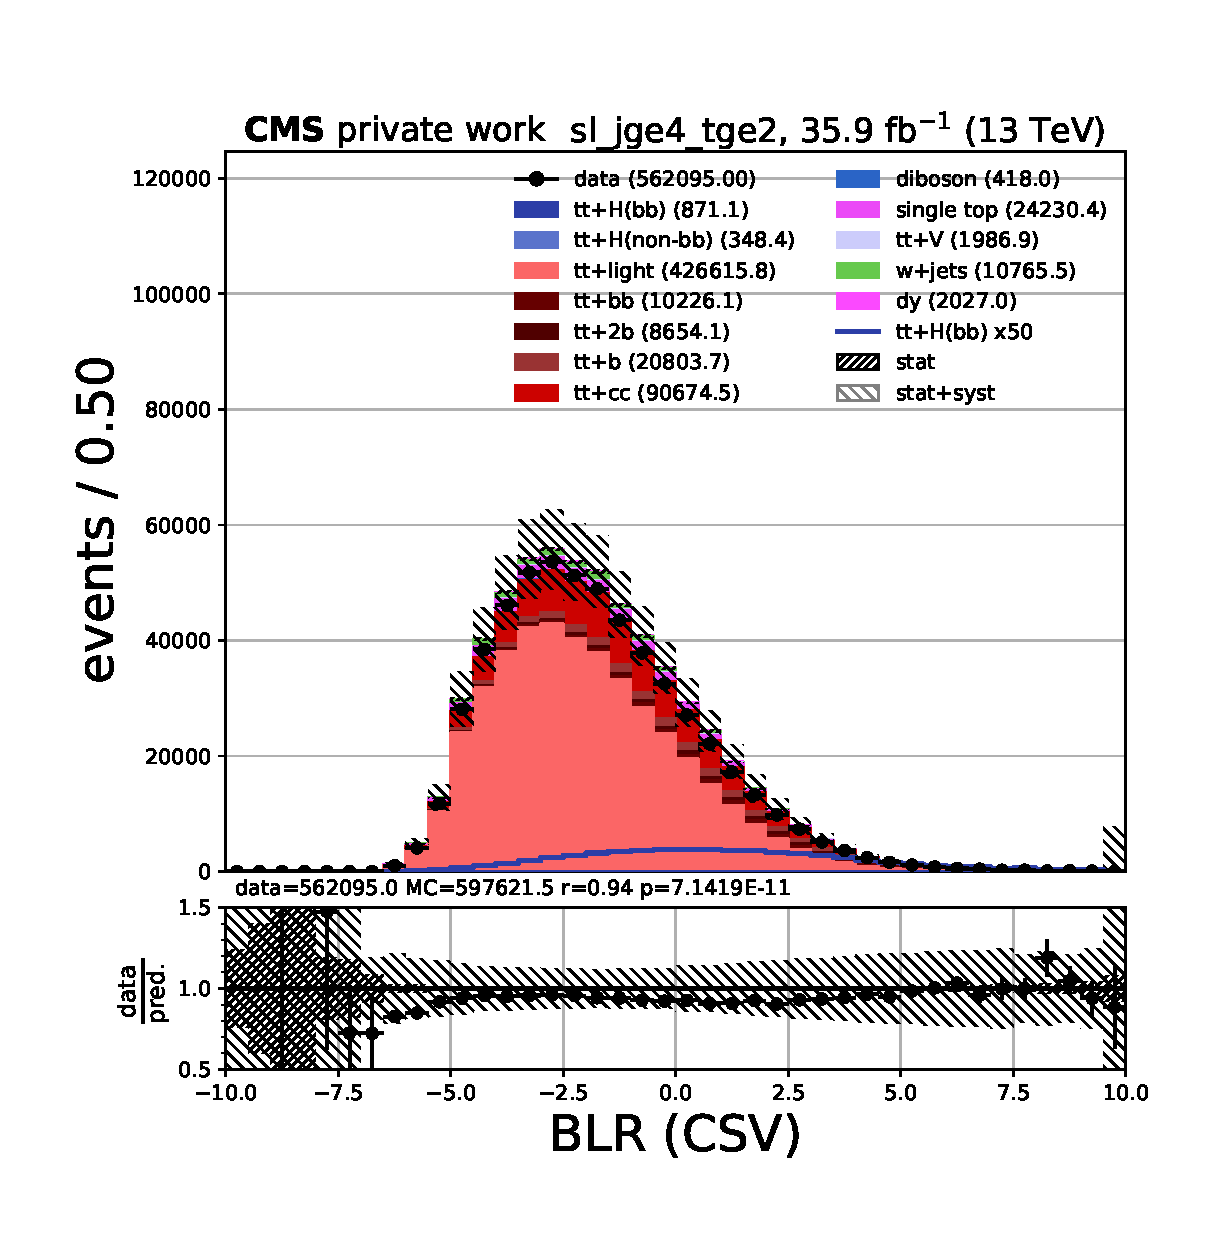
\includegraphics[width=0.45\textwidth]{figures/tth/sl_jge4_tge2/btag_LR_4b_2b_btagCSV_logit.pdf}}
\subfloat{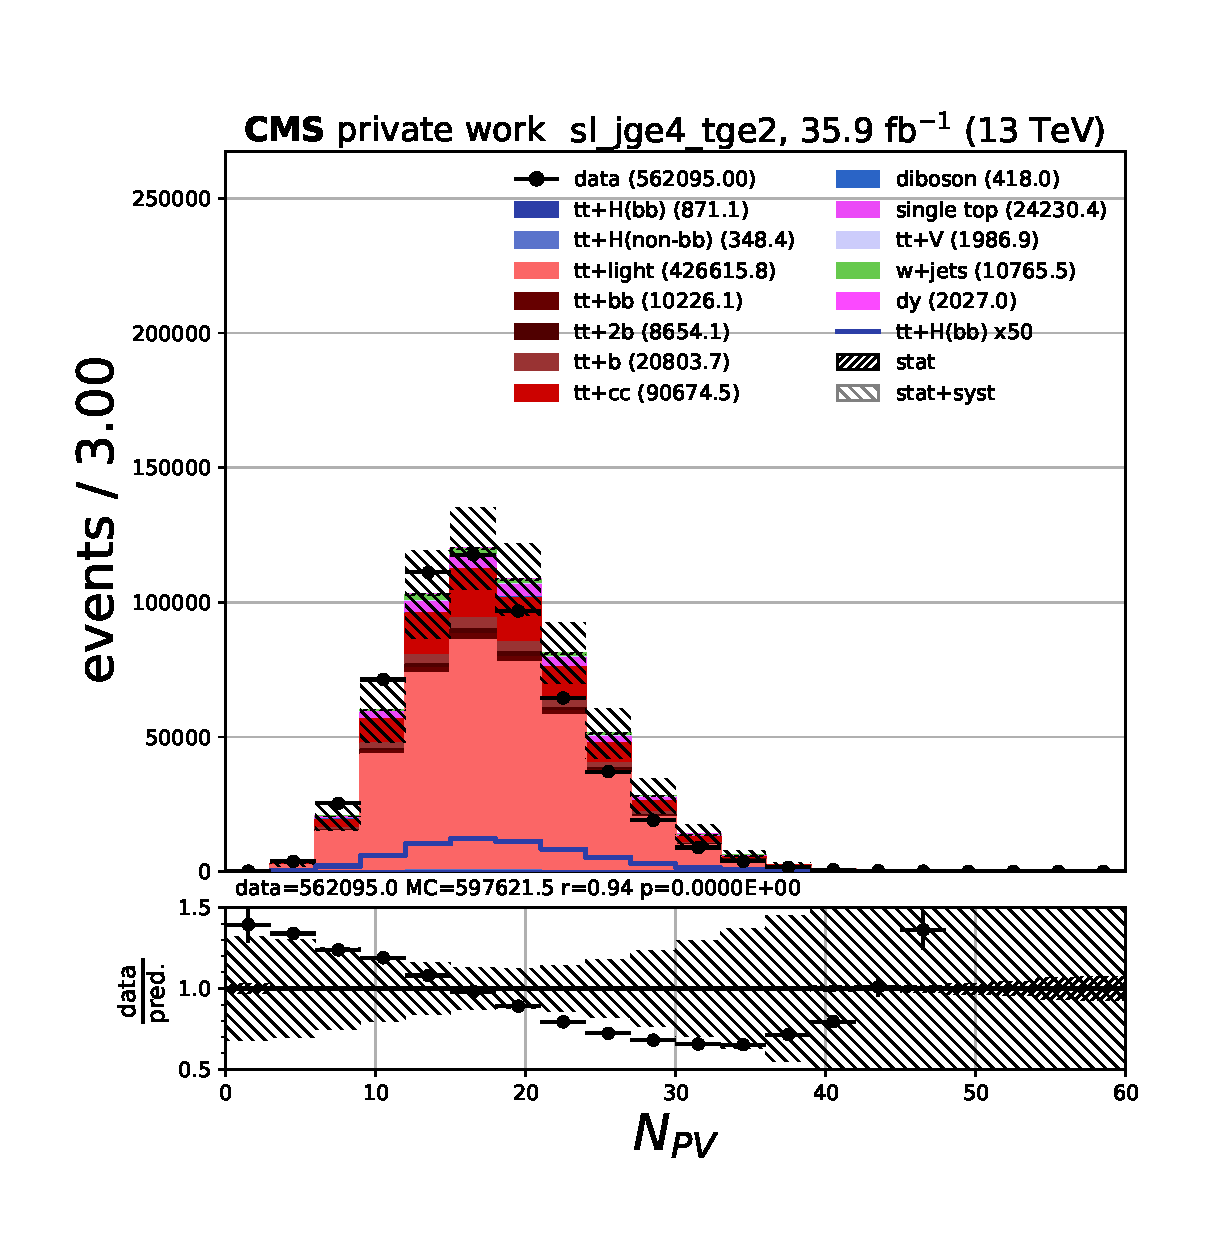
\includegraphics[width=0.45\textwidth]{figures/tth/sl_jge4_tge2/nPVs.pdf}} \\
\caption[The modelling of the kinematic distributions in the semileptonic control region]{The modelling of the most important analysis variables in the semileptonic control region with at least four jets, out of which two must be b~tagged.}
\label{fig:tth_sl_control}
\end{centering}
\end{figure}

\begin{figure}
\begin{centering}
\subfloat{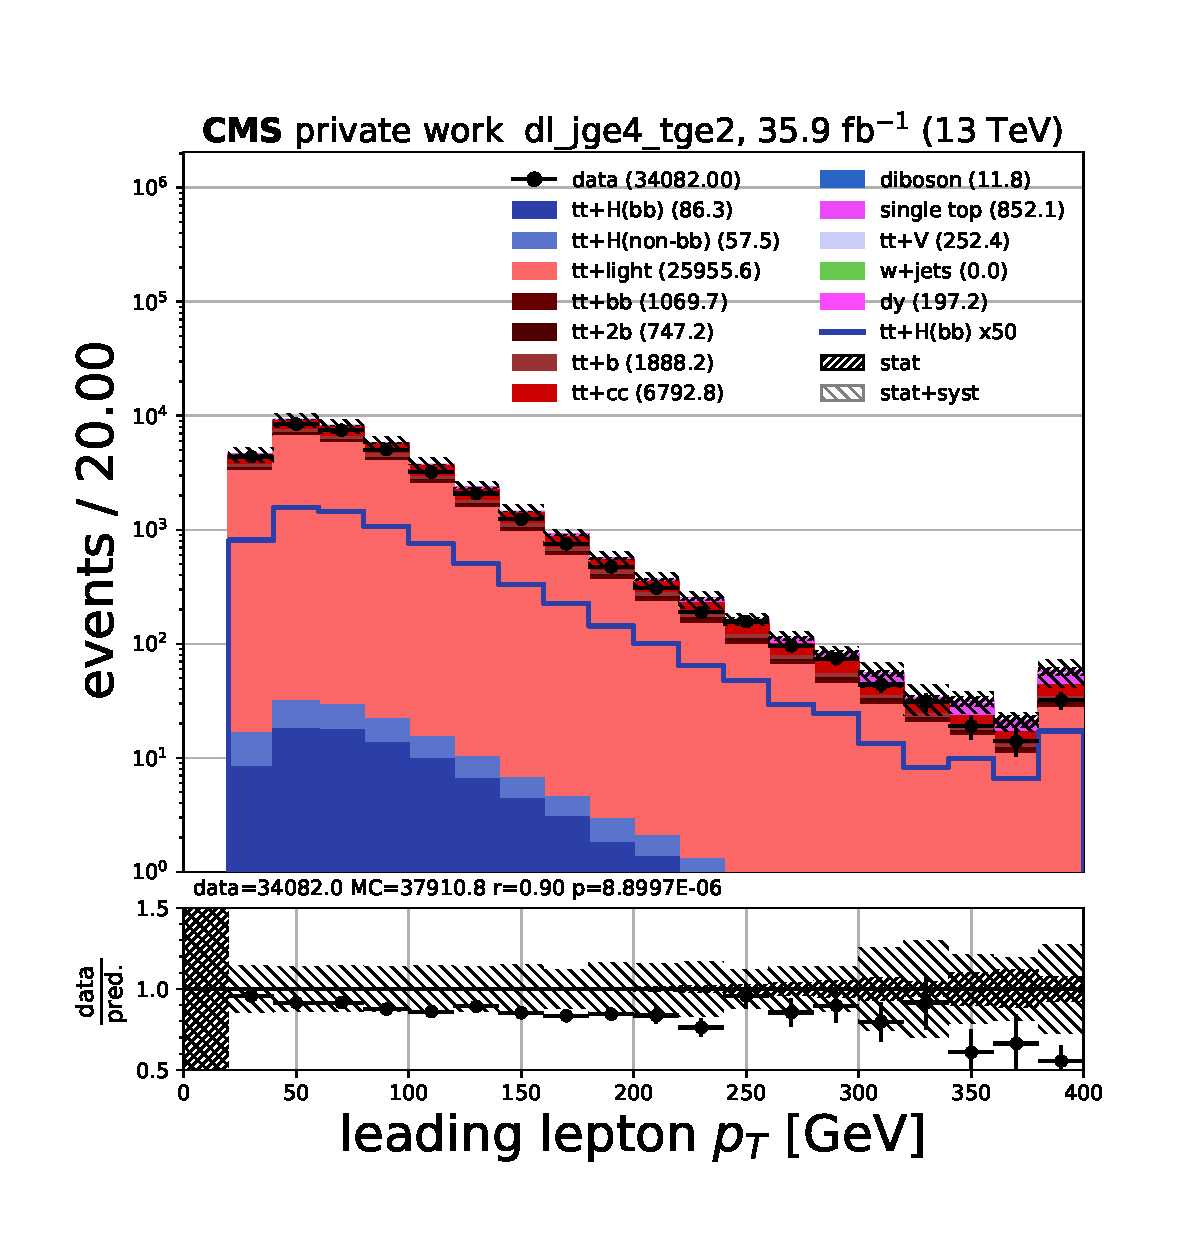
\includegraphics[width=0.45\textwidth]{figures/tth/dl_jge4_tge2/leps_0_pt.pdf}}
\subfloat{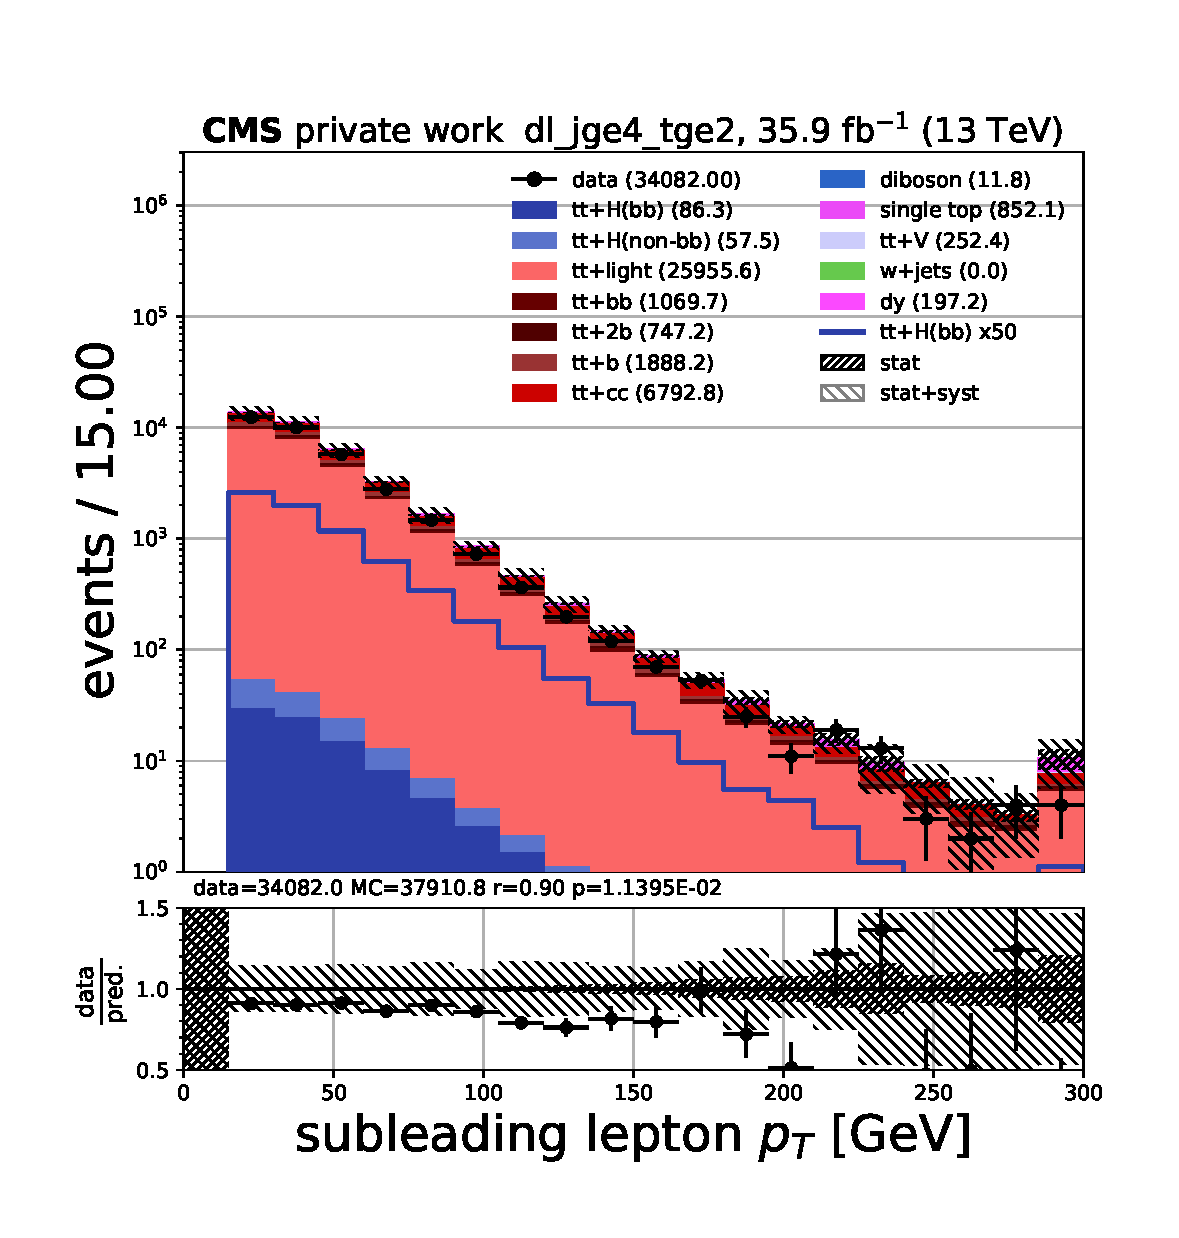
\includegraphics[width=0.45\textwidth]{figures/tth/dl_jge4_tge2/leps_1_pt.pdf}} \\

\subfloat{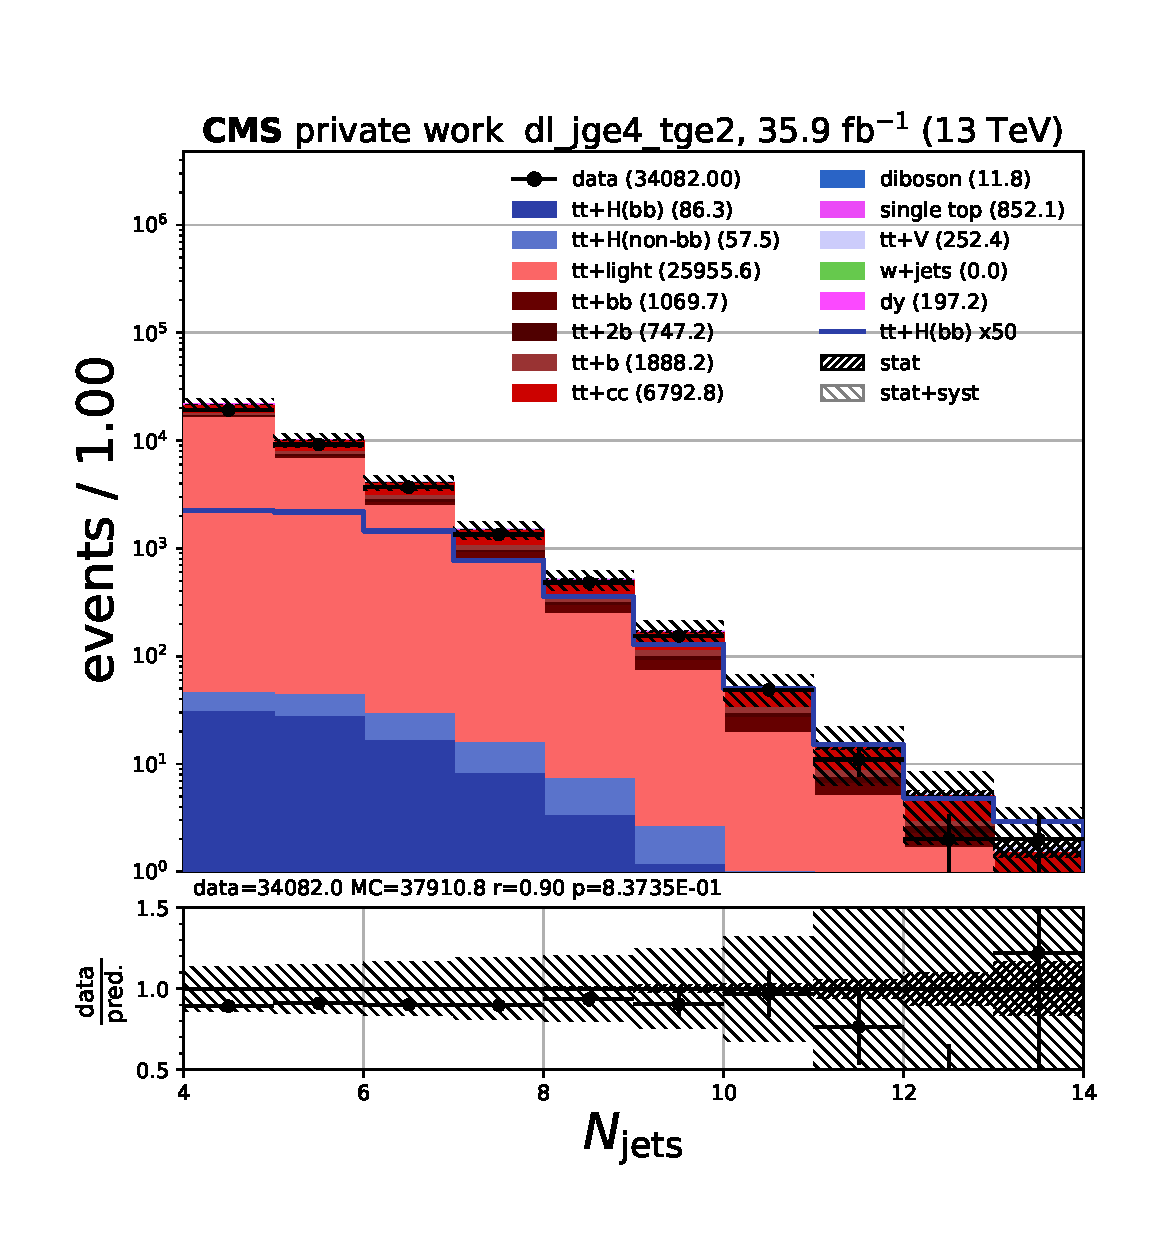
\includegraphics[width=0.45\textwidth]{figures/tth/dl_jge4_tge2/numJets.pdf}}
\subfloat{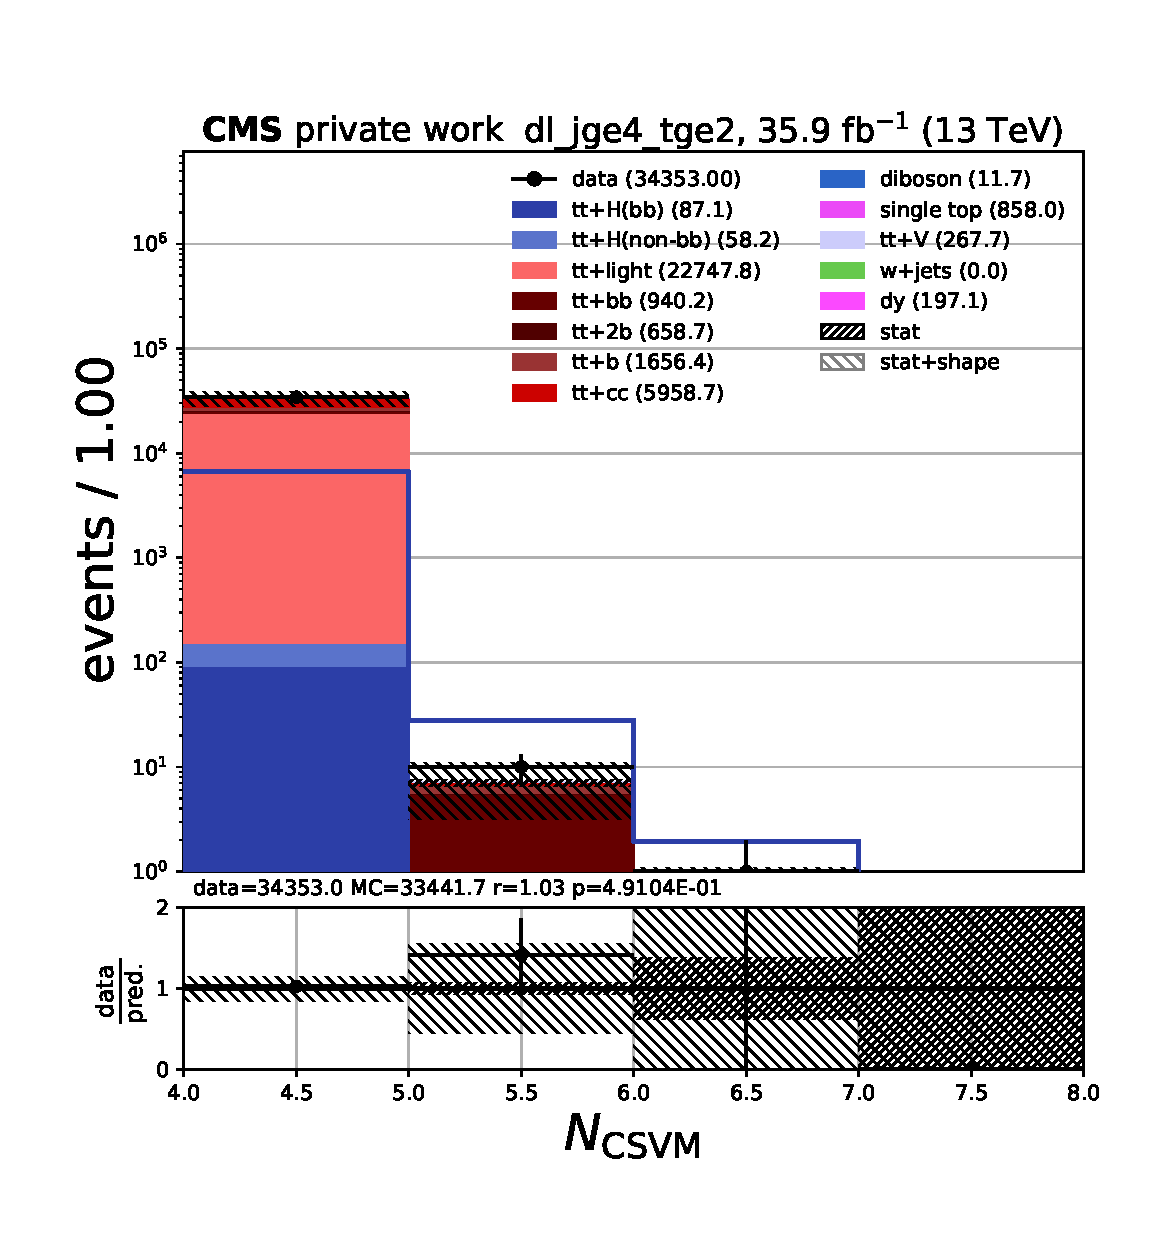
\includegraphics[width=0.45\textwidth]{figures/tth/dl_jge4_tge2/nBCSVM.pdf}} \\

\subfloat{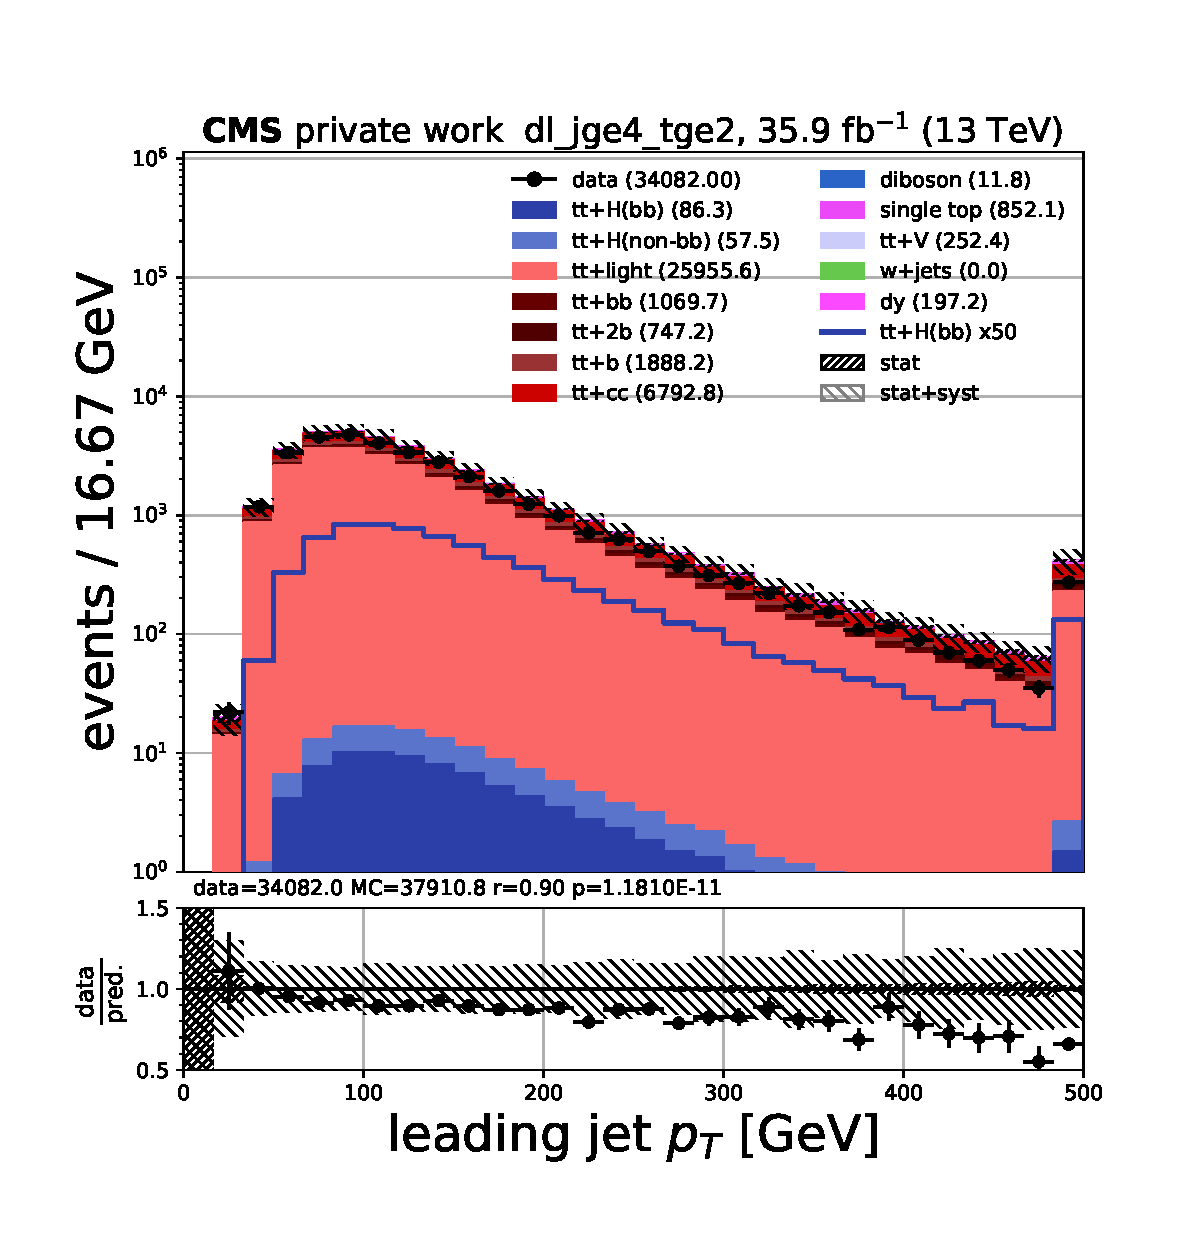
\includegraphics[width=0.45\textwidth]{figures/tth/dl_jge4_tge2/jetsByPt_0_pt.pdf}}
\subfloat{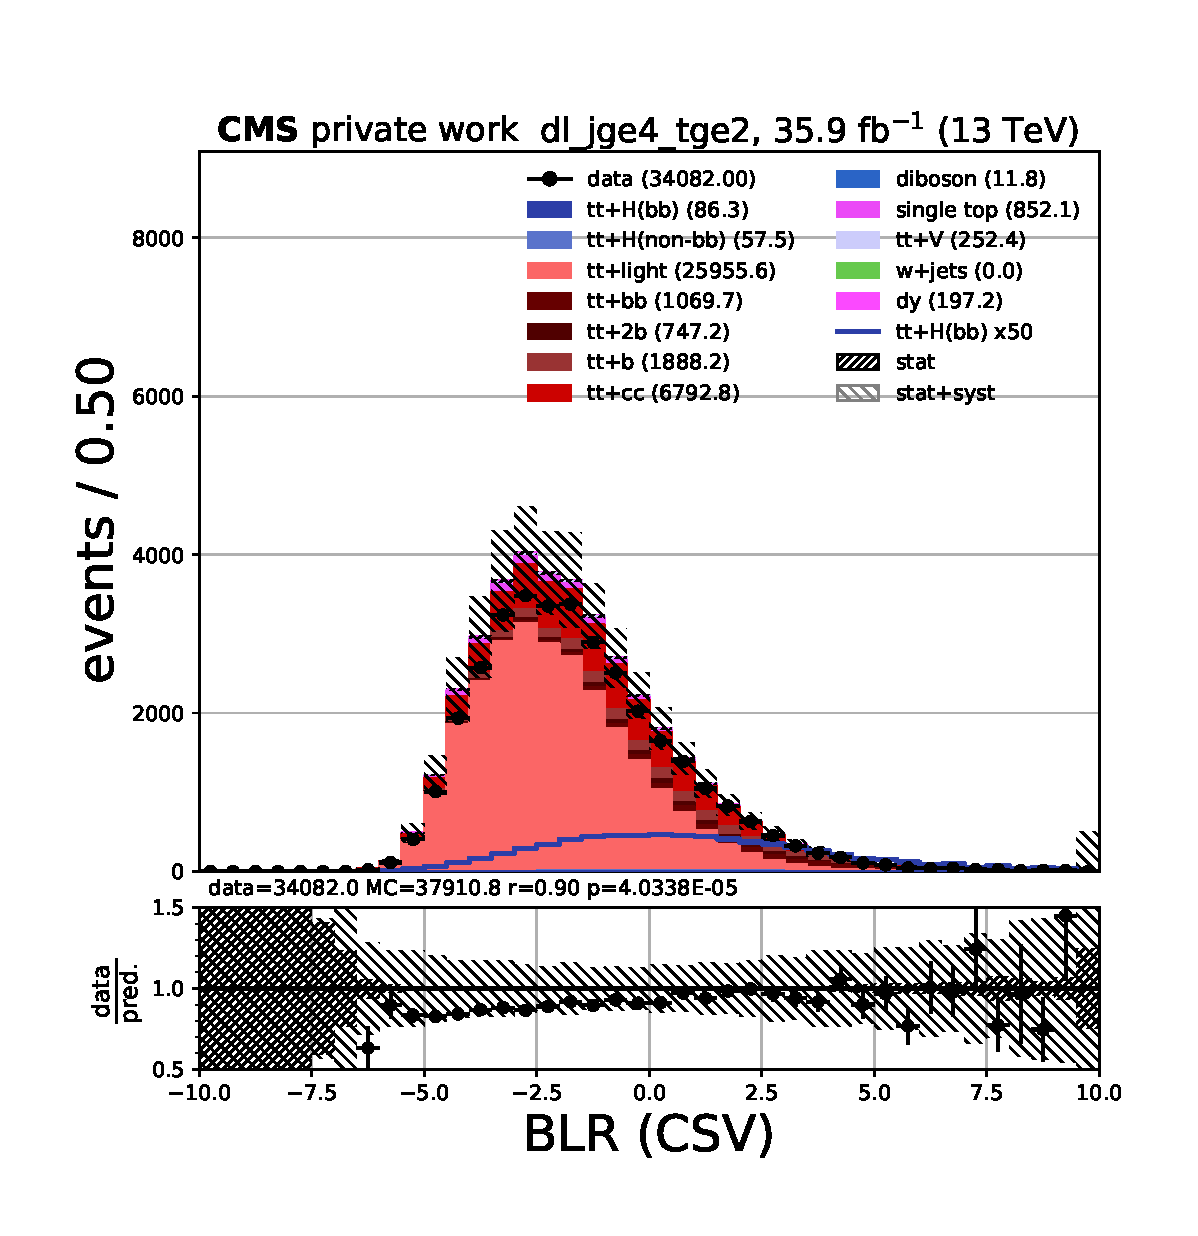
\includegraphics[width=0.45\textwidth]{figures/tth/dl_jge4_tge2/btag_LR_4b_2b_btagCSV_logit.pdf}} \\

\caption[The modelling of the kinematic distributions in the dileptonic control region]{The modelling of the most important analysis variables in the dileptonic control region with at least four jets, out of which two must be b~tagged.}
\label{fig:tth_dl_control}
\end{centering}
\end{figure}


\subsection{Statistical method}
\label{sec:statistical_method}
In order to interpret the data, we use the same statistical framework as has been used for other Higgs boson searches in the CMS collaboration~\cite{Chatrchyan:2012xdj,Chatrchyan:2012tx,ATLAS:2011tau}. We wish to measure the signal strength modifier~$\mu = \sigma_{\ttH}/\sigma_{\ttH}^{\mathrm{SM}}$~and in the absence of an observed signal, exclude~$\mu \ge \mu^{CL}$~at a certain confidence level. The null hypothesis ($H_0$) is therefore the presence of a signal with a given~$\mu$, whereas the alternative hypothesis is no signal ($H_1, \mu = 0~$). Based on the data, we seek to exclude the null hypothesis above a certain~$\mu$.

The predicted distributions for both signal (denoted as~$s$) and background (denoted as~$b$) are subject to uncertainties introduced in~\cref{sec:systematic_unc} such that the expectations are functions of the nuisance parameters~$\theta$ through~$s(\theta)$~and~$b(\theta)$. The uncertainties are assumed to be either fully correlated or uncorrelated, as is more appropriate and conservative, which allows the likelihood function to be written in a factorised form.

To determine confidence intervals on the Higgs boson production cross section and thus quantify the presence or absence of a signal, we use the~$CL_s$~method~\cite{Junk:1999kv,Read:2002}, which defines the likelihood function~$\mathcal{L}(\mathrm{data} | \mu, \theta)$~as

\begin{align}
\label{eq:likelihood}
\mathcal{L}(\mathrm{data} | \mu, \theta) =&  \mathrm{Poisson}[\mathrm{data} | \mu \cdot s(\theta) + b(\theta)] \cdot p(\tilde{\theta} | \theta)\\
=& \prod_{i\in \mathrm{bins}} \frac{(\mu s_i + b_i)^{n_i}}{n_i!} \exp{[-(\mu s_i + b_i)]} \cdot p(\tilde{\theta} | \theta).
\end{align}
We have used Poisson probabilities to model the observation of~$n_i$~events in the bin~$i$~of a discretised distribution, given an expectation~$\mu s_i + b_i$. The distribution~$p(\tilde{\theta} | \theta)$~encodes the prior knowledge on the nuisance parameters, which have default values~$\tilde{\theta}$. This likelihood function can be computed both with observed data and with ``pseudo-data'', which is constructed from simulation under a specific hypothesis.

We use the test statistic~$\tilde{q}_\mu$, based on the profile likelihood ratio~\cite{Cowan:2010js}, to assess the compatibility of the data with either the \textit{background-only} or \textit{signal+background} hypotheses:

\begin{equation}
\tilde{q}_\mu = -2 \ln{\frac{\mathcal{L}(\mathrm{data} | \mu, \hat{\theta}_\mu)}{\mathcal{L}(\mathrm{data} | \hat{\mu}, \hat{\theta})}} = -2 \ln{\lambda(\mu)},\ 0 \le \hat{\mu} \le \mu.
\end{equation}
This test statistic is constructed such that it considers only models with~$\mu \ge 0$, furthermore it is constrained to be one-sided by~$\hat{\mu} \le \mu$~such that data with~$\hat{\mu} > \mu$~are not used as part of the rejection region for the test on the upper limit of~$\mu$.

Here~$\hat{\theta}_\mu$~is the conditional maximum likelihood estimator of~$\theta$~given a fixed value~$\mu$, whereas $\hat{\mu}$~and $\hat{\theta}$ refer to the overall maximum likelihood estimators of both quantities. For a given signal strength modifier~$\mu$~that we test, we first find the observed value of~$\tilde{q}_\mu^{\mathrm{obs}}$~and the nuisance parameters~$\hat{\theta}_0$~(background hypothesis) and~$\hat{\theta}_\mu$~(signal hypothesis). Then, in order to compute the~$\mathrm{CL}_s(\mu)$, we compute the p-values of the signal and background hypotheses using

\begin{equation}
p_{\mu} = \int_{\tilde{q}_{\mu}{\mathrm{obs}}}^\infty f(\tilde{q}_{\mu} | \mu, \hat{\theta}_{\mu})\ \mathrm{d}\tilde{q}_\mu
\end{equation}
and

\begin{equation}
1 - p_b = \int_{\tilde{q}_{\mu}^{\mathrm{obs}}}^\infty f(\tilde{q}_{\mu} | 0, \hat{\theta}_0)\ \mathrm{d}\tilde{q}_{\mu}.
\end{equation}

The p-values are the probabilities of observing results as extreme or more given the underlying hypothesis and are derived from the probability densities of~$\tilde{q}_{\mu}$~under a given hypothesis:~$f(\tilde{q}_\mu | \mu, \hat{\theta}_\mu^{\mathrm{obs}})$. We find the 95\% confidence level on the upper limit of~$\mu$~by adjusting~$\mu$~until

\begin{equation}
\mathrm{CL}_s(\mu) = \frac{p_\mu}{1 - p_b} < 0.05.
\end{equation}
Equivalently, if~$\mathrm{CL}_s < \alpha$~at~a given $\mu$, then the Higgs boson is excluded at a production rate of~$\mu$~or higher with a confidence level~$1 - \alpha$.

In order to compute the upper limit on~$\mu$~given the observed data, we need the PDFs $f(\tilde{q}_\mu | \mu, \hat{\theta}_\mu^{\mathrm{obs}})$, which can be derived using a Monte Carlo method by generating pseudo-data assuming the given signal strength~$\mu$~and fitting the observed data to evaluate the test statistic. As the MC procedure for generating the PDFs can be very time consuming, we use an approximate asymptotic distribution~\cite{Cowan:2010js} for the PDF~$\tilde{q}_\mu$, which results from the Wald approximation for the profile likelihood~\cite{wald1943tests}:

\begin{equation}
-2 \ln{\lambda(\mu)} = \frac{(\mu - \hat{\mu})^2}{\sigma^2}+ \mathcal{O}(1/\sqrt{N})
\end{equation}
where~$\sigma$~is the standard deviation of~$\hat{\mu}$~derived from the full covariance matrix of the likelihood function.

Using the asymptotic distribution for~$f(\tilde{q}_\mu | \mu, \hat{\theta}_\mu^{\mathrm{obs}})$, we find the upper limit for~$\mu$~at a confidence level of~$1 - \alpha$~to be

\begin{equation}
\mu = \hat{\mu} + \sigma \Phi^{-1}(1 - \alpha)
\end{equation}
where~$\Phi^{-1}$~is the inverse of the cumulative distribution of the Gaussian PDF. The standard deviation of~$\mu$~can be computed from the likelihood function~\cref{eq:likelihood} using the so-called Asimov data set, where the SM prediction is used for~$s_i$~and~$b_i$.

We will also quote the expected sensitivity of the measurement, which is derived from simulation, assuming~$\mu = 1$~and computing the median expected upper limit on~$\mu$~using the asymptotic formulae. 

\subsubsection{Uncertainties in the statistical model}

Our prior knowledge of the systematic uncertainties is encoded in~$p(\tilde{\theta} | \theta)$, where the values of the nuisance parameters~$\theta$~are determined by minimising the likelihood function in a frequentist sense. We use~$\tilde{\theta}$~to represent our best pre-fit estimate of the nuisance parameters, which can be
\begin{itemize}
\item Gaussian, used for shape variations,
\item log-normal used for nuisance parameters for which negative values are unphysical,
\item flat, in case we cannot assign a prior uncertainty.
\end{itemize}
In order to account for limited MC statistics, we create nuisance parameters for each process and bin in the template distributions, corresponding to the Poisson uncertainties from the limited number of simulation events.
%We use the Barlow-Beeston method in the fit to account for limited number of simulation events. In this method, the number of predicted events for a background component in a binned distribution is added as a nuisance parameter in the likelihood and minimized with the initial values arising from the observed Poisson counts using Newton's method~\cite{Barlow:1993dm}. 

\subsection{Analysis of the statistical model}
\label{sec:model_analysis}
In this section, we will study the expected sensitivity as predicted by the statistical model. We have used pseudo-data constructed from MC simulation with the SM expectation ($\mu=1$) and a no-signal model ($\mu=0$) as representative datasets. The nuisance parameters are set to the priors, with central values at 0 and relative variances at 1, compared to the pre-fit expectation. This is the Asimov principle, where an ensemble of datasets is replaced by a single representative dataset~\cite{Cowan:2010js}.

First, in order to validate the fit model, we study the effect of systematic uncertainties in the form of pulls and constraints on the nuisance parameters after the fit to pseudo-data derived from MC. We compute the pulls and constraints, defined as the central value and the width of the distribution $(\hat{\theta} - \theta_0) / \Delta\theta$ with respect to the pre-fit values $\theta_0$, with the uncertainty $\Delta\theta$ determined around the minimum of the likelihood function. By fitting the signal+background and background-only models on the background-only dataset, we verify that both models result in equivalent constraints and no pulls, as can be seen in~\cref{fig:tth_sldl_pulls}.

We further determine that in the fit to the $\mu=1$ Asimov dataset, some of the nuisances in the background-only model will be shifted with respect to their pre-fit values to compensate the mismatch between the background-only model and the signal+background dataset. In particular, we observe a negative pull in the heavy flavour modelling of the b~discriminator and positive pulls for the \ttbb~normalisation and \ttbar+jets ISR modelling, showing that these nuisance parameters are (anti)-correlated to the signal strength parameter $\mu$. When fitting the signal+background model on the $\mu=1$ dataset, we observe constraints at the level of $\mathrm{Var}[(\hat{\theta} - \theta_0)/\Delta \theta] \simeq 0.5$ for these nuisances, from which we surmise that the model has sensitivity for these nuisance parameters with respect to the prior uncertainties. This is expected, as the prior uncertainties on some of the nuisance parameters are assumed to be quite large in the absence of a detailed description by MC. We can see that the correlation between the best-fit values of the signal strength $\mu$ and the nuisance parameters is significant, by determining the best-fit values as a function of the \ttbb\xspace background normalisation nuisance parameter $\theta_{\ttbb}$, as shown in~\cref{fig:tth_nuis_scan}.

\begin{figure}
\setlength{\floatsep}{1pt}
\begin{centering}
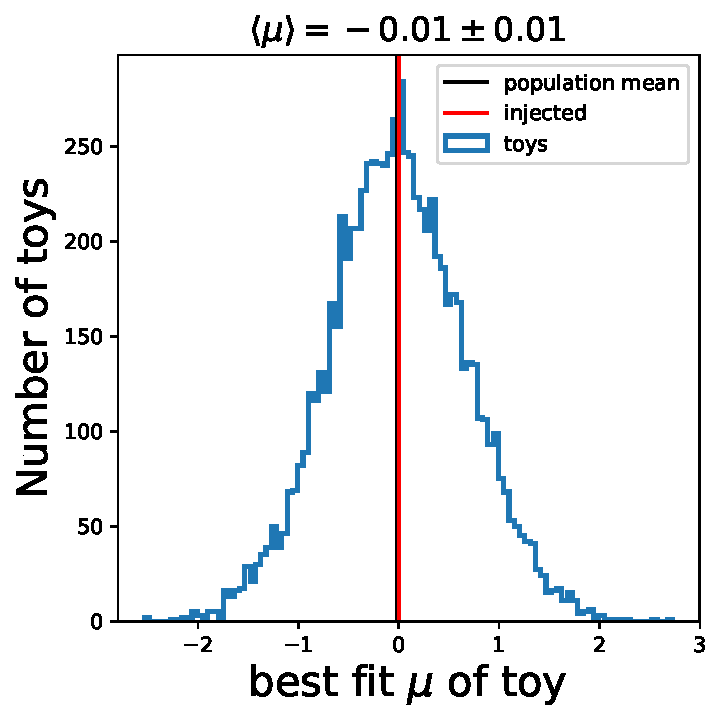
\includegraphics[width=0.30\textwidth]{figures/tth/mu_sig_group_sldl_0_0.pdf}
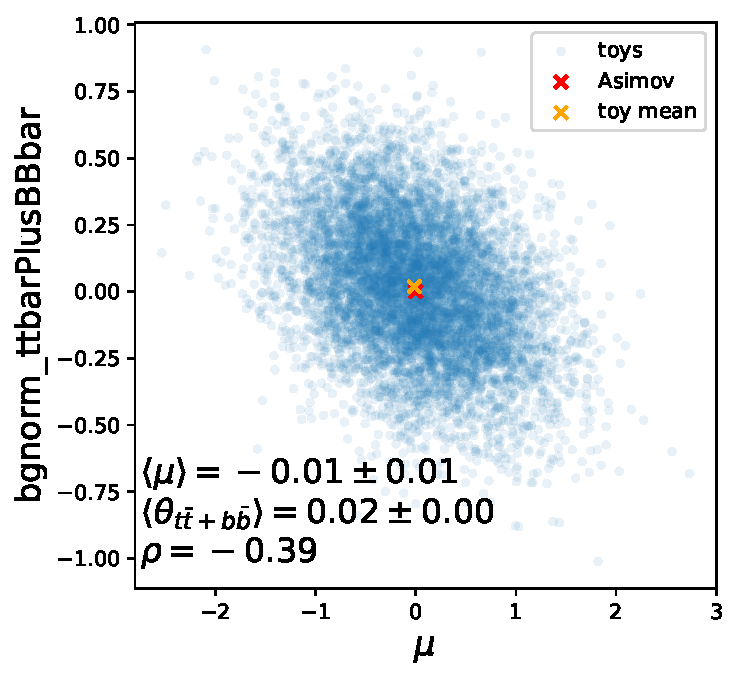
\includegraphics[width=0.30\textwidth]{figures/tth/mu_bgnorm_ttbarPlusBBbar_sig_group_sldl_0_0.pdf}\\
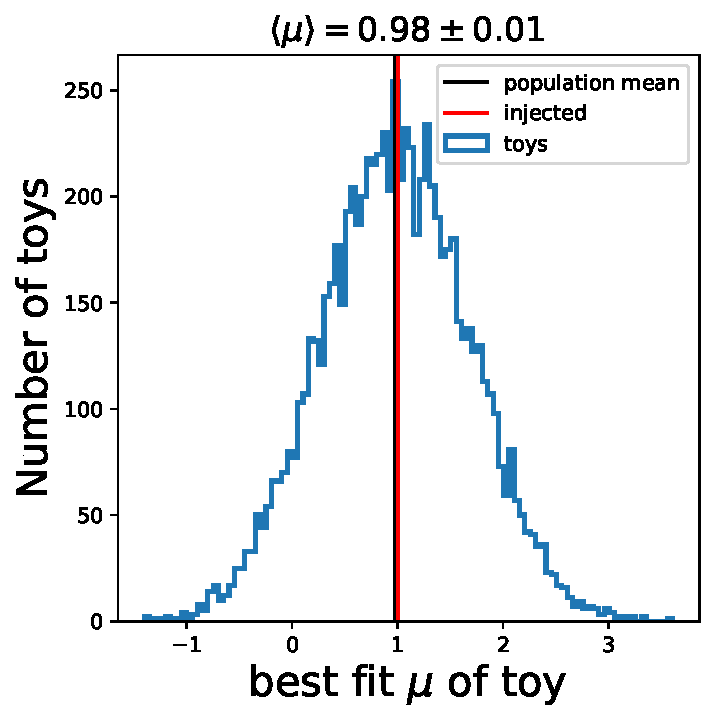
\includegraphics[width=0.30\textwidth]{figures/tth/mu_sig_group_sldl_1_0.pdf}
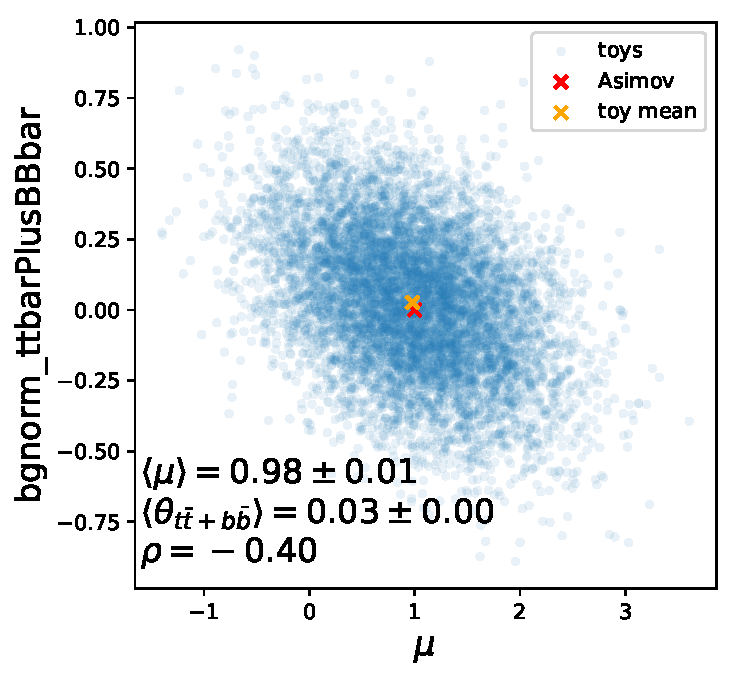
\includegraphics[width=0.30\textwidth]{figures/tth/mu_bgnorm_ttbarPlusBBbar_sig_group_sldl_1_0.pdf}\\
\caption[Fit model validation on toy experiments]{On the left, the distribution of the best-fit values $\hat{\mu}$ for toy experiments sampled from the $\mu=0$ dataset (top row) and from the $\mu=1$ dataset (bottom row). On the right, we show $\hat{\mu}$ with respect to $\hat{\theta}_{\ttbb}$. We see that the expected anti-correlation between these parameters is reproduced by the model.}
\label{fig:tth_toy_studies}
\end{centering}
\end{figure}

Furthermore, in order to test deviations from the Wald approximation, we generate toy datasets from the MC expectation by sampling the nuisance parameters from their prior distributions and perform individual fits for each such sample. We see in~\cref{fig:tth_toy_studies} that the mean of the best-fit signal strength parameter $\langle \hat{\mu} \rangle$ reproduces the prior value to within $\Delta\mu \simeq 0.01$ and thus the approximation generally holds for our model. 

\begin{figure}
\setlength{\floatsep}{1pt}
\begin{centering}
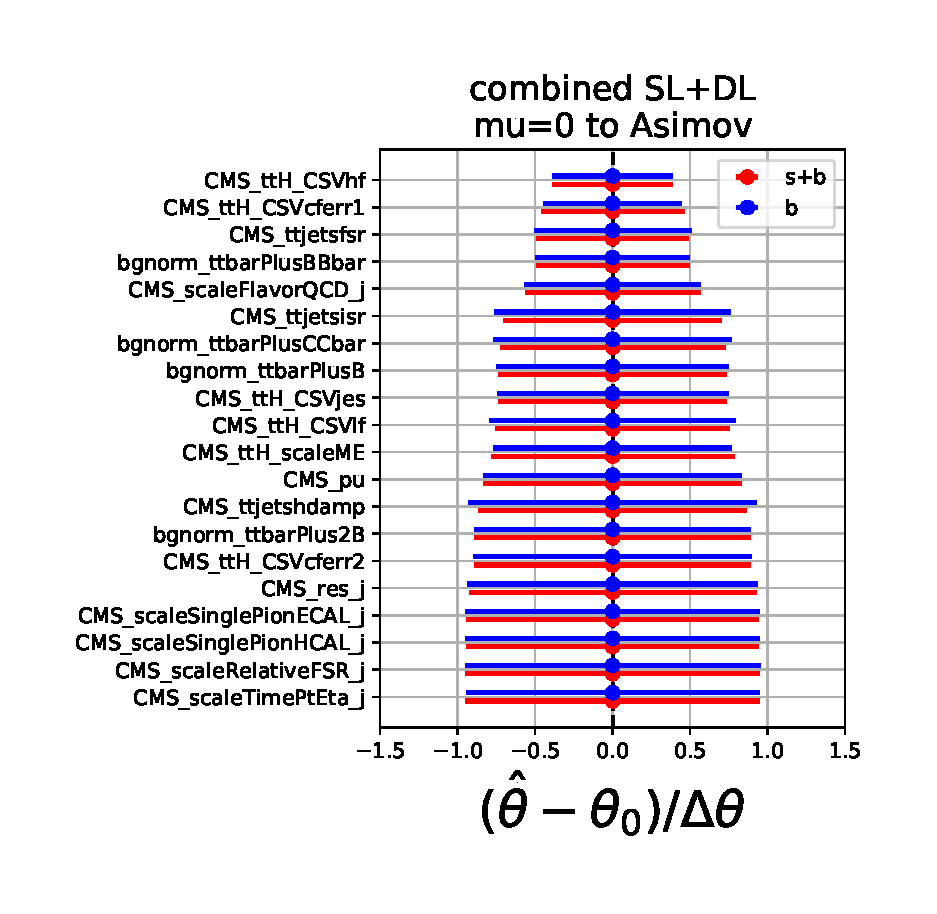
\includegraphics[width=0.45\textwidth]{figures/tth/pulls_group_sldl_sig0_r0_20_asimov.pdf}
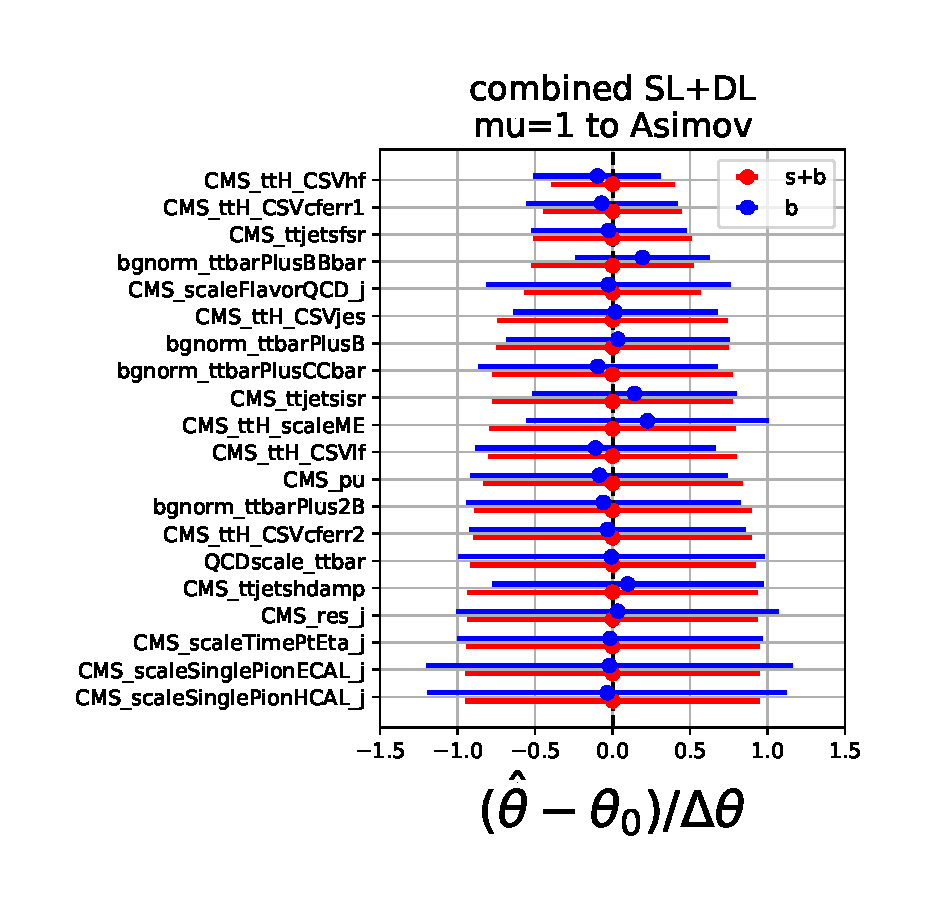
\includegraphics[width=0.45\textwidth]{figures/tth/pulls_group_sldl_sig1_r0_20_asimov.pdf}\\
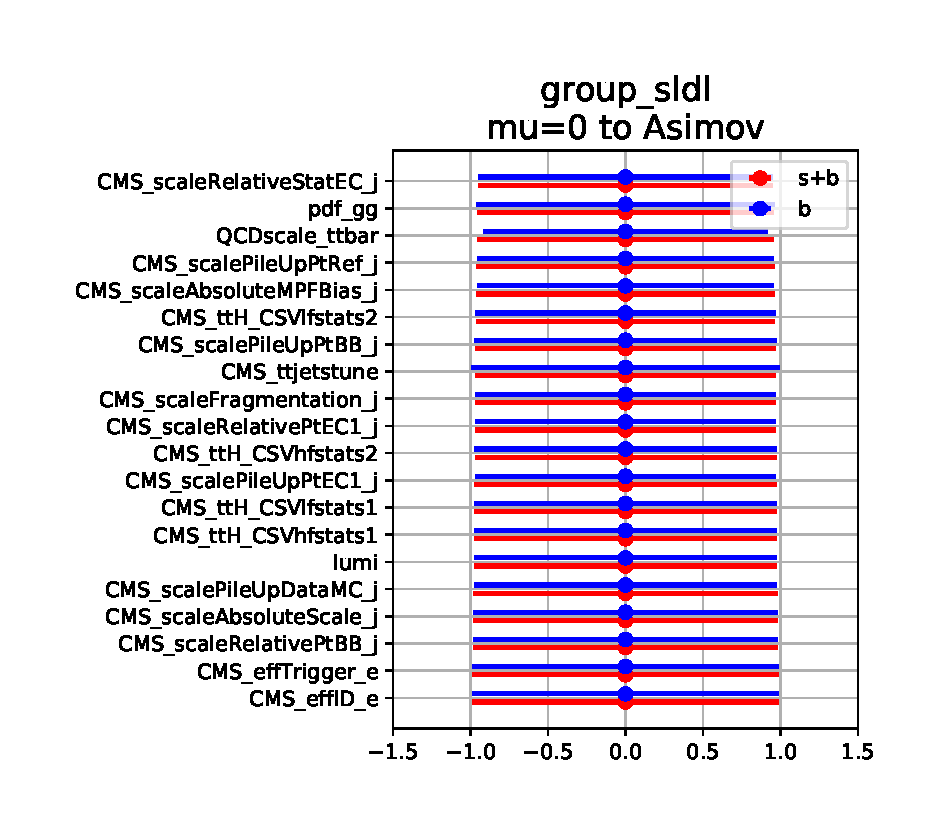
\includegraphics[width=0.45\textwidth]{figures/tth/pulls_group_sldl_sig0_r20_40_asimov.pdf}
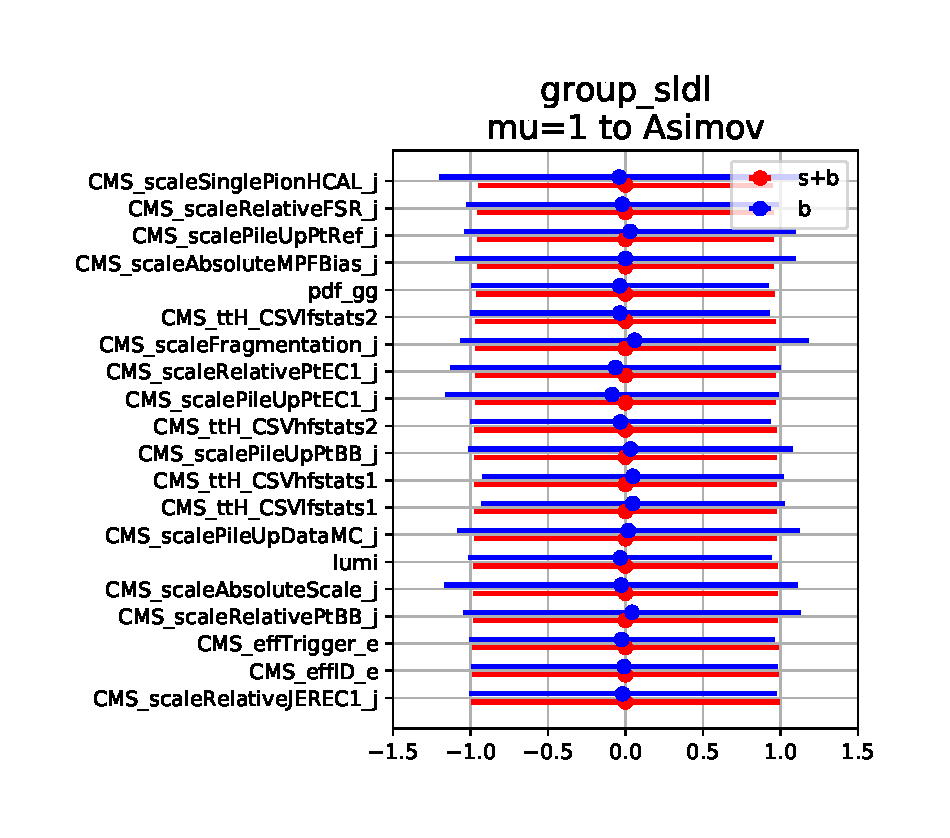
\includegraphics[width=0.45\textwidth]{figures/tth/pulls_group_sldl_sig1_r20_40_asimov.pdf}\\
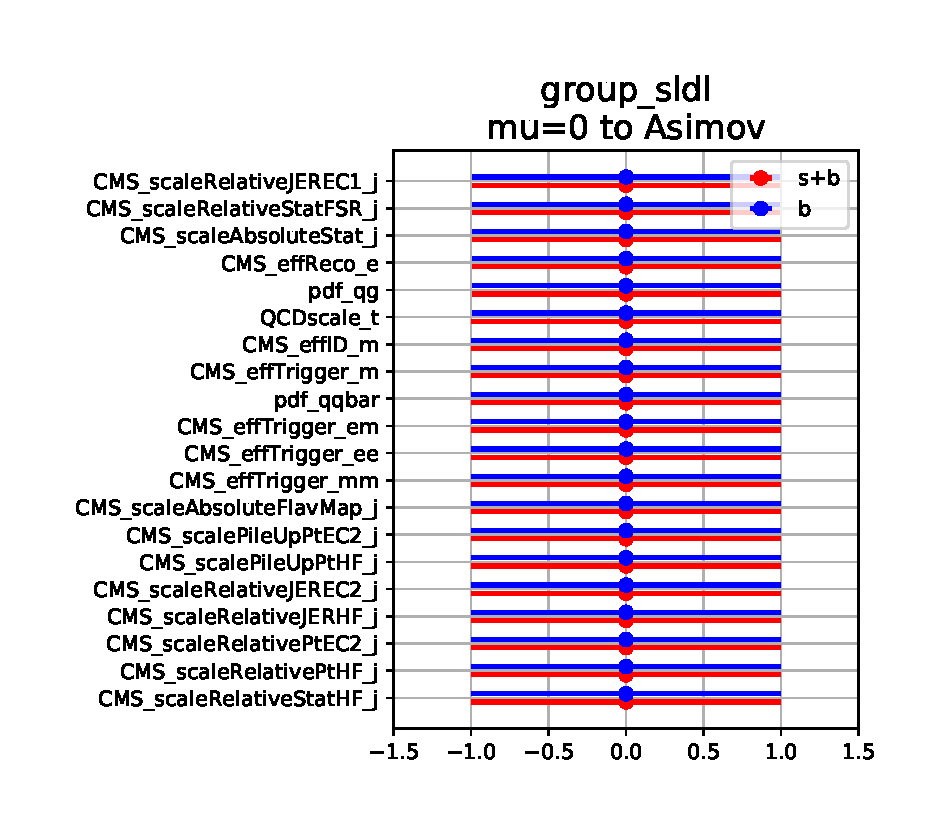
\includegraphics[width=0.45\textwidth]{figures/tth/pulls_group_sldl_sig0_r40_60_asimov.pdf}
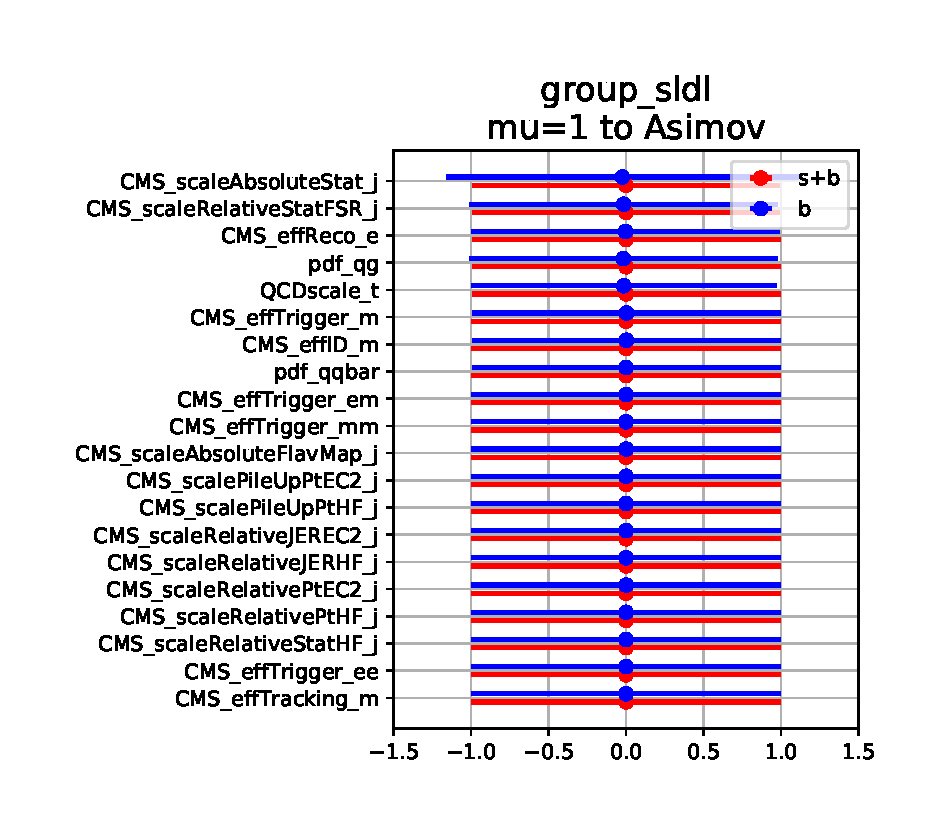
\includegraphics[width=0.45\textwidth]{figures/tth/pulls_group_sldl_sig1_r40_60_asimov.pdf}
\caption[The pulls and constraints of the combined fit model with the Asimov datasets]{The pulls and constraints on the nuisance parameters of the background-only model (blue) and the signal+background model (red) on the $\mu=0$ Asimov dataset (left) and the $\mu=1$ Asimov dataset (right). The nuisances are ordered by ascending constraint size (width of the pull distribution), shown as the error bar around the pull $\hat{\theta} / \theta$.  We only show the first 60 nuisance parameters that experience the most significant constraints, out of the full list of $\mathcal{O}(600)$. For the $\mu=1$ Asimov dataset, we observe the strongest constraints at around $\hat{\sigma_{\theta}} \simeq 0.5$ for the CSV b~discriminator heavy flavour modelling (\texttt{CMS\_ttH\_CSVhf}), the \ttbb~normalisation (\texttt{bgnorm\_ttbarPlusBBbar}), the \ttbar+jets FSR modelling (\texttt{CMS\_ttjetsfsr}) and the b~discriminator charm flavour modelling (\texttt{CMS\_ttH\_CSVcferr1}).}
\label{fig:tth_sldl_pulls}
\end{centering}
\end{figure}


\begin{figure}
\begin{centering}
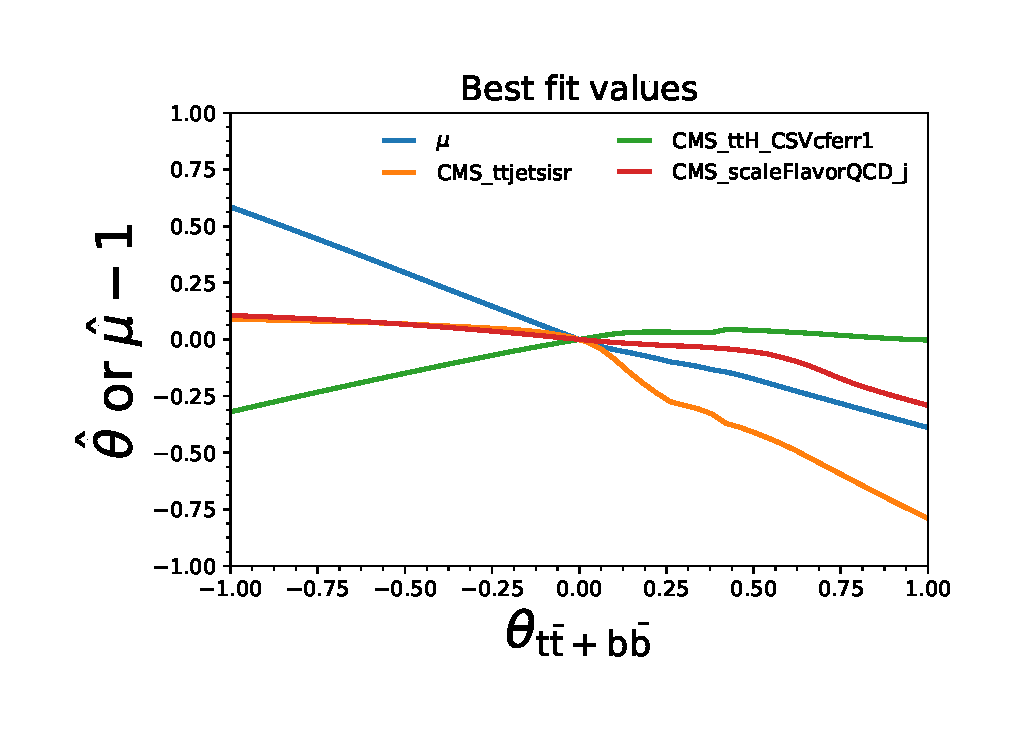
\includegraphics[width = 0.7\textwidth]{figures/tth/nuis_scan.pdf}
\caption[The best-fit estimations of nuisance parameters as a function of the $\theta_{\ttbb}$ nuisance parameter]{The best-fit estimations of the signal strength parameter $\mu$ and other significant nuisance parameters as a function of the \ttbb\xspace normalisation uncertainty ($\theta_{\ttbb}$) nuisance parameter. We see that the best-fit value of the signal strength parameter is anti-correlated to $\theta_{\ttbb}$, and other nuisance parameters have a non-trivial dependence on the chosen value of $\theta_{\ttbb}$.}
\label{fig:tth_nuis_scan}
\end{centering}
\end{figure}

\section{Results}
\label{sec:tth_results}
After having validated the statistical model on simulation using the Asimov dataset, we carry out the analysis on the observed data by using the real dataset instead of the Asimov dataset from the MC expectation. A combined fit across all categories is used to extract the signal strength parameter $\mu$. We show the pre-fit and post-fit distributions in the final categories in~\cref{fig:tth_postfit1,fig:tth_postfit2,fig:tth_postfit3,fig:tth_postfit4}. The uncertainty is reduced by the fit and the post-fit description of the data is generally good, with p-values for the goodness of fit test at the level of $p=0.8-0.99$ for the individual categories. We observe a downward fluctuation in the MEM distribution in the DL $\geq4$ jets, $\geq4$ tags category, which is compatible with the MC expectation within one standard deviation. The post-fit p-value in this category is $p\simeq 0.87$.

\begin{figure}
\begin{centering}
\setlength{\floatsep}{5pt plus 1.0pt minus 2.0pt}
\subfloat{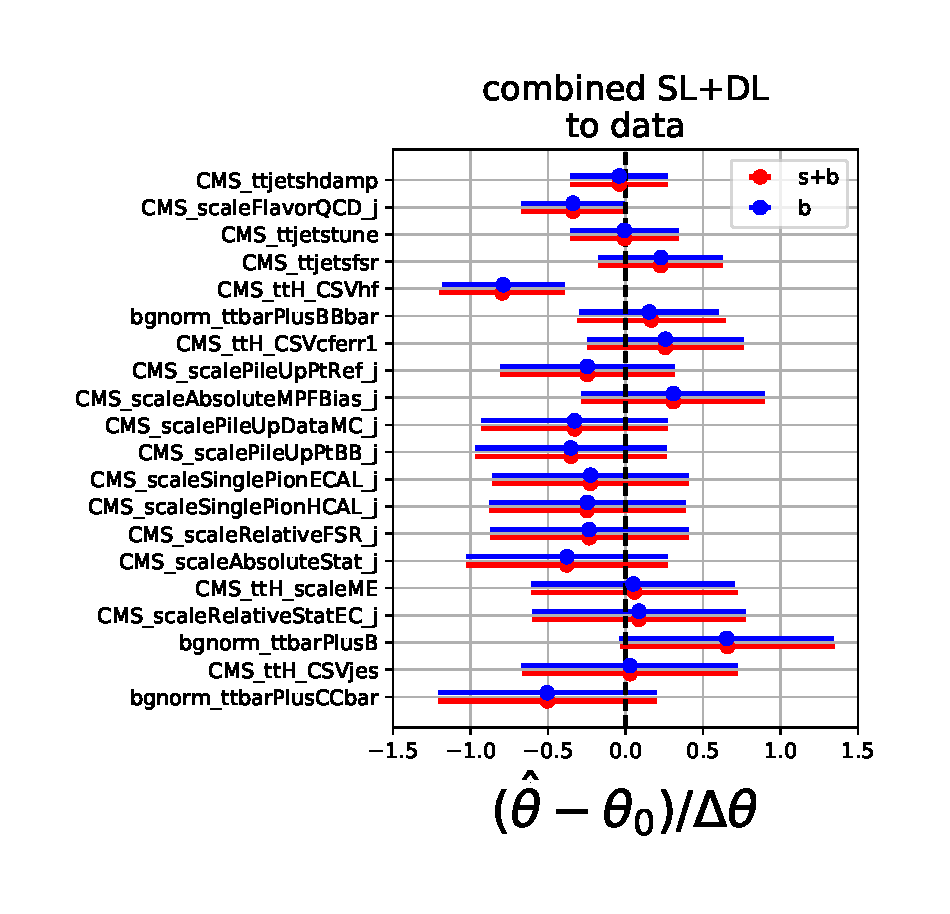
\includegraphics[width=0.5\textwidth]{figures/tth/pulls_group_sldl_r0_20.pdf}}
\subfloat{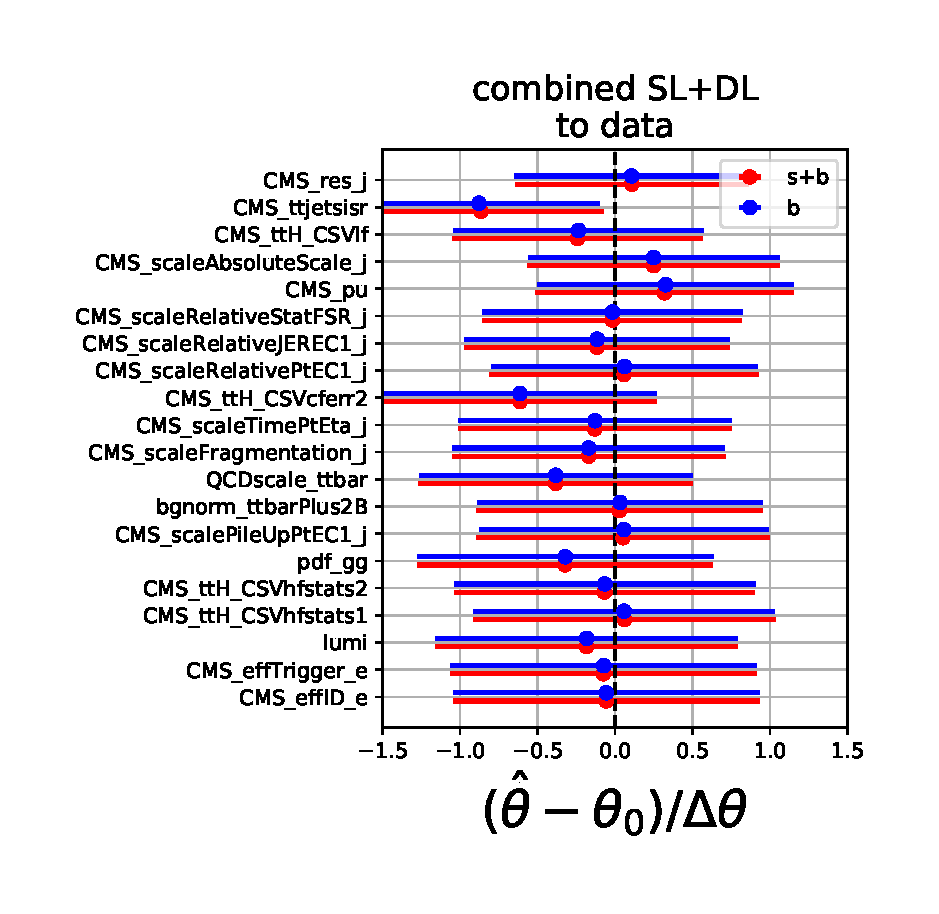
\includegraphics[width=0.5\textwidth]{figures/tth/pulls_group_sldl_r20_40.pdf}}\\
\subfloat{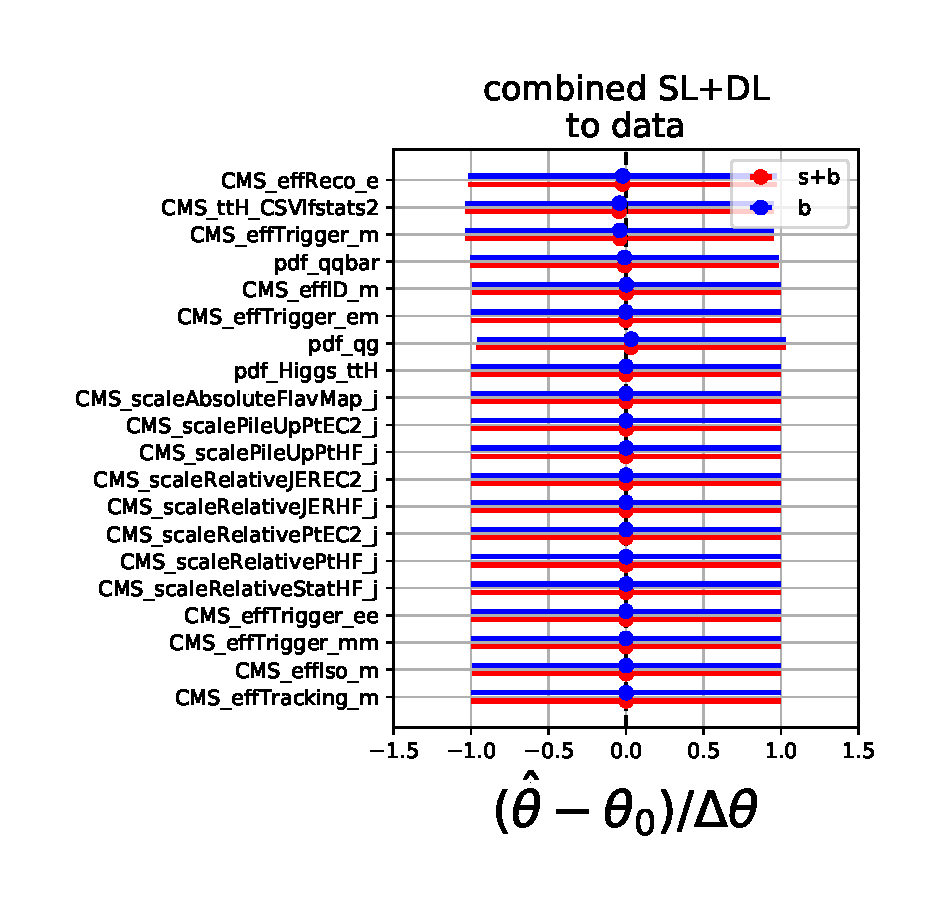
\includegraphics[width=0.5\textwidth]{figures/tth/pulls_group_sldl_r40_60.pdf}}
\caption[The post-fit pulls]{The constraints and pulls on the nuisance parameters, fitting the model to data. We see the strongest constraints for the \ttbar+jets modelling, the JES flavour modelling and the CSV b discriminator heavy flavour modelling.}
\label{fig:tth_sldl_pulls_postfit}
\end{centering}
\end{figure}

We compare the post-fit distributions of the nuisance parameters in~\cref{fig:tth_sldl_pulls_postfit} to the expected distributions in~\cref{fig:tth_sldl_pulls}. In general, we see that the data admit strongest constraints, at the level of $\mathrm{Var}[(\hat{\theta} - \theta_0)/\Delta \theta] \simeq 25\%$ for the nuisance parameters of the \ttbar+jets parton shower modelling. The most significant pull is for the CSV heavy flavour modelling nuisance parameter, at $\langle (\hat{\theta} - \theta_0)/\Delta \theta \rangle \simeq -0.8$. This can be understood as the model compensating for the shape mismodelling of the b~tagging likelihood discriminator.

In order to test the compatibility of the results between the semileptonic and dileptonic categories, we carry out additional fits in the semileptonic and dileptonic categories separately. In the semileptonic channel, we find $\mu = 0.71\pm 0.88$, whereas in the dileptonic channel, the best-fit value for the signal strength parameter is $\mu = -1.61^{+1.25}_{-1.20}$. This is understood to be the effect of the downward fluctuation in data in the dileptonic discriminator distribution. We also find the upper limit on the signal strength at a 95\% confidence level in the combined case and for the SL and DL categories. The results of these fits are shown in~\cref{fig:tth_combined}. Furthermore, the post-fit agreement between the model and the data can be visualised by sorting all the bins of the fitted templates according to the expected signal over background ratio, as shown in~\cref{fig:tth_sob}. Overall, we find the best fit value and the upper limit for the signal strength parameter to be

\begin{align}
\label{eq:tth_bestfit}
\hat{\mu} &= -0.07  ^{+0.27}_{-0.28}~\mathrm{stat} ^{+0.74}_{-0.73}~\mathrm{syst} \\
&= -0.07^{+0.79}_{-0.78}\\
\mu^{95\%CL} &= 1.52~\mathrm{obs.}~(1.57~\mathrm{exp.}).
\end{align}

\begin{figure}
\begin{centering}
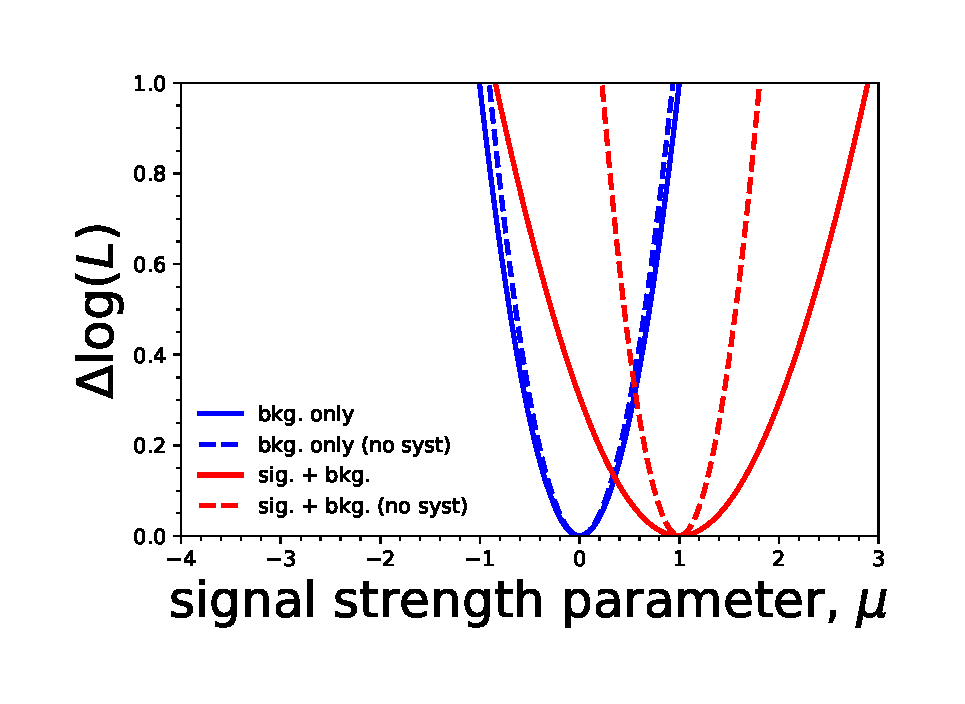
\includegraphics[width = 0.5\textwidth]{figures/tth/r_scan.pdf}
\caption[The likelihood with respect to the minimum as a function of $\mu$]{The likelihood as a function of $\mu$ on the background only ($\mu=0$) Asimov dataset (blue) and the signal+background ($\mu=1$) Asimov dataset. We also see that the uncertainty in $\mu$ is reduced when removing the systematic uncertainties from the model.}
\label{fig:tth_likelihood}
\end{centering}
\end{figure}

The compatibility of the data with the SM hypothesis is at the level of $Z=1.4\sigma$, as shown in~\cref{fig:tth_likelihood}. The data are also compatible with the background only hypothesis. In order to study the compatibility of the combined fit with the individual categories and to understand the contributions of the various categories, we have carried out individual fits in all the categories separately, eight in total. The results are shown in~\cref{fig:tth_limits_category} and in~\cref{tab:limits_category}. In general, we see that the fit in the semileptonic categories prefers a positive signal strength, whereas in the dileptonic categories, a negative signal strength is preferred. This is consistent with the pre-fit distributions and the observed downward fluctuation in the dilepton channel. For these individual fits, the nuisance parameters obtain different and possibly inconsistent values for each fit. Therefore, we have also carried out a multidimensional fit with an individual $\mu$ for each category, but the same nuisance parameters across the categories. The results from this multidimensional fit are compatible with the combined fit with a p-value of $p\simeq0.56$, estimated using toy experiments drawn from MC distributions.

\begin{figure}
\begin{centering}
\subfloat{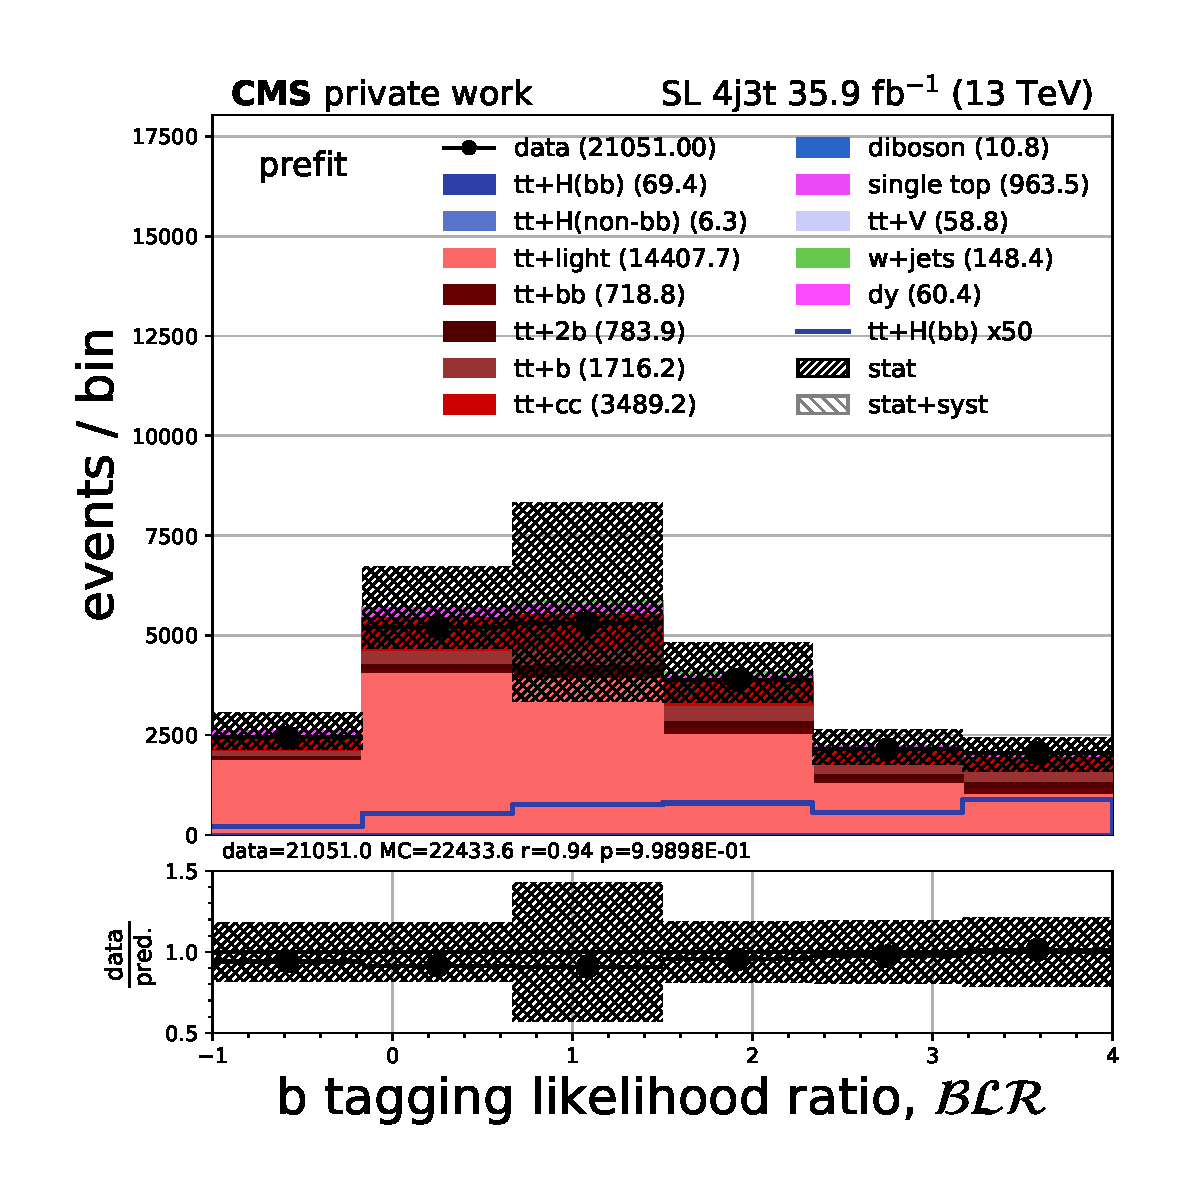
\includegraphics[width=0.5\textwidth]{figures/tth/sl_j4_t3_prefit.pdf}}
\subfloat{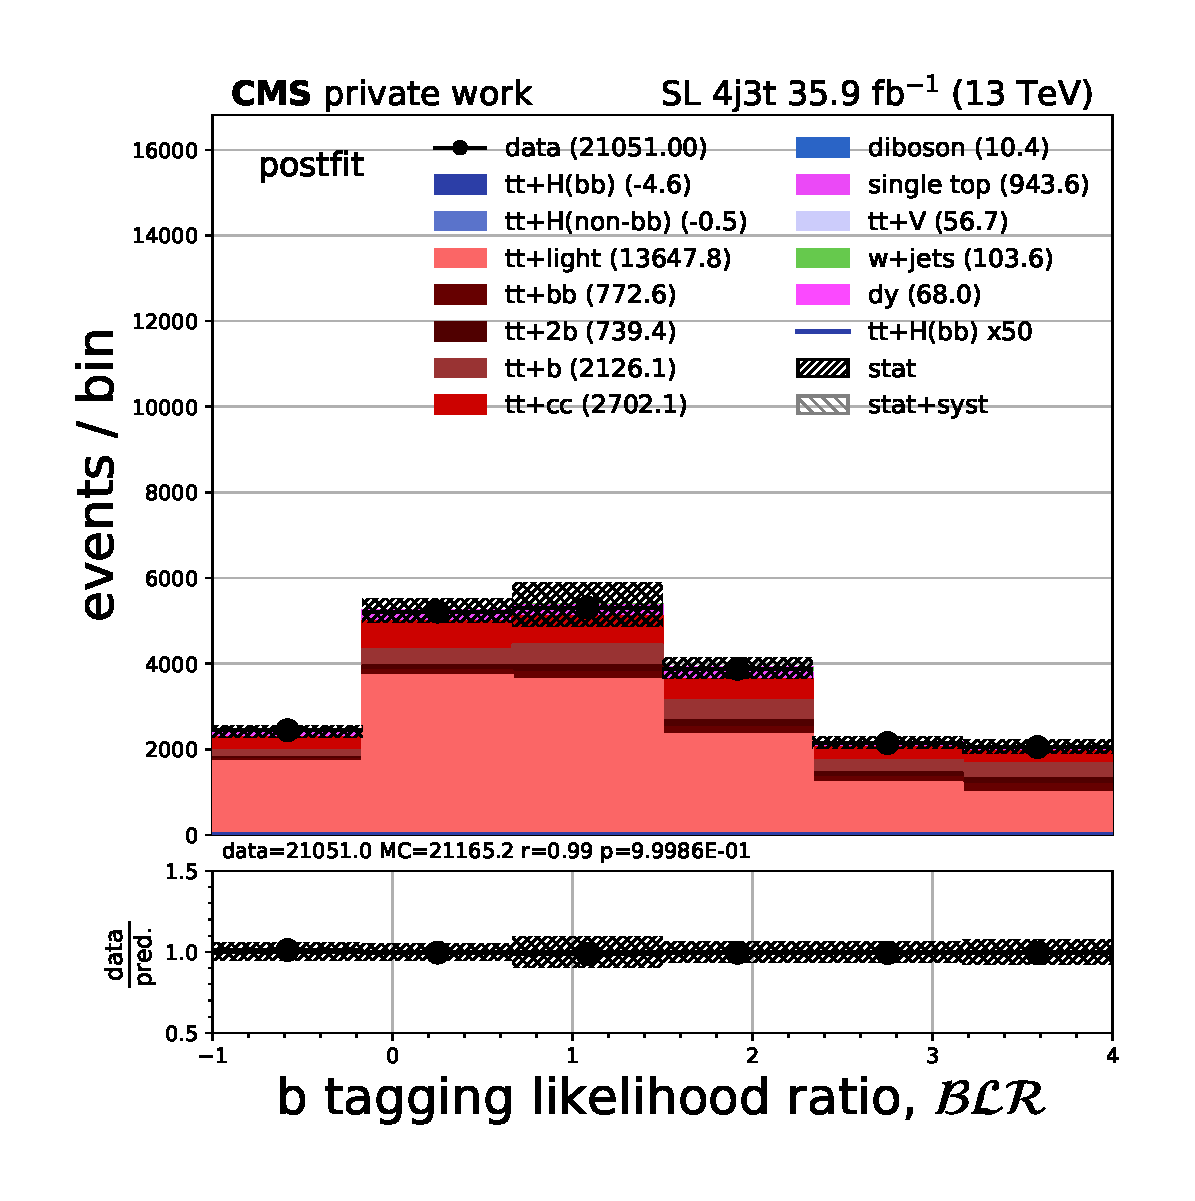
\includegraphics[width=0.5\textwidth]{figures/tth/sl_j4_t3_postfit.pdf}} \\

\subfloat{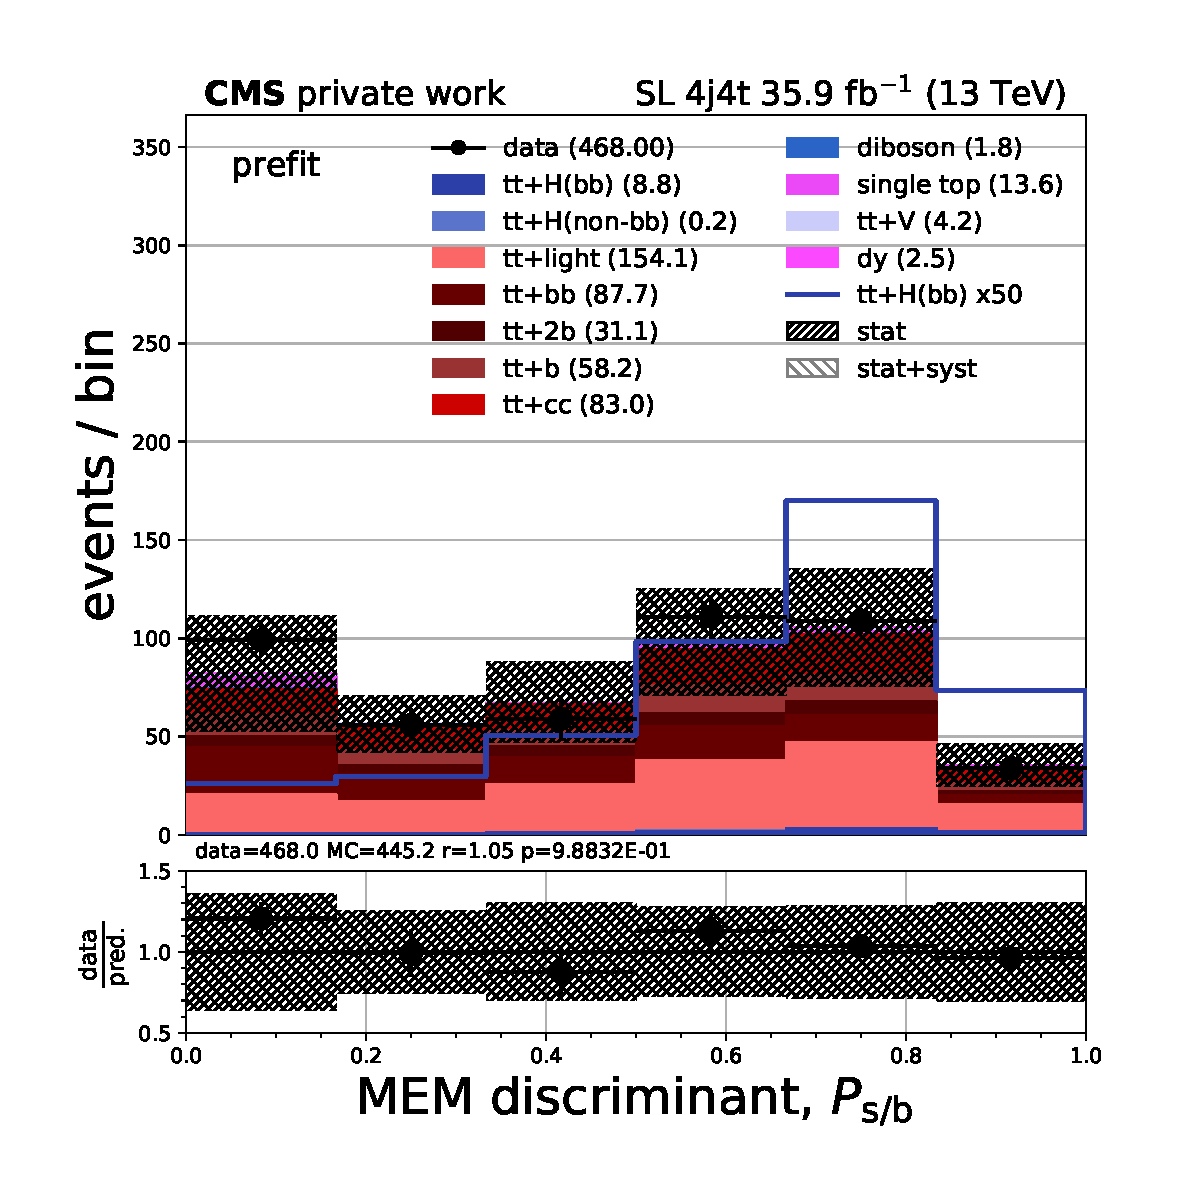
\includegraphics[width=0.5\textwidth]{figures/tth/sl_j4_tge4_prefit.pdf}}
\subfloat{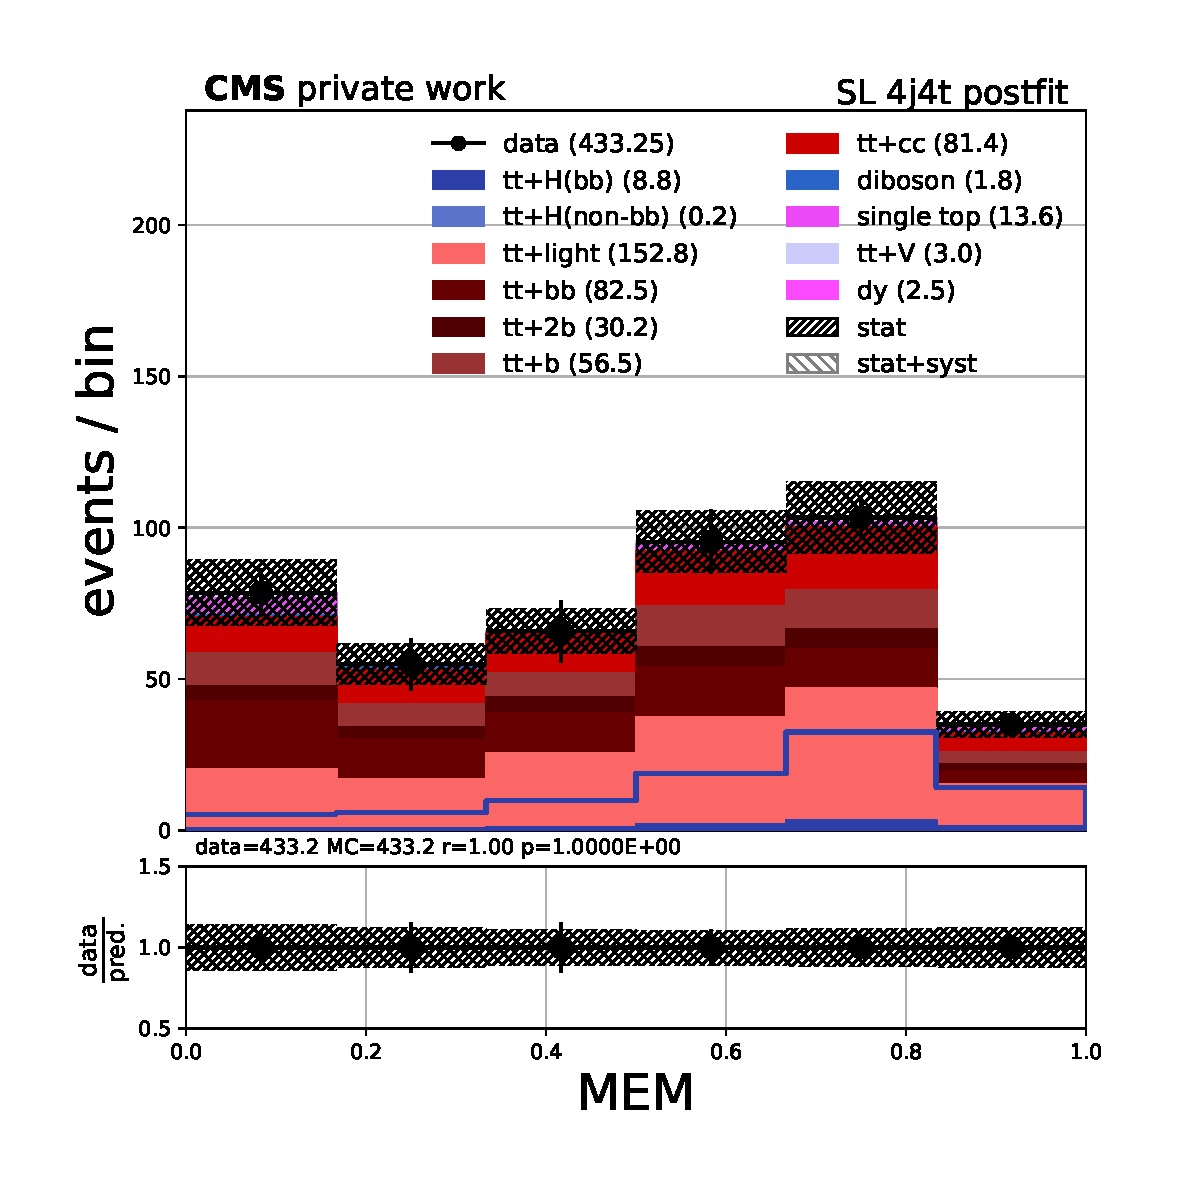
\includegraphics[width=0.5\textwidth]{figures/tth/sl_j4_tge4_postfit.pdf}} \\
\caption[The pre-fit and post-fit distributions in the semileptonic 4-jet categories]{The pre-fit (left column) and post-fit (right column) distributions in the semileptonic 4~jet, 3~b~tag category (top row) and the 4~jet, 4~b~tag category (bottom row).}
\label{fig:tth_postfit1}
\end{centering}
\end{figure}

\begin{figure}
\begin{centering}

\subfloat{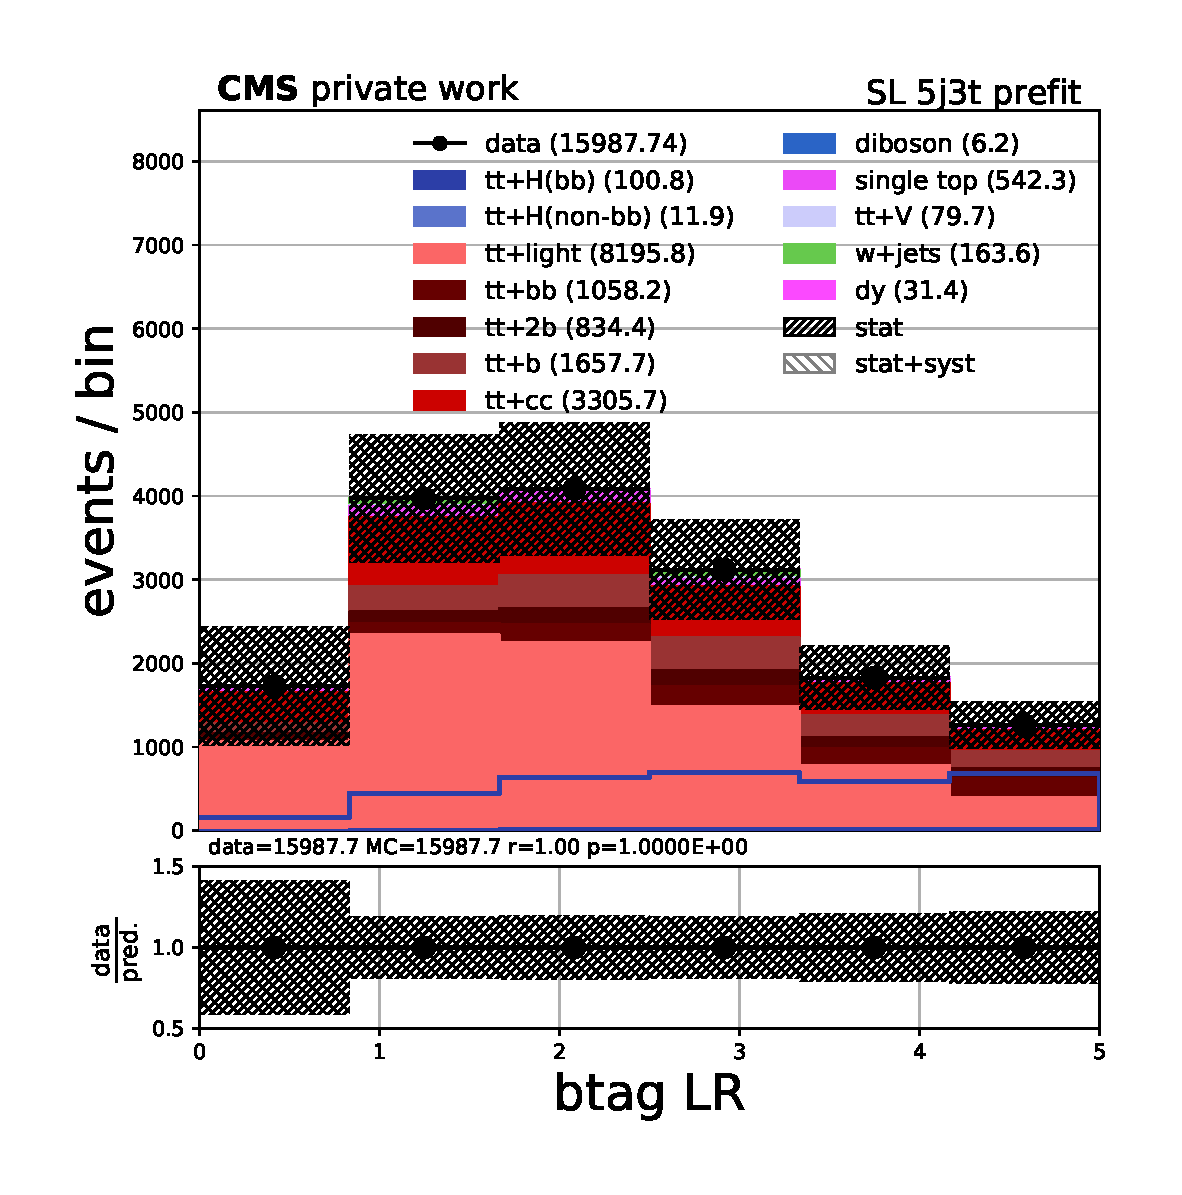
\includegraphics[width=0.5\textwidth]{figures/tth/sl_j5_t3_prefit.pdf}}
\subfloat{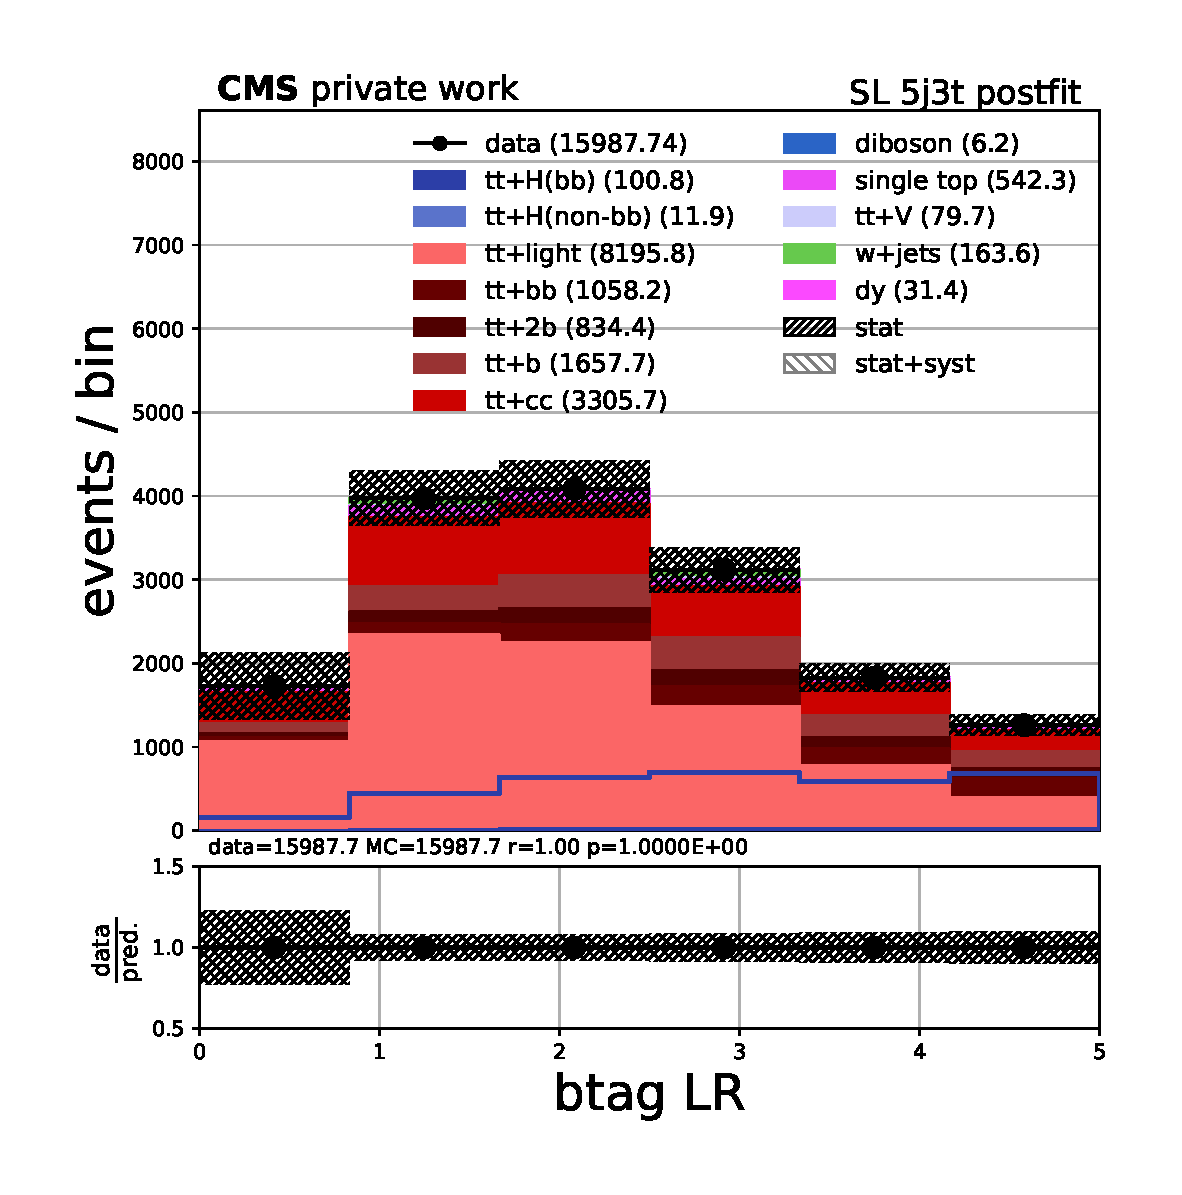
\includegraphics[width=0.5\textwidth]{figures/tth/sl_j5_t3_postfit.pdf}}\\

\subfloat{\includegraphics[width=0.5\textwidth]{figures/tth/sl_j5_tge4_prefit.pdf}}
\subfloat{\includegraphics[width=0.5\textwidth]{figures/tth/sl_j5_tge4_postfit.pdf}}\\

\caption[The pre-fit and post-fit distributions in the semileptonic 5-jet categories]{The pre-fit (left column) and post-fit (right column) distributions in the semileptonic 5~jet 3~b~tag category (top row) and the 5~jet, $\geq4$~b~tag category (bottom row).}
\label{fig:tth_postfit2}
\end{centering}
\end{figure}

\begin{figure}
\begin{centering}
\subfloat{\includegraphics[width=0.5\textwidth]{figures/tth/sl_jge6_t3_prefit.pdf}}
\subfloat{\includegraphics[width=0.5\textwidth]{figures/tth/sl_jge6_t3_postfit.pdf}} \\

\subfloat{\includegraphics[width=0.5\textwidth]{figures/tth/sl_jge6_tge4_prefit.pdf}}
\subfloat{\includegraphics[width=0.5\textwidth]{figures/tth/sl_jge6_tge4_postfit.pdf}} \\
\caption[The pre-fit and post-fit distributions in the semileptonic $\geq6$-jet categories]{The pre-fit (left column) and post-fit (right column) distributions in the semileptonic $\geq6$ jet, 3~b~tag category (top row) and the $\geq6$ jet, $\geq4$~b~tag category (bottom row).}
\label{fig:tth_postfit3}
\end{centering}
\end{figure}

\begin{figure}
\begin{centering}
\subfloat{\includegraphics[width=0.5\textwidth]{figures/tth/dl_jge4_t3_prefit.pdf}}
\subfloat{\includegraphics[width=0.5\textwidth]{figures/tth/dl_jge4_t3_postfit.pdf}}\\

\subfloat{\includegraphics[width=0.5\textwidth]{figures/tth/dl_jge4_tge4_prefit.pdf}}
\subfloat{\includegraphics[width=0.5\textwidth]{figures/tth/dl_jge4_tge4_postfit.pdf}}\\
\caption[The pre-fit and post-fit distributions in the dileptonic categories]{The pre-fit (left column) and post-fit (right column) discriminator distributions in the dileptonic categories, with the $\geq4$~jet, 3~b~tag category in the top row and the $\geq4$~jet, $\geq4$~b~tag category in the bottom row.}
\label{fig:tth_postfit4}
\end{centering}
\end{figure}

\begin{figure}
\begin{centering}
\includegraphics[width = 1.0\textwidth]{figures/tth/nuis_corr.pdf}
\caption[The post-fit correlation between the signal strength parameter and the nuisance parameters]{The post-fit correlation coefficient between the signal strength parameter $\mu$ and the nuisance parameters. We see an anti-correlation at the level of 30\% between the signal strength modifier and the \ttbb\xspace normalisation. Furthermore, we find that there is non-negligible residual correlation between the uncertainties.}
\label{fig:tth_corr}
\end{centering}
\end{figure}

\begin{figure}
\begin{centering}
\subfloat{\includegraphics[width = 0.6\textwidth]{figures/tth/bestfit.pdf}} 
\subfloat{\includegraphics[width = 0.5\textwidth]{figures/tth/limits_comb.pdf}} 
\caption[The best-fit value and the 95\% upper limits on the signal strength parameter]{The best-fit values (left) and the 95\% upper limits (right) on the signal strength parameter in the semileptonic and dileptonic categories and the combined fit.}
\label{fig:tth_combined}
\end{centering}
\end{figure}

\begin{figure}
\begin{centering}
\includegraphics[width = 0.8\textwidth]{figures/tth/sob.pdf}
\caption[The final analysis bins, arranged by the signal over background ratio $S/B$]{The best-fit signal and background distributions in the bins of the final discriminant, arranged by $S/B$, along with the measured data. In determining the uncertainty of the background prediction, we have neglected correlations between the uncertainties of the bins. We show the expected SM \ttH~process in red and the measured value, scaled up by a factor of 10, in blue.}
\label{fig:tth_sob}
\end{centering}
\end{figure}

\begin{figure}
\begin{centering}
\includegraphics[width = 0.8\textwidth]{figures/tth/limits.pdf}
\caption[The expected and observed upper limits on the signal strength parameter.]{The expected and observed upper limits on the signal strength parameter at a 95\% confidence limit in the analysis categories. We show the 95\% and 68\% range of expected limit under no signal, along with the median of the distribution. This can be compared to the expected limit when a nominal SM signal is injected. We also show the observed limit. The numerical values can be found in~\cref{tab:limits_category}.}
\label{fig:tth_limits_category}
\end{centering}
\end{figure}


\begin{table}
\def\arraystretch{1.5}
\begin{center}
\begin{tabular}{l|c|cccc}
\hline
\multirow{2}{*}{category} & \multirow{2}{*}{best fit $\mu$} & \multicolumn{3}{c}{95\% upper limit on $\mu$}\\
 & & expected & observed & injected \\
\hline
DL $\geq$4j 3t & $-1.93^{+5.87}_{-7.24}$ & $10.91^{15.21}_{7.90}$ & $9.91$ & $12.28$ \\
DL $\geq$4j $\geq$4t & $-1.51^{+1.26}_{-1.23}$ & $3.01^{4.53}_{2.06}$ & $2.03$ & $3.97$ \\
\hline
DL & $-1.61^{+1.25}_{-1.20}$ & $3.04^{4.55}_{2.09}$ & $1.96$ & $3.94$ \\
\hline
SL 4j3t & $9.21^{+10.79}_{-15.86}$ & $31.12^{43.41}_{22.57}$ & $39.04$ & $28.52$ \\
SL 4j4t & $0.34^{+6.05}_{-5.89}$ & $12.09^{17.35}_{8.56}$ & $12.43$ & $12.51$ \\
SL 5j3t & $7.94^{+8.32}_{-9.83}$ & $17.81^{24.84}_{12.90}$ & $22.79$ & $16.14$ \\
SL 5j $\geq$ 4t & $1.73^{+2.56}_{-2.47}$ & $5.11^{7.41}_{3.59}$ & $6.53$ & $5.64$ \\
SL $\geq$6j $3$t & $0.53^{+5.78}_{-7.32}$ & $11.00^{15.12}_{8.12}$ & $11.32$ & $11.07$ \\
SL $\geq$6j $\geq$4t & $1.25^{+1.34}_{-1.36}$ & $2.63^{3.80}_{1.85}$ & $3.66$ & $3.46$ \\
\hline
SL & $0.71^{+0.88}_{-0.88}$ & $1.80^{2.57}_{1.29}$ & $2.33$ & $2.61$ \\
\hline
comb. & $-0.07^{+0.78}_{-0.79}$ & $1.57^{2.24}_{1.11}$ & $1.52$ & $2.37$ \\
\hline
\hline
\end{tabular}
\caption[The best-fit values and upper limits per category]{The best-fit values on the signal strength parameter $\mu$, along with the median expected limit, the 68\% confidence interval on the limit and the observed upper limits on $\mu$ at a 95\% CL. For comparison, we also list the expected limit when injecting a signal with $\mu=1$.}
\label{tab:limits_category}
\end{center}
\end{table}

\subsection{Systematic uncertainties}
After fitting the model to data, we determine the impacts of the major uncertainties on the signal strength parameter, with the results shown in~\cref{tab:systematic_uncertainties_posterior}. These are found by freezing a particular set of nuisance parameters and determining the change in the post-fit uncertainty on $\mu$, under the assumption that the uncertainties are uncorrelated. This assumption holds only approximately, as can be seen from the correlation matrix in~\cref{fig:tth_corr}, thus the individual uncertainty components cannot be treated as independent and Gaussian-distributed, i.e. they cannot be added in quadrature.

Overall, we see from~\cref{tab:systematic_uncertainties_posterior} that this analysis is dominated by systematic uncertainties ($\Delta \mu \simeq \pm 0.73$) in the theoretical modelling ($\Delta \mu \simeq \pm 0.53$)  of the background processes ($\Delta \mu \simeq \pm 0.32$). The considerable normalisation uncertainties assigned to the various \ttbar+heavy flavour processes, specifically the \ttbb~process, have a significant effect on the analysis. The second largest source of theoretical uncertainty is the parton shower modelling of the initial state radiation with $\Delta \mu \simeq \pm 0.15$, which affects the predicted yield of the \ttbar+jets background. This is followed by uncertainties on the ME scale with $\Delta \mu \simeq \pm 0.13$, resulting in distortions to the final discriminant shapes.

We have studied the sources of uncertainty in more detail by evaluating the shift in the best-fit value of the signal strength parameter when the nuisance parameters are shifted around their post-fit values by one standard deviation. These results are shown in~\cref{fig:tth_impacts}, where we see that the \ttbb~normalisation uncertainty and the modelling of the ISR have the largest impacts on the signal strength.

Out of the experimental factors, the major sources of uncertainty are MC simulation statistics with $\Delta \mu \simeq \pm 0.25$, which remains a challenge in the high-multiplicity final state, followed by the detailed modelling of the experimental observables related to b~tagging with $\Delta \mu \simeq \pm 0.23$ and jet energy corrections with $\Delta \mu \simeq \pm 0.11$. In general, all these sources of uncertainty have considerable effects on the predicted number of events and the distributions of the final discriminators in the analysis categories, such that the final nuisance parameters have non-negligible correlations, for example the nuisance parameters for the CSV heavy flavour and charm flavour modelling are anti-correlated with $\rho \simeq -0.4$, as seen in~\cref{fig:tth_corr}.

\begin{figure}
\begin{centering}
\includegraphics[width = 0.8\textwidth]{figures/tth/impacts.pdf}
\caption[The impact of nuisance parameters on the signal strength.]{The impact of nuisance parameters on the signal strength. The impacts are derived by shifting the nuisance parameter under question by one standard deviation up or down around the post-fit value $\hat{\theta}$ and computing the change in the best-fit signal strength value. We see the most significant impacts from the \ttbb~uncertainty, followed by the heavy flavour b~tagging uncertainty and the parton shower modelling uncertainties. The impact of some nuisance parameters, such as the JES modelling in the CSV b discriminator, may be one-sided, i.e. always positive or negative. This happens when the other nuisance parameters are able to compensate for the shift in this particular nuisance parameter. In comparison to the data in~\cref{tab:systematic_uncertainties_posterior}, we list the impacts of individual nuisance parameters, instead of logical groups of nuisances. We omit the uncertainties from the limited MC statistics from this list.}
\label{fig:tth_impacts}
\end{centering}
\end{figure}

\begin{table}
\begin{center}
\begin{tabular}{c|cc}
uncertainty source & $-\Delta\mu$ & $+\Delta\mu$ \\
\hline
bkg. norm. & $-0.32$ & $+0.25$\\
ISR, FSR & $-0.13$ & $+0.15$\\
pdf norm. & $-0.00$ & $+0.04$\\
$Q^2$ scale & $-0.13$ & $+0.11$\\
MC tune, $h_{\mathrm{damp}}$ & $-0.03$ & $+0.05$\\
\hline
theory & $-0.53$ & $+0.49$\\
\hline
MC stats & $-0.25$ & $+0.24$\\
JES, JER & $-0.11$ & $+0.09$\\
b~tagging & $-0.23$ & $+0.16$\\
PU, lumi, lepton & $-0.08$ & $+0.08$\\
\hline
experimental & $-0.35$ & $+0.30$\\
\hline
systematic & $-0.72$ & $+0.71$\\
statistical & $-0.31$ & $+0.31$\\
total & $-0.79$ & $+0.78$\\
\hline
\hline
\end{tabular}
\caption[The post-fit uncertainties in the~\ttHbb\xspace analysis]{The post-fit uncertainties on the signal strength parameter $\mu$ in the~\ttHbb\xspace analysis. The uncertainties are estimated by freezing sets of nuisance parameters in the fit and evaluating the change in post-fit uncertainty with respect to the nominal case. Due to correlations, the uncertainties of the experimental and theory groups cannot be added in quadrature.}
\label{tab:systematic_uncertainties_posterior}
\end{center}
\end{table}

\section{Discussion}
\label{sec:tth_discussion}
This result has been derived using the 2016 dataset from CMS at $\sqrt{s} = 13$~TeV corresponding to an integrated luminosity of $35.9~\ifb$. We can compare it to the equivalent CMS analysis at $\sqrt{s} = 8$~TeV~\cite{Khachatryan:2015ila} with $19.5~\ifb$ of data, where a similar analysis strategy with the MEM was employed, and to the latest result on \ttHbb~from the ATLAS collaboration~\cite{ATLAS:2017nkr} with $36.1~\ifb$ of data.

We see from the comparison in~\cref{tab:tth_results_comparison} that this work improves by about a factor of 2 in sensitivity over the equivalent search of CMS at 8 TeV. This can be attributed partly to the increased dataset, but also to the favourable centre-of-mass scaling of the cross-section ratio for signal $\sigma_{\ttH}^{13~\mathrm{TeV}}/\sigma_{\ttH}^{8~\mathrm{TeV}} \simeq 3.9$ and background $\sigma_{\ttbar+\mathrm{jets}}^{13~\mathrm{TeV}}/\sigma_{\ttbar+\mathrm{jets}}^{8~\mathrm{TeV}} \simeq 3.3$ and the improved reconstruction and background rejection, with the signal-over-background fraction improving from $3.4\%$ in the highest purity category at 8 TeV to $4.2\%$ at 13 TeV. The main sources of systematic uncertainties affecting this analysis have not changed with respect to the 8 TeV analysis. In particular, the dominant source of uncertainty in both cases is the 50\% normalisation uncertainty on the \ttbb~background. Although recent analyses from CMS have determined the \ttbb~cross-section to a relative precision of about $\simeq30\%$, it is compatible with the post-fit constraints that we observe in this work and thus a more precise measurement would be needed to significantly reduce the effect of this uncertainty. Furthermore, in the aforementioned analysis, the \ttHbb~process is considered as a background for the \ttbb~measurement, thus, any \ttHbb~signal would be absorbed into the \ttbb~normalisation. A possible direction of future research would be the consistent and simultaneous measurement of \ttHbb~and \ttbb~in a multidimensional fit.

It is interesting to compare the work presented in this thesis to the latest results from ATLAS, where an equivalent dataset is used. First, we see that the sensitivity of the ATLAS analysis is about $\simeq20\%$ higher than that reported in this work. This is likely due to the significantly more complex statistical analysis techniques employed in the ATLAS analysis, in particular a staged approach with a BDT that is responsible for choosing the optimal reconstruction hypothesis for the observed jets, followed by another classification BDT optimised to distinguish between signal and background. These algorithms are optimised on simulation on an event-by-event basis and rely heavily on the detailed modelling of b~tagging discriminators. For comparison, only the MEM and the b~tagging likelihood ratio classifiers are used in this work, neither of which require significant MC simulation to be evaluated on a new dataset. Furthermore, ATLAS is already making use of improved vertexing and b-tagging in the detector through the Insertable B-Layer~\cite{Capeans:1291633}. A similarly-upgraded pixel detector is available at CMS since the beginning of 2017~\cite{CMS:2012sda}.

In terms of uncertainties, the ATLAS analysis has a slightly different treatment of the \ttbar+jets modelling and the corresponding uncertainty, where the subcomponents of the default \powheg~MC sample are scaled to an NLO \ttbb~sample generated using \sherpa+\openloops~in the 4-flavour scheme. This scaling is most significant for events with more than one jet containing multiple b hadrons, which make up between 1-2\% of the full \ttbb~cross-section~\cite{ATLAS:2017nkr}. In our analysis, all events with at least one jet containing multiple b hadrons are grouped under the \tttwob~process. In the ATLAS analysis, the systematic uncertainties on the NLO modelling are derived by comparing the nominal \powheg~model to a 5-flavour \sherpa+\openloops~model and independently a 4-flavour model. The normalisation of the various \ttbar+jets subprocesses is left freely floating in the fit, described by $k$-factors. Overall, the CMS and ATLAS procedures for the \ttbar+jets modelling uncertainties are different, but in both cases, the background modelling uncertainties have the largest impacts. The ATLAS analysis observes a post-fit scale factor of $k(\ttbar+\geq\mathrm{1b}) = 1.24 \pm 0.1$ for the \ttbb~process, whereas in the analysis presented in this thesis, the post-fit $k$-factor for this process is consistent with unity. The parton shower modelling uncertainties are estimated by comparing \herwig~and \pythia, whereas for this analysis, it is obtained by varying the parameters in the nominal \powheg+\pythia~model, as explained in~\cref{sec:theory_unc}. Both the ATLAS analysis and the analysis presented in this thesis are mainly impacted by similar systematic uncertainties: the \ttbar+jets modelling, limited MC statistics, b-tagging and JES. It is also clear that it is necessary for the experiments to adopt an improved theoretical model of the \ttbb~process in a way that is consistent and comparable between the experiments.

During 2017, the CMS experiment has recorded approximately $45~\ifb$ of proton-proton collision data at $\sqrt{s}=13~\mathrm{TeV}$. Furthermore, the upgrade of the pixel detector and the commissioning of improved b~tagging algorithms promises to improve the sensitivity of this analysis. On the other hand, progress will need to be made in incorporating the latest improvements in the theoretical modelling, in particular, the NLO 4-flavour models for \ttbb~properly matched to an accurate parton shower.

\begin{table}
\def\arraystretch{1.5}
\begin{center}
\begin{tabular}{cc|ccc}
category & quantity & CMS (8 TeV) & ATLAS (13 TeV) & this work \\
\hline
\multirow{3}{*}{SL} & best-fit $\mu$ & $1.7^{+2.0}_{-1.8}$ & $0.95^{+0.65}_{-0.62}$ & $0.71^{+0.88}_{-0.88}$ \\
 & exp. UL & $4.2^{6.2}_{2.9}$ & $1.4^{1.99}_{1.01}$ & $1.80^{2.57}_{1.29}$ \\
 & obs. UL & $5.5$ & $1.95$ & $2.33$ \\
 \hline
 \multirow{3}{*}{DL} & best-fit $\mu$ & $1.0^{+3.3}_{-3.0}$ & $-0.24^{+1.02}_{-1.05}$ & $-1.61^{+1.25}_{-1.20}$ \\
 & exp. UL & $6.9^{15.8}_{3.4}$ & $2.74^{3.86}_{1.98}$ & $3.04^{4.55}_{2.09}$ \\
 & obs. UL & $7.7$ & $2.64$ & $1.96$ \\
 \hline
 \multirow{3}{*}{combined} & best-fit $\mu$ & $1.2^{+1.6}_{-1.5}$ & $0.84^{+0.64}_{-0.61}$ & $-0.07^{+0.78}_{-0.79} $ \\
 & exp. UL & $3.3^{4.9}_{2.3}$ & $1.24^{1.77}_{0.89}$ & $1.57^{2.24}_{1.11}$ \\
 & obs. UL & $4.2$ & $1.96$ & $1.52$ \\
\end{tabular}
\caption[Comparison of the CMS and ATLAS results on \ttHbb]{A comparison of the CMS~\cite{Khachatryan:2015ila} and ATLAS~\cite{ATLAS:2017nkr} results on \ttHbb~and the results obtained in this work. We compare the best-fit $\mu$, the expected 95\% upper limit (UL) under the no signal hypothesis with $\pm1\sigma$ uncertainties and the observed upper limit.}
\label{tab:tth_results_comparison}
\end{center}
\end{table}

\section{Summary}
\label{sec:tth_summary}
We have presented a search for the \ttH\xspace process in the data collected by the CMS experiment during the 2016 run period, in the channels where the Higgs boson decays to b~quarks and at least one of the top quarks decays leptonically. The observation of this process, where the Higgs boson is produced in association with top quarks, would make it possible to directly study the process of mass generation for up-type quarks and to confirm the mechanism of electroweak symmetry breaking for the heaviest known quark. The analysis is challenging due to the presence of a significant background arising from the QCD production of \ttbar+jets. Specifically, the \ttbb\xspace process, where two additional b~quarks are produced in the final state in association with the top quark pair, is irreducible with respect to the particles in the final state, as we expect between four to six jets, out of which four arise from b~quarks from both the \ttbb~background and the \ttHbb\xspace signal. Furthermore, the analysis is complicated by the presence of a combinatorial self-background, as we cannot directly reconstruct the Higgs boson candidate invariant mass peak due to the presence of several additional b~quark candidates arising from the top decay.

We have shown that it is possible to construct a discriminator based on the direct computation of matrix elements from the kinematic properties of the observed jets and leptons in the event, without relying on large amounts of MC simulation for the \ttbb\xspace process, which is affected by considerable theoretical uncertainties. The observed data are compatible with both the SM signal hypothesis and the background-only hypothesis. We have been able to establish an upper limit on the signal strength modifier at the level of $\mu < 1.52$ at a confidence level of 95\%, with $\mu < 1.57$ expected under the SM hypothesis. The best fit signal strength value is $\mu = -0.07  ^{+0.28}_{-0.27}~\mathrm{(stat.)} ^{+0.73}_{-0.74}~\mathrm{(syst.)}$, with the total combined uncertainty being $\Delta\mu \simeq \pm 0.79$. The largest components in the final uncertainty are of systematic origin, arising from the modelling of the \ttbar+heavy flavour background and the overall theoretical uncertainties in the modelling of the \ttbar+jets background.

Additionally, we find simulation statistics and experimental uncertainties in the detailed calibration of the b~discriminator shape to have a sub-leading but significant effect on the final measurement. This means that in addition to an improved theoretical treatment of the \ttbar+jets background, which is crucial for this analysis, improving the MC simulation in terms of a more efficient use of the generated events and an improved modelling of the quantities related to b~tagging can improve this analysis. Both of these problems are well-suited to be solved with the matrix element method discriminator, which does not rely on the precise modelling of various low-level experimental observables such as b~discriminator distributions or extensive simulation statistics.

It is expected that the dataset from the 2017 run period will allow us to further improve our understanding of the \ttH~process, where the \Hbb~decay channel benefits from a high branching ratio. The discovery of the \ttH~production mode at a $5\sigma$ significance level is feasible within 2018 through a combination of multiple channels and datasets. However, a focused experimental and theoretical effort is needed to fully make use of these additional data, as this analysis is affected by significant systematic uncertainties.
